\documentclass[12pt,chapterheads,oneside]{ucsd}

\usepackage{amsmath, amscd, amssymb, amsthm}
\usepackage{graphicx}
\usepackage{xfrac}
\usepackage{color}
\usepackage{multirow}
\usepackage{multicol}
\usepackage{ifthen}
\usepackage{xspace}
\usepackage{calc}
%\usepackage{slashbox}
\usepackage{subfig}
\usepackage[T1]{fontenc}
\usepackage{mathptmx}
\usepackage{makeidx}
\usepackage[bottom]{footmisc}
\usepackage[hyphens]{url}
\usepackage[color=red!40,textwidth=24mm,textsize=footnotesize]{todonotes}
\usepackage[hidelinks,linktocpage,breaklinks]{hyperref}                                  
\usepackage{rotating}
\usepackage{afterpage}
\usepackage{xparse}
\usepackage{lineno}
\usepackage{slashed}
\usepackage{bm}

\hypersetup{ pdfauthor   = {Ian MacNeill},
             pdftitle    = {Measurement of top quark-antiquark pair production in association with a Z boson with a trilepton final state in pp collisions at \sqrt{s} = 8 TeV},
             pdfkeywords = {LHC CERN CMS top Standard Model SM Ian MacNeill},
             pdfcreator  = {LaTeX with hyperref package},
             pdfproducer = {LaTeX} }

%%%%%%%%%%%%%%%%%%%%%%%%%%%%%%%%%%%%%%%%%%%%%%%%%%%%%%%%%%%%%%%%%%%%
%
%  CMS Common definitions style file
%
%  N.B. use of \newcommand rather than \newcommand means
%       that a definition is ignored if already specified
%
%                                              L. Taylor 18 Feb 2005
%%%%%%%%%%%%%%%%%%%%%%%%%%%%%%%%%%%%%%%%%%%%%%%%%%%%%%%%%%%%%%%%%%%%

% Some shorthand
% turn off italics
\newcommand {\etal}{\mbox{et al.}\xspace} %et al. - no preceding comma
\newcommand {\ie}{\mbox{i.e.}\xspace}     %i.e.
\newcommand {\eg}{\mbox{e.g.}\xspace}     %e.g.
\newcommand {\etc}{\mbox{etc.}\xspace}     %etc.
\newcommand {\vs}{\mbox{\sl vs.}\xspace}      %vs.
\newcommand {\mdash}{\ensuremath{\mathrm{-}}} % for use within formulas

% some terms whose definition we may change
\newcommand {\Lone}{Level-1\xspace} % Level-1 or L1 ?
\newcommand {\Ltwo}{Level-2\xspace}
\newcommand {\Lthree}{Level-3\xspace}

% Some software programs (alphabetized)
\newcommand{\ACERMC} {\textsc{AcerMC}\xspace}
\newcommand{\ALPGEN} {{\textsc{alpgen}}\xspace}
\newcommand{\CHARYBDIS} {{\textsc{charybdis}}\xspace}
\newcommand{\CMKIN} {\textsc{cmkin}\xspace}
\newcommand{\CMSIM} {{\textsc{cmsim}}\xspace}
\newcommand{\CMSSW} {{\textsc{cmssw}}\xspace}
\newcommand{\COBRA} {{\textsc{cobra}}\xspace}
\newcommand{\COCOA} {{\textsc{cocoa}}\xspace}
\newcommand{\COMPHEP} {\textsc{CompHEP}\xspace}
\newcommand{\CTTEN} {\textsc{cteq10}\xspace}
\newcommand{\EVTGEN} {{\textsc{evtgen}}\xspace}
\newcommand{\FAMOS} {{\textsc{famos}}\xspace}
\newcommand{\GARCON} {\textsc{garcon}\xspace}
\newcommand{\GARFIELD} {{\textsc{garfield}}\xspace}
\newcommand{\GEANE} {{\textsc{geane}}\xspace}
\newcommand{\GEANTfour} {{\textsc{geant4}}\xspace}
\newcommand{\GEANTthree} {{\textsc{geant3}}\xspace}
\newcommand{\GEANT} {{\textsc{geant}}\xspace}
\newcommand{\HDECAY} {\textsc{hdecay}\xspace}
\newcommand{\HERWIG} {{\textsc{herwig}}\xspace}
\newcommand{\HIGLU} {{\textsc{higlu}}\xspace}
\newcommand{\HIJING} {{\textsc{hijing}}\xspace}
\newcommand{\IGUANA} {\textsc{iguana}\xspace}
\newcommand{\ISAJET} {{\textsc{isajet}}\xspace}
\newcommand{\ISAPYTHIA} {{\textsc{isapythia}}\xspace}
\newcommand{\ISASUGRA} {{\textsc{isasugra}}\xspace}
\newcommand{\ISASUSY} {{\textsc{isasusy}}\xspace}
\newcommand{\ISAWIG} {{\textsc{isawig}}\xspace}
\newcommand{\JIMMY} {{\textsc{jimmy}}\xspace}
\newcommand{\MADGRAPH} {\textsc{MadGraph}\xspace}
\newcommand{\MSTW} {\textsc{mstw2008}\xspace}
\newcommand{\NNPDF} {\textsc{nnpdf}\xspace}
\newcommand{\GGTWW}  {{\textsc{gg2ww}}\xspace}
\newcommand{\POWHEG} {\textsc{powheg}\xspace}
\newcommand{\HqT} {\textsc{HqT}\xspace}
\newcommand{\MCATNLO} {\textsc{mc@nlo}\xspace}
\newcommand{\MCFM} {\textsc{mcfm}\xspace}
\newcommand{\FEWZ} {\textsc{fewz}\xspace}
\newcommand{\MILLEPEDE} {{\textsc{millepede}}\xspace}
\newcommand{\ORCA} {{\textsc{orca}}\xspace}
\newcommand{\OSCAR} {{\textsc{oscar}}\xspace}
\newcommand{\PHOTOS} {\textsc{photos}\xspace}
\newcommand{\PROSPINO} {\textsc{prospino}\xspace}
\newcommand{\PYTHIA} {{\textsc{pythia}}\xspace}
\newcommand{\SHERPA} {{\textsc{sherpa}}\xspace}
\newcommand{\TAUOLA} {\textsc{tauola}\xspace}
\newcommand{\TOPREX} {\textsc{TopReX}\xspace}
\newcommand{\XDAQ} {{\textsc{xdaq}}\xspace}


%  Experiments
\newcommand {\DZERO}{D0\xspace}     %etc.


% Measurements and units...

\newcommand{\de}{\ensuremath{^\circ}}
\newcommand{\ten}[1]{\ensuremath{\times \text{10}^\text{#1}}}
\newcommand{\unit}[1]{\ensuremath{\text{\,#1}}\xspace}
\newcommand{\mum}{\ensuremath{\,\mu\text{m}}\xspace}
\newcommand{\micron}{\ensuremath{\,\mu\text{m}}\xspace}
\newcommand{\cm}{\ensuremath{\,\text{cm}}\xspace}
\newcommand{\cmcm}{\ensuremath{\,\text{cm^2}}\xspace}
\newcommand{\s}{\ensuremath{\,\text{s}}\xspace}
\newcommand{\ns}{\ensuremath{\,\text{ns}}\xspace}
% \newcommand{\mm}{\ensuremath{\,\text{mm}}\xspace}
\newcommand{\mus}{\ensuremath{\,\mu\text{s}}\xspace}
\newcommand{\keV}{\ensuremath{\,\text{ke\hspace{-.08em}V}}\xspace}
\newcommand{\MeV}{\ensuremath{\,\text{Me\hspace{-.08em}V}}\xspace}
\newcommand{\GeV}{\ensuremath{\,\text{Ge\hspace{-.08em}V}}\xspace}
\newcommand{\gev}{\GeV}
\newcommand{\TeV}{\ensuremath{\,\text{Te\hspace{-.08em}V}}\xspace}
\newcommand{\PeV}{\ensuremath{\,\text{Pe\hspace{-.08em}V}}\xspace}
\newcommand{\keVc}{\ensuremath{{\,\text{ke\hspace{-.08em}V\hspace{-0.16em}/\hspace{-0.08em}}c}}\xspace}
\newcommand{\MeVc}{\ensuremath{{\,\text{Me\hspace{-.08em}V\hspace{-0.16em}/\hspace{-0.08em}}c}}\xspace}
\newcommand{\GeVc}{\ensuremath{{\,\text{Ge\hspace{-.08em}V\hspace{-0.16em}/\hspace{-0.08em}}c}}\xspace}
\newcommand{\TeVc}{\ensuremath{{\,\text{Te\hspace{-.08em}V\hspace{-0.16em}/\hspace{-0.08em}}c}}\xspace}
\newcommand{\keVcc}{\ensuremath{{\,\text{ke\hspace{-.08em}V\hspace{-0.16em}/\hspace{-0.08em}}c^\text{2}}}\xspace}
\newcommand{\MeVcc}{\ensuremath{{\,\text{Me\hspace{-.08em}V\hspace{-0.16em}/\hspace{-0.08em}}c^\text{2}}}\xspace}
\newcommand{\GeVcc}{\ensuremath{{\,\text{Ge\hspace{-.08em}V\hspace{-0.16em}/\hspace{-0.08em}}c^\text{2}}}\xspace}
\newcommand{\TeVcc}{\ensuremath{{\,\text{Te\hspace{-.08em}V\hspace{-0.16em}/\hspace{-0.08em}}c^\text{2}}}\xspace}

\newcommand{\barn} {\mbox{\ensuremath{\,\text{b}}}\xspace}
\newcommand{\binv} {\mbox{\ensuremath{\,\text{b}^\text{$-$1}}}\xspace}
\newcommand{\pb} {\mbox{\ensuremath{\,\text{pb}}}\xspace}
\newcommand{\fb} {\mbox{\ensuremath{\,\text{fb}}}\xspace}
\newcommand{\pbinv} {\mbox{\ensuremath{\,\text{pb}^\text{$-$1}}}\xspace}
\newcommand{\fbinv} {\mbox{\ensuremath{\,\text{fb}^\text{$-$1}}}\xspace}
\newcommand{\usedLumi} {\mbox{\ensuremath{19.5\,\text{fb}^\text{$-$1}}}\xspace}
\newcommand{\nbinv} {\mbox{\ensuremath{\,\text{nb}^\text{$-$1}}}\xspace}
\newcommand{\percms}{\ensuremath{\,\text{cm}^\text{$-$2}\,\text{s}^\text{$-$1}}\xspace}
\newcommand{\lumi}{\ensuremath{\mathcal{L}}\xspace}
\newcommand{\Lumi}{\ensuremath{\mathcal{L}}\xspace}%both upper and lower
%
% Need a convention here:
\newcommand{\LvLow}  {\ensuremath{\mathcal{L}=\text{10}^\text{32}\,\text{cm}^\text{$-$2}\,\text{s}^\text{$-$1}}\xspace}
\newcommand{\LLow}   {\ensuremath{\mathcal{L}=\text{10}^\text{33}\,\text{cm}^\text{$-$2}\,\text{s}^\text{$-$1}}\xspace}
\newcommand{\lowlumi}{\ensuremath{\mathcal{L}=\text{2}\times \text{10}^\text{33}\,\text{cm}^\text{$-$2}\,\text{s}^\text{$-$1}}\xspace}
\newcommand{\LMed}   {\ensuremath{\mathcal{L}=\text{2}\times \text{10}^\text{33}\,\text{cm}^\text{$-$2}\,\text{s}^\text{$-$1}}\xspace}
\newcommand{\LHigh}  {\ensuremath{\mathcal{L}=\text{10}^\text{34}\,\text{cm}^\text{$-$2}\,\text{s}^\text{$-$1}}\xspace}
\newcommand{\hilumi} {\ensuremath{\mathcal{L}=\text{10}^\text{34}\,\text{cm}^\text{$-$2}\,\text{s}^\text{$-$1}}\xspace}

% Physics symbols ...

\newcommand{\dzero}{\ensuremath{d_{\mathrm{0}}}\xspace}
\newcommand{\dz}{\ensuremath{d_{\mathrm{z}}}\xspace}
\newcommand{\PT}{\ensuremath{p_{\mathrm{T}}}\xspace}
\newcommand{\pt}{\ensuremath{p_{\mathrm{T}}}\xspace}
\newcommand{\ET}{\ensuremath{E_{\mathrm{T}}}\xspace}
\newcommand{\HT}{\ensuremath{H_{\mathrm{T}}}\xspace}
\newcommand{\et}{\ensuremath{E_{\mathrm{T}}}\xspace}
\newcommand{\Em}{\ensuremath{E\hspace{-0.6em}/}\xspace}
\newcommand{\Pm}{\ensuremath{p\hspace{-0.5em}/}\xspace}
\newcommand{\PTm}{\ensuremath{{p}_\mathrm{T}\hspace{-1.02em}/}\xspace}
\newcommand{\PTslash}{\ensuremath{{p}_\mathrm{T}\hspace{-1.02em}/}\xspace}
\newcommand{\ETm}{\ensuremath{E_{\mathrm{T}}^{\text{miss}}}\xspace}
\newcommand{\MET}{\ETm}
\newcommand{\ETmiss}{\ETm}
\newcommand{\ETslash}{\ensuremath{E_{\mathrm{T}}\hspace{-1.1em}/\kern0.45em}\xspace}
\newcommand{\VEtmiss}{\ensuremath{{\vec E}_{\mathrm{T}}^{\text{miss}}}\xspace}

% roman face derivative
\newcommand{\dd}[2]{\ensuremath{\frac{\mathrm{d} #1}{\mathrm{d} #2}}}
\newcommand{\ddinline}[2]{\ensuremath{\mathrm{d} #1/\mathrm{d} #2}}
% absolute value
\newcommand{\abs}[1]{\ensuremath{\lvert #1 \rvert}}

% SS definintions
\newcommand{\hpt}{high \ensuremath{p_{T}}\xspace}
\newcommand{\lpt}{low \ensuremath{p_{T}}\xspace}
\newcommand{\vpt}{very low \ensuremath{p_{T}}\xspace}


% \ifthenelse{\boolean{cms@italic}}{\newcommand{\cmsSymbolFace}{\relax}}{\newcommand{\cmsSymbolFace}{\mathrm}}
\newcommand{\cmsSymbolFace}{\relax}                                            
% \newcommand{\cmsSymbolFace}{\mathrm}                                           

% Extensions for missing names in PENNAMES % note no xspace, to match syntax in PENNAMES
\newcommand{\Paq}{\ensuremath{\cmsSymbolFace{\overline{q}}}}
\newcommand{\Pq}{\ensuremath{\cmsSymbolFace{q}}}
\newcommand{\PWm}{\ensuremath{{\cmsSymbolFace{W^-}}}}
\newcommand{\PWp}{\ensuremath{{\cmsSymbolFace{W^+}}}}
\newcommand{\Pp}{\ensuremath{\cmsSymbolFace{p}}}
\newcommand{\cPgn}{\ensuremath{\nu}} % generic neutrino
\newcommand{\cPagn}{\ensuremath{\overline{\nu}}} % generic neutrino
\newcommand{\cPgg}{\ensuremath{\gamma}} % gamma
\newcommand{\cPJgy}{\ensuremath{\cmsSymbolFace{J}\hspace{-.08em}/\hspace{-.14em}\psi}} % J/Psi (no mass)
\newcommand{\cPZ}{\ensuremath{\cmsSymbolFace{Z}}} % plain Z (no superscript 0)
\newcommand{\cPZpr}{\ensuremath{\cmsSymbolFace{Z}^\prime}} % plain Z'
\newcommand{\cPqt}{\ensuremath{\cmsSymbolFace{t}}} % t for t quark
\newcommand{\cPqb}{\ensuremath{\cmsSymbolFace{b}}} % b for b quark
\newcommand{\cPqc}{\ensuremath{\cmsSymbolFace{c}}} % c for c quark
\newcommand{\cPqs}{\ensuremath{\cmsSymbolFace{s}}} % s for s quark
\newcommand{\cPqu}{\ensuremath{\cmsSymbolFace{u}}} % u for u quark
\newcommand{\cPqd}{\ensuremath{\cmsSymbolFace{d}}} % d for d quark
\newcommand{\cPq}{\ensuremath{\cmsSymbolFace{q}}} % generic quark
\newcommand{\cPg}{\ensuremath{\cmsSymbolFace{g}}} % generic gluon
\newcommand{\cPG}{\ensuremath{\cmsSymbolFace{G}}} % Graviton
\newcommand{\cPaqt}{\ensuremath{\overline{\cmsSymbolFace{t}}}} % t for t anti-quark
\newcommand{\cPaqb}{\ensuremath{\overline{\cmsSymbolFace{b}}}} % b for b anti-quark
\newcommand{\cPaqc}{\ensuremath{\overline{\cmsSymbolFace{c}}}} % c for c anti-quark
\newcommand{\cPaqs}{\ensuremath{\overline{\cmsSymbolFace{s}}}} % s for s anti-quark
\newcommand{\cPaqu}{\ensuremath{\overline{\cmsSymbolFace{u}}}} % u for u anti-quark
\newcommand{\cPaqd}{\ensuremath{\overline{\cmsSymbolFace{d}}}} % d for d anti-quark
\newcommand{\cPaq}{\ensuremath{\overline{\cmsSymbolFace{q}}}} % generic anti-quark
% future symbols from heppennames
% \providecommand{\PH}{\ensuremath{\cmsSymbolFace{H}}\xspace} % plain Higgs
% \providecommand{\PJGy}{\ensuremath{\cmsSymbolFace{J}\hspace{-.08em}/\hspace{-.14em}\psi}\xspace} % J/Psi (no mass)
% \providecommand{\PBzs}{\ensuremath{\cmsSymbolFace{B}^0_\cmsSymbolFace{s}}\xspace} % B^0_s
\newcommand{\relIso}{\ensuremath{Iso}\xspace}

% Particle names which track the italic/non-italic face convention
\newcommand{\zp}{\ensuremath{\cmsSymbolFace{Z}^\prime}\xspace} % plain Z'
\newcommand{\JPsi}{\ensuremath{\cmsSymbolFace{J}\hspace{-.08em}/\hspace{-.14em}\psi}\xspace} % J/Psi (no mass)
\newcommand{\Z}{\ensuremath{\cmsSymbolFace{Z}}\xspace} % plain Z (no superscript 0)
\newcommand{\epem}{\ensuremath{\cmsSymbolFace{e^{+}e^{-}}}\xspace} % e+e- 
\newcommand{\tW}{\ensuremath{\cmsSymbolFace{t}\cmsSymbolFace{W}}\xspace} % t-tbar
\newcommand{\PH}{\ensuremath{\cmsSymbolFace{H}}\xspace} % plain Higgs
\newcommand{\Pe}{\ensuremath{\cmsSymbolFace{e}}\xspace} % plain Higgs
\newcommand{\WW}{\ensuremath{\cmsSymbolFace{WW}}\xspace} 
\newcommand{\WpWm}{\ensuremath{\W^+\W^-}\xspace} 
\newcommand{\HWW}{\ensuremath{\PH\to\WpWm}\xspace} 
\newcommand{\HWWllnn}{\ensuremath{\PH\to\WpWm\to\ell\nu\ell^\prime\overline{\nu}}\xspace} 
\newcommand{\Wgamma}{\ensuremath{\cmsSymbolFace{W}\gamma}\xspace} 
\newcommand{\HZZ}{\ensuremath{\PH\to\ZZ}\xspace} 
\newcommand{\Hgg}{\ensuremath{\PH\to\gamma\gamma}\xspace} 
\newcommand{\ggWW}{\ensuremath{\cmsSymbolFace{gg}\to\cmsSymbolFace{WW}}\xspace} 
\newcommand{\ggH}{\ensuremath{\cmsSymbolFace{gg}\to\cmsSymbolFace{H}}\xspace} 

\newcommand{\ee}{\ensuremath{\cmsSymbolFace{ee}}\xspace} 
\newcommand{\mm}{\ensuremath{\cmsSymbolFace{\mu\mu}}\xspace} 
\renewcommand{\em}{\ensuremath{\cmsSymbolFace{e\mu}}\xspace} 
\newcommand{\me}{\ensuremath{\cmsSymbolFace{\mu e}}\xspace} 
\renewcommand{\ll}{\ensuremath{\cmsSymbolFace{\ell\ell}}\xspace} 
\newcommand{\bj}{\ensuremath{\cmsSymbolFace{b}}-tagged jet\xspace} 
\newcommand{\bjs}{\ensuremath{\cmsSymbolFace{b}}-tagged jets\xspace} 
\newcommand{\bqs}{\ensuremath{\cmsSymbolFace{b}}-quarks\xspace} 
\newcommand{\bq}{\ensuremath{\cmsSymbolFace{b}}-quark\xspace} 
\newcommand{\njets}{\ensuremath{\#} jets\xspace} 
\newcommand{\nbtags}{\ensuremath{\#} \bjs\xspace} 
\newcommand{\btag}{\ensuremath{\cmsSymbolFace{b}}-tag\xspace} 
\newcommand{\btagged}{\ensuremath{\cmsSymbolFace{b}}-tagged\xspace} 
\newcommand{\tnp}{tag-and-probe\xspace} 
\newcommand{\dmc}{data-to-simulation\xspace} 

\newcommand{\ttbar}{\ensuremath{\cmsSymbolFace{t}\overline{\cmsSymbolFace{t}}}\xspace} % t-tbar
\newcommand{\ttdil}{\ensuremath{\ttbar\to\ell\ell X}}               % t-tbar --> 2 x lnb
\newcommand{\ttslb}{\ensuremath{\ttbar\to\ell(b\to\ell) X}}         % t-tbar --> lnb + jjb
\newcommand{\ttslo}{\ensuremath{\ttbar\to\ell(b\!\!\!/\to\ell) X}}  % t-tbar --> not lnb + jjb 
\newcommand{\ttslq}{\ensuremath{\ttbar\to\ell(q\to\ell) X}}         % t-tbar --> lnb + jjb
\newcommand{\tthad}{\ensuremath{\ttbar\to\rm{hadronic}}}            % t-tbar --> hadronic
\newcommand{\ttH}{\ensuremath{\cmsSymbolFace{t}\overline{\cmsSymbolFace{t}}\cmsSymbolFace{H}}\xspace} % t-tbar H
\newcommand{\ttZ}{\ensuremath{\cmsSymbolFace{t}\overline{\cmsSymbolFace{t}}\cmsSymbolFace{Z}}\xspace} % t-tbar Z
\newcommand{\ttV}{\ensuremath{\cmsSymbolFace{t}\overline{\cmsSymbolFace{t}}\cmsSymbolFace{V}}\xspace} % t-tbar V
\newcommand{\ttW}{\ensuremath{\cmsSymbolFace{t}\overline{\cmsSymbolFace{t}}\cmsSymbolFace{W}}\xspace} % t-tbar W
\newcommand{\ttWW}{\ensuremath{\cmsSymbolFace{t}\overline{\cmsSymbolFace{t}}\cmsSymbolFace{W}\cmsSymbolFace{W}}\xspace} % t-tbar WW
\newcommand{\ttG}{\ensuremath{\cmsSymbolFace{t}\overline{\cmsSymbolFace{t}}\cmsSymbolFace{\gamma}}\xspace} % t-tbar G
\newcommand{\tbZ}{\ensuremath{\cmsSymbolFace{t}\overline{\cmsSymbolFace{b}}\cmsSymbolFace{Z}}\xspace} % t-bbar Z
\newcommand{\ttX}{\ensuremath{\cmsSymbolFace{t}\overline{\cmsSymbolFace{t}}\cmsSymbolFace{X}}\xspace} % t-tbar X where X stands for a number of processes
\newcommand{\WWG}{\ensuremath{\cmsSymbolFace{WW\gamma}}\xspace} 
\newcommand{\WWW}{\ensuremath{\cmsSymbolFace{WWW}}\xspace} 
\newcommand{\WWZ}{\ensuremath{\cmsSymbolFace{WWZ}}\xspace} 
\newcommand{\WZZ}{\ensuremath{\cmsSymbolFace{WZZ}}\xspace} 
\newcommand{\ZZZ}{\ensuremath{\cmsSymbolFace{ZZZ}}\xspace} 
\newcommand{\WZ}{\ensuremath{\cmsSymbolFace{WZ}}\xspace} 
\newcommand{\ZZ}{\ensuremath{\cmsSymbolFace{ZZ}}\xspace} 
\newcommand{\qqWW}{\ensuremath{\cmsSymbolFace{qqW^{\pm}W^{\pm}}}\xspace} 
\newcommand{\qqWmWm}{\ensuremath{\cmsSymbolFace{qqW^{-}W^{-}}}\xspace} 
\newcommand{\qqWpWp}{\ensuremath{\cmsSymbolFace{qqW^{+}W^{+}}}\xspace} 
\newcommand{\WWdps}{\ensuremath{\cmsSymbolFace{W^{\pm}W^{\pm}}(DPS)}\xspace} 
\newcommand{\Wgs}{\ensuremath{\cmsSymbolFace{W}\gamma^{*}}\xspace} 
\newcommand{\Wgsmm}{\ensuremath{\cmsSymbolFace{W}\gamma^{*} \to \ell\nu\mu\mu}\xspace} 
\newcommand{\Wgsee}{\ensuremath{\cmsSymbolFace{W}\gamma^{*} \to \ell\nuee}\xspace} 
\newcommand{\Wgstt}{\ensuremath{\cmsSymbolFace{W}\gamma^{*} \to \ell\nu\tau\tau}\xspace} 
\newcommand{\HToZZ}{\ensuremath{WH, ZH, \ttbar H;\ H\to\ZZ}\xspace} 
\newcommand{\HToWW}{\ensuremath{WH, ZH, \ttbar H;\ H\to\WW}\xspace} 
\newcommand{\HToTauTau}{\ensuremath{WH, ZH, \ttbar H;\ H\to\tau\tau}\xspace} 

% SM (still to be classified)

\newcommand{\AFB}{\ensuremath{A_\text{FB}}\xspace}
\newcommand{\wangle}{\ensuremath{\sin^{2}\theta_{\text{eff}}^\text{lept}(M^2_\Z)}\xspace}
\newcommand{\stat}{\ensuremath{\,\text{(stat.)}}\xspace}
\newcommand{\syst}{\ensuremath{\,\text{(syst.)}}\xspace}
\newcommand{\kt}{\ensuremath{k_{\mathrm{T}}}\xspace}

\newcommand{\BC}{\ensuremath{\cmsSymbolFace{B_{c}}}\xspace}
\newcommand{\bbarc}{\ensuremath{\cPqb\cPaqc}\xspace}
\newcommand{\bbbar}{\ensuremath{\cPqb\cPaqb}\xspace}
\newcommand{\ccbar}{\ensuremath{\cPqc\cPaqc}\xspace}
\newcommand{\bspsiphi}{\ensuremath{\cmsSymbolFace{B_s} \to \JPsi\, \phi}\xspace}
\newcommand{\EE}{\ensuremath{\Pep\Pem}\xspace}
\newcommand{\MM}{\ensuremath{\Pgmp\Pgmm}\xspace}
\newcommand{\TT}{\ensuremath{\Pgt^{+}\Pgt^{-}}\xspace}

%%%  E-gamma definitions
% \newcommand{\HGG}{\ensuremath{\cmsSymbolFace{H}\to\gamma\gamma}\xspace}        
% \newcommand{\GAMJET}{\ensuremath{\gamma + \text{jet}}\xspace}                  
\newcommand{\gs}{\ensuremath{\gamma^{*}}\xspace}
\newcommand{\gj}{\ensuremath{\gamma + \text{jets}}\xspace}
\newcommand{\Wj}{\ensuremath{\W + \text{jets}}\xspace}
\newcommand{\Zj}{\ensuremath{\Z + \text{jets}}\xspace}
\newcommand{\Wlnu}{\ensuremath{\W \to \ell\bar{\nu}_{\ell}}\xspace}
\newcommand{\Wplpnu}{\ensuremath{\W^+ \to \ell^+\bar{\nu}_{\ell}}\xspace}
\newcommand{\Wmlmnu}{\ensuremath{\W^- \to \ell^-\bar{\nu}_{\ell}}\xspace}
\newcommand{\Wpmlpmnu}{\ensuremath{\W^{\pm} \to \ell^{\pm}\bar{\nu}_{\ell}}\xspace}
\newcommand{\Wqq}{\ensuremath{\W \to q\bar{q}}\xspace}
% \newcommand{\PPTOJETS}{\ensuremath{\Pp\Pp\to\text{jets}}\xspace}               
% \newcommand{\PPTOGG}{\ensuremath{\Pp\Pp\to\gamma\gamma}\xspace}                
% \newcommand{\PPTOGAMJET}{\ensuremath{\Pp\Pp\to\gamma + \mathrm{jet}}\xspace}   
% \newcommand{\MH}{\ensuremath{M_{\mathrm{H}}}\xspace}                           
% \newcommand{\RNINE}{\ensuremath{R_\mathrm{9}}\xspace}                          





%%%%%%
% From Albert
%

\newcommand{\ga}{\ensuremath{\gtrsim}}
\newcommand{\la}{\ensuremath{\lesssim}}
%
\newcommand{\swsq}{\ensuremath{\sin^2\theta_\cmsSymbolFace{W}}\xspace}
\newcommand{\cwsq}{\ensuremath{\cos^2\theta_\cmsSymbolFace{W}}\xspace}
\newcommand{\tanb}{\ensuremath{\tan\beta}\xspace}
\newcommand{\tanbsq}{\ensuremath{\tan^{2}\beta}\xspace}
\newcommand{\sidb}{\ensuremath{\sin 2\beta}\xspace}
\newcommand{\alpS}{\ensuremath{\alpha_S}\xspace}
\newcommand{\alpt}{\ensuremath{\tilde{\alpha}}\xspace}

\newcommand{\QL}{\ensuremath{\cmsSymbolFace{Q}_\cmsSymbolFace{L}}\xspace}
\newcommand{\sQ}{\ensuremath{\tilde{\cmsSymbolFace{Q}}}\xspace}
\newcommand{\sQL}{\ensuremath{\tilde{\cmsSymbolFace{Q}}_\cmsSymbolFace{L}}\xspace}
\newcommand{\ULC}{\ensuremath{\cmsSymbolFace{U}_\cmsSymbolFace{L}^\cmsSymbolFace{C}}\xspace}
\newcommand{\sUC}{\ensuremath{\tilde{\cmsSymbolFace{U}}^\cmsSymbolFace{C}}\xspace}
\newcommand{\sULC}{\ensuremath{\tilde{\cmsSymbolFace{U}}_\cmsSymbolFace{L}^\cmsSymbolFace{C}}\xspace}
\newcommand{\DLC}{\ensuremath{\cmsSymbolFace{D}_\cmsSymbolFace{L}^\cmsSymbolFace{C}}\xspace}
\newcommand{\sDC}{\ensuremath{\tilde{\cmsSymbolFace{D}}^\cmsSymbolFace{C}}\xspace}
\newcommand{\sDLC}{\ensuremath{\tilde{\cmsSymbolFace{D}}_\cmsSymbolFace{L}^\cmsSymbolFace{C}}\xspace}
\newcommand{\LL}{\ensuremath{\cmsSymbolFace{L}_\cmsSymbolFace{L}}\xspace}
\newcommand{\sL}{\ensuremath{\tilde{\cmsSymbolFace{L}}}\xspace}
\newcommand{\sLL}{\ensuremath{\tilde{\cmsSymbolFace{L}}_\cmsSymbolFace{L}}\xspace}
\newcommand{\ELC}{\ensuremath{\cmsSymbolFace{E}_\cmsSymbolFace{L}^\cmsSymbolFace{C}}\xspace}
\newcommand{\sEC}{\ensuremath{\tilde{\cmsSymbolFace{E}}^\cmsSymbolFace{C}}\xspace}
\newcommand{\sELC}{\ensuremath{\tilde{\cmsSymbolFace{E}}_\cmsSymbolFace{L}^\cmsSymbolFace{C}}\xspace}
\newcommand{\sEL}{\ensuremath{\tilde{\cmsSymbolFace{E}}_\cmsSymbolFace{L}}\xspace}
\newcommand{\sER}{\ensuremath{\tilde{\cmsSymbolFace{E}}_\cmsSymbolFace{R}}\xspace}
\newcommand{\sFer}{\ensuremath{\tilde{\cmsSymbolFace{f}}}\xspace}
\newcommand{\sQua}{\ensuremath{\tilde{\cmsSymbolFace{q}}}\xspace}
\newcommand{\sUp}{\ensuremath{\tilde{\cmsSymbolFace{u}}}\xspace}
\newcommand{\suL}{\ensuremath{\tilde{\cmsSymbolFace{u}}_\cmsSymbolFace{L}}\xspace}
\newcommand{\suR}{\ensuremath{\tilde{\cmsSymbolFace{u}}_\cmsSymbolFace{R}}\xspace}
\newcommand{\sDw}{\ensuremath{\tilde{\cmsSymbolFace{d}}}\xspace}
\newcommand{\sdL}{\ensuremath{\tilde{\cmsSymbolFace{d}}_\cmsSymbolFace{L}}\xspace}
\newcommand{\sdR}{\ensuremath{\tilde{\cmsSymbolFace{d}}_\cmsSymbolFace{R}}\xspace}
\newcommand{\sTop}{\ensuremath{\tilde{\cmsSymbolFace{t}}}\xspace}
\newcommand{\stL}{\ensuremath{\tilde{\cmsSymbolFace{t}}_\cmsSymbolFace{L}}\xspace}
\newcommand{\stR}{\ensuremath{\tilde{\cmsSymbolFace{t}}_\cmsSymbolFace{R}}\xspace}
\newcommand{\stone}{\ensuremath{\tilde{\cmsSymbolFace{t}}_1}\xspace}
\newcommand{\sttwo}{\ensuremath{\tilde{\cmsSymbolFace{t}}_2}\xspace}
\newcommand{\sBot}{\ensuremath{\tilde{\cmsSymbolFace{b}}}\xspace}
\newcommand{\sbL}{\ensuremath{\tilde{\cmsSymbolFace{b}}_\cmsSymbolFace{L}}\xspace}
\newcommand{\sbR}{\ensuremath{\tilde{\cmsSymbolFace{b}}_\cmsSymbolFace{R}}\xspace}
\newcommand{\sbone}{\ensuremath{\tilde{\cmsSymbolFace{b}}_1}\xspace}
\newcommand{\sbtwo}{\ensuremath{\tilde{\cmsSymbolFace{b}}_2}\xspace}
\newcommand{\sLep}{\ensuremath{\tilde{\cmsSymbolFace{l}}}\xspace}
\newcommand{\sLepC}{\ensuremath{\tilde{\cmsSymbolFace{l}}^\cmsSymbolFace{C}}\xspace}
\newcommand{\sEl}{\ensuremath{\tilde{\cmsSymbolFace{e}}}\xspace}
\newcommand{\sElC}{\ensuremath{\tilde{\cmsSymbolFace{e}}^\cmsSymbolFace{C}}\xspace}
\newcommand{\seL}{\ensuremath{\tilde{\cmsSymbolFace{e}}_\cmsSymbolFace{L}}\xspace}
\newcommand{\seR}{\ensuremath{\tilde{\cmsSymbolFace{e}}_\cmsSymbolFace{R}}\xspace}
\newcommand{\snL}{\ensuremath{\tilde{\nu}_L}\xspace}
\newcommand{\sMu}{\ensuremath{\tilde{\mu}}\xspace}
\newcommand{\sNu}{\ensuremath{\tilde{\nu}}\xspace}
\newcommand{\sTau}{\ensuremath{\tilde{\tau}}\xspace}
\newcommand{\Glu}{\ensuremath{\cmsSymbolFace{g}}\xspace}
\newcommand{\sGlu}{\ensuremath{\tilde{\cmsSymbolFace{g}}}\xspace}
\newcommand{\Wpm}{\ensuremath{\cmsSymbolFace{W}^{\pm}}\xspace}
\newcommand{\sWpm}{\ensuremath{\tilde{\cmsSymbolFace{W}}^{\pm}}\xspace}
\newcommand{\Wz}{\ensuremath{\cmsSymbolFace{W}^{0}}\xspace}
\newcommand{\sWz}{\ensuremath{\tilde{\cmsSymbolFace{W}}^{0}}\xspace}
\newcommand{\sWino}{\ensuremath{\tilde{\cmsSymbolFace{W}}}\xspace}
\newcommand{\Bz}{\ensuremath{\cmsSymbolFace{B}^{0}}\xspace}
\newcommand{\sBz}{\ensuremath{\tilde{\cmsSymbolFace{B}}^{0}}\xspace}
\newcommand{\sBino}{\ensuremath{\tilde{\cmsSymbolFace{B}}}\xspace}
\newcommand{\Zz}{\ensuremath{\cmsSymbolFace{Z}^{0}}\xspace}
\newcommand{\sZino}{\ensuremath{\tilde{\cmsSymbolFace{Z}}^{0}}\xspace}
\newcommand{\sGam}{\ensuremath{\tilde{\gamma}}\xspace}
\newcommand{\chiz}{\ensuremath{\tilde{\chi}^{0}}\xspace}
\newcommand{\chip}{\ensuremath{\tilde{\chi}^{+}}\xspace}
\newcommand{\chim}{\ensuremath{\tilde{\chi}^{-}}\xspace}
\newcommand{\chipm}{\ensuremath{\tilde{\chi}^{\pm}}\xspace}
\newcommand{\Hone}{\ensuremath{\cmsSymbolFace{H}_\cmsSymbolFace{d}}\xspace}
\newcommand{\sHone}{\ensuremath{\tilde{\cmsSymbolFace{H}}_\cmsSymbolFace{d}}\xspace}
\newcommand{\Htwo}{\ensuremath{\cmsSymbolFace{H}_\cmsSymbolFace{u}}\xspace}
\newcommand{\sHtwo}{\ensuremath{\tilde{\cmsSymbolFace{H}}_\cmsSymbolFace{u}}\xspace}
\newcommand{\sHig}{\ensuremath{\tilde{\cmsSymbolFace{H}}}\xspace}
\newcommand{\sHa}{\ensuremath{\tilde{\cmsSymbolFace{H}}_\cmsSymbolFace{a}}\xspace}
\newcommand{\sHb}{\ensuremath{\tilde{\cmsSymbolFace{H}}_\cmsSymbolFace{b}}\xspace}
\newcommand{\sHpm}{\ensuremath{\tilde{\cmsSymbolFace{H}}^{\pm}}\xspace}
\newcommand{\hz}{\ensuremath{\cmsSymbolFace{h}^{0}}\xspace}
\newcommand{\Hz}{\ensuremath{\cmsSymbolFace{H}^{0}}\xspace}
\newcommand{\Az}{\ensuremath{\cmsSymbolFace{A}^{0}}\xspace}
\newcommand{\Hpm}{\ensuremath{\cmsSymbolFace{H}^{\pm}}\xspace}
\newcommand{\sGra}{\ensuremath{\tilde{\cmsSymbolFace{G}}}\xspace}
%
\newcommand{\mtil}{\ensuremath{\tilde{m}}\xspace}
%
\newcommand{\rpv}{\ensuremath{\rlap{\kern.2em/}R}\xspace}
\newcommand{\LLE}{\ensuremath{LL\bar{E}}\xspace}
\newcommand{\LQD}{\ensuremath{LQ\bar{D}}\xspace}
\newcommand{\UDD}{\ensuremath{\overline{UDD}}\xspace}
\newcommand{\Lam}{\ensuremath{\lambda}\xspace}
\newcommand{\Lamp}{\ensuremath{\lambda'}\xspace}
\newcommand{\Lampp}{\ensuremath{\lambda''}\xspace}
%
\newcommand{\spinbd}[2]{\ensuremath{\bar{#1}_{\dot{#2}}}\xspace}

\newcommand{\MD}{\ensuremath{{M_\mathrm{D}}}\xspace}% ED mass
\newcommand{\Mpl}{\ensuremath{{M_\mathrm{Pl}}}\xspace}% Planck mass
\newcommand{\Rinv} {\ensuremath{{R}^{-1}}\xspace}



% mwl
\newcommand{\W}{\ensuremath{\cmsSymbolFace{W}}\xspace} % plain W (no superscript 0)
%\newcommand{\eta}{\ensuremath{\eta}\xspace}                                  
\newcommand{\aeta}{\ensuremath{\left|\eta\right|}\xspace}                                  
\newcommand{\sieie}{\ensuremath{\sigma_{\mathrm{i}\eta\mathrm{i}\eta}}\xspace} 
\newcommand{\sipip}{\ensuremath{\sigma_{\mathrm{i}\phi\mathrm{i}\phi}}\xspace} 
\newcommand{\DR}{\ensuremath{\Delta R}\xspace}
\newcommand{\met}{\ensuremath{E_{\mathrm{T}}\hspace{-1.0em}/\kern0.45em}\xspace}
\newcommand{\pfmet}{\ensuremath{\text{pf}\met}\xspace}
\newcommand{\tkmet}{\ensuremath{\text{tk}\met}\xspace}
\newcommand{\pmet}{\ensuremath{\text{proj--}\met}\xspace}
\newcommand{\mmet}{\ensuremath{\text{min--}\met}\xspace}
\newcommand{\ppfmet}{\ensuremath{\text{proj--}\pfmet}\xspace}
\newcommand{\ptkmet}{\ensuremath{\text{proj--}\tkmet}\xspace}
\newcommand{\Ht}{\ensuremath{H_{\mathrm{T}}}\xspace}
\newcommand{\Et}{\ensuremath{E_{\mathrm{T}}}\xspace}
\newcommand{\Mt}{\ensuremath{M_{\mathrm{T}}}\xspace}
\newcommand{\rarr}{\ensuremath{\rightarrow}\xspace}
\newcommand{\Zgs}{\ensuremath{\cmsSymbolFace{Z}/\gamma^*}\xspace} 
\newcommand{\Zgll}{\ensuremath{\Zgs\to\ell\ell}\xspace} 
\newcommand{\Zll}{\ensuremath{\Z\to\ell\ell}\xspace} 
\newcommand{\Gll}{\ensuremath{\gamma\to\ell\ell}\xspace} 
\newcommand{\Zlplm}{\ensuremath{\Z\to\ell^+\ell^-}\xspace} 
\newcommand{\Glplm}{\ensuremath{\gamma\to\ell^+\ell^-}\xspace} 
\newcommand{\Zgtt}{\ensuremath{\Zgs\to\tau\tau}\xspace} 
\newcommand{\DY}{Drell-Yan\xspace}
\newcommand{\mh}[1]{\ensuremath{m_\mathrm{H}=#1}\xspace}
\newcommand{\ep}[2][~]{\ensuremath{\epsilon_\mathrm{#2}^\mathrm{#1}}\xspace}
\newcommand{\ept}[2][~]{\ensuremath{\epsilon_\mathrm{#2}\left(\eta_\mathrm{#1},p_{\mathrm{T}#1}\right)}\xspace}
\newcommand{\N}[2][~]{\ensuremath{N^\mathrm{#1}_\mathrm{#2}}\xspace}
\newcommand{\siggt}[2][~]{\ensuremath{\sigma^\mathrm{#1}_{\geq \mathrm{#2}}}\xspace}
\newcommand{\kapgt}[2][~]{\ensuremath{\kappa^\mathrm{#1}_{\geq \mathrm{#2}}}\xspace}
\newcommand{\nvtx}{\ensuremath{\N{vtx}}\xspace}
\newcommand{\mH}{\ensuremath{m_\mathrm{H}}\xspace}
\newcommand{\mll}{\ensuremath{m_{\ell\ell}}\xspace}
\newcommand{\mee}{\ensuremath{m_{ee}}\xspace}
\newcommand{\dphill}{\ensuremath{\Delta\phi_{\ell\ell}}\xspace}
\newcommand{\mtll}{\ensuremath{m_{T}^{\ell\ell}}\xspace}
\newcommand{\ptll}{\ensuremath{p_{T}^{\ell\ell}}\xspace}
\newcommand{\drll}{\ensuremath{\Delta R_{\ell\ell}}\xspace}
\newcommand{\ptmax}{\ensuremath{\pt^{\ell,\text{max}}}\xspace}
\newcommand{\ptmin}{\ensuremath{\pt^{\ell,\text{min}}}\xspace}
\newcommand{\mjj}{\ensuremath{m_{jj}}\xspace}
\newcommand{\mt}{\ensuremath{m_T}\xspace}
\newcommand{\mth}{\ensuremath{m_T^{H}}\xspace}
\newcommand{\deta}{\ensuremath{\Delta\eta}\xspace}
\newcommand{\detajj}{\ensuremath{\deta_{jj}}\xspace}
\newcommand{\detall}{\ensuremath{\deta_{\ell\ell}}\xspace}
\newcommand{\dphi}{\ensuremath{\Delta\phi}\xspace}
\newcommand{\m}{\ensuremath{\,\text{m}}\xspace}
\newcommand{\um}{\ensuremath{\,\mu\text{m}}\xspace}
\newcommand{\pbw}{\ensuremath{\mathrm{PbWO}_4}\xspace}
\newcommand{\ak}{anti-\ensuremath{k_T}\xspace}
\newcommand{\sqs}{\ensuremath{\sqrt{s}=7\TeV}\xspace}

\newcommand{\dyRMC}{\ensuremath{R^{\mathrm{out/in}}_{\mathrm{sim}}}\xspace}

\newcommand{\eM} {\ensuremath{\cmsSymbolFace{e}^{-}}}
\newcommand{\eP} {\ensuremath{\cmsSymbolFace{e}^{+}}}
\newcommand{\ePM}{\ensuremath{\cmsSymbolFace{e}^{\pm}}}
\newcommand{\eMP}{\ensuremath{\cmsSymbolFace{e}^{\mp}}}
\newcommand{\mM} {\ensuremath{\mu^{-}}}
\newcommand{\mP} {\ensuremath{\mu^{+}}}
\newcommand{\mPM}{\ensuremath{\mu^{\pm}}}
\newcommand{\mMP}{\ensuremath{\mu^{\mp}}}
\newcommand{\mPMeMP}{\mPM\eMP}
\newcommand{\OF}{\ensuremath{\Pe\mu/\mu\Pe}}
\newcommand{\SF}{\ensuremath{\Pe\Pe/\mu\mu}}
\newcommand{\dxy}{\ensuremath{d_0}\xspace}

\newcommand{\bx}{\ensuremath{\bm{x}}\xspace}
\newcommand{\bt}{\ensuremath{\bm{\theta}}\xspace}
\newcommand{\CL}{\ensuremath{\mathrm{CL}}\xspace}
\newcommand{\cl}{CL\xspace}
\newcommand{\pdf}{p.d.f.\xspace}
\newcommand{\pdfs}{p.d.f.s\xspace}
\newcommand{\spb}{signal\ensuremath{+}background\xspace}
\newcommand{\bo}{background-only\xspace}
\newcommand{\pr}{pseudorapidity\xspace}


%%%Ian
\newcommand{\abseta}{\ensuremath{|\eta|}}
\newcommand{\gt}{\ensuremath{>}}
\newcommand{\lt}{\ensuremath{<}}
\newcommand{\absetaele}{\ensuremath{|\eta| < 2.5}}
\newcommand{\absetamu}{\ensuremath{|\eta| < 2.4}}
\newcommand{\zmass}{\ensuremath{91.19\ \GeV}}
\newcommand{\intLumi}{\ensuremath{19.5~\fbinv}}
\newcommand{\intLumiwError}{\ensuremath{19.5 \pm 2.6\% ~\fbinv}}

\endinput 
                                                        
\includeonly{include/frontmatter}                                                    

\setlength{\parindent}{0.5in}
\setcounter{secnumdepth}{2}
\setcounter{tocdepth}{2}

\makeindex
\synctex=1

\hyphenation{back-ground-only}

\begin{document}
\graphicspath{
{Figs/}
%{intro/figs/}
%{cms/figs/}
%{ss/figs/}
%{bkgd/figs/}
%{eff/figs/}
%{results/figs/}
%{results/yields/high_pt/exclusive}
%{results/yields/low_pt/exclusive}
}

% No symbols, formulas, superscripts, or Greek letters are allowed
% in your title.
\title{Measurement of top quark-antiquark pair production in association with a Z boson with a trilepton final state in pp collisions at $\sqrt{s}$ = 8 TeV}

\author{Ian Christopher MacNeill}
\degreeyear{2015}

% Master's Degree theses will NOT be formatted properly with this file.
\degreetitle{Doctor of Philosophy} 

\field{Physics}
\chair{Professor Avraham Yagil}

%  The rest of the committee members  must be alphabetized by last name.
\othermembers{
Professor Claudio Campagnari\\ 
Professor Aneesh Manohar\\
Professor George Tynan\\
Professor Frank W\"urthwein\\
}
\numberofmembers{5} % |chair| + |cochair| + |othermembers|


\begin{frontmatter}
\makefrontmatter                                                               

%% ----------------------------------------------------------------------- %%
%% DEDICATION
%% ----------------------------------------------------------------------- %%

\begin{dedication}                                                             
dedication
\end{dedication}                                                               
\clearpage 

%% ----------------------------------------------------------------------- %%
%% EPIGRAPH
%% ----------------------------------------------------------------------- %%

%  The same choices that applied to the dedication apply here.
% \begin{epigraph} % The style file will position the text for you.              
%   \it{Mon seul d\'esir est de m'enrichir de nouvelles pens\'ees exaltantes.} \\
%   ---Ren\'e Magritte
% \end{epigraph}                                                                 
\begin{myepigraph} % You position the text yourself.                           
  \vfil                                                                        
  \vfil 
  \hfill {\it Numquam aliud natura, aliud sapientia dicit.} \\
  \vfil 
  \noindent {\it Never does nature say one thing and wisdom say another.} \hfill \\
  \vfil 
  \hfill ---Juvenal
  \vfil 
\end{myepigraph}                                                               

\tableofcontents
\listoffigures  % Uncomment if you have any Figures                            
\listoftables   % Uncomment if you have any Tables                             

\begin{acknowledgements}                                                       
Well\ldots it's finally here. This work is finished, simultaneously seeming to pass slowly and at the same time taking me entirely by surprise that it's done. I have to give much of the credit for the completion of this work to my advisor, Avi Yagil, and post doc task master, Slava Krutelyov. They helped immensely to raise the quality of this work and the quality of this Ph.D. student. Other collaborators deserve to be thanked. Each provided their own lessons, outlooks, and way of doing things. If I did not learn from them, it is certainly not their fault. Frank W\"urthwein, Frank Golf, Giuseppe Cerati, Dave Evans, Ben Hooberman, Verena Martinez, Ryan Kelley, Vince Welke, and Warren Andrews.  I'd like to point out a special thanks to Frank and Warren for getting me started, and Ryan for being a sounding board and technical expert near the end of the work. Finally, Boris Mangano, Amanda Deisher, Lukas B\"ani, and Matthew Walker were excellent collaborators on the combined cross section and extremely patient dealing with someone not working at CERN. \\

I suppose I should blame my parents (Fletcher and Martha), or at least thank them, for starting me on this road. They both encouraged me to ask questions and instilled a sense of wonder and exploration in me directed towards the world we live in. I learned to love reading, sports, building things with my hands, and figuring out how things work because of their influence. To be honest, there's plenty of blame to go around here. My grandparents, none of whom lived to see me finish this work, started early with teaching me how to make plant clippings, play scrabble and chess, and to love cooking. Yes, many of the things listed don't seem related, but being a physicist is about more than just knowing math and sitting in a windowless office. It comes down to wanting to understand how something works and continuing to ask questions until you do. All of them deserve a great deal of thanks for teaching me the rewards of striving to understand.\\

For the past few years, I have had some wonderful companions who have figuratively and, unfortunately, literally propped me up. My partner, Wyn, deserves a lot of credit for loading all of our possessions into a truck and blindly driving across the country to a strange new land, California, with me. We've both sacrificed out here by being nearly 3000 miles away from our families, but have also made a very rewarding life for ourselves. Wyn has been unflaggingly encouraging and supportive. Wyn also helped to usher in two extra companions, Freddie and Fiona. As I write, Freddie is glued to my side. He's either encouraging me to write, or making sure I don't forget to feed him. It's hard to say which. Fiona was a cranky bitch (literally), but she also knew just the right way to show love and attention before she passed away. Until that point, she helped keep me company while I worked late and helped to relieve stress and provide an outlet for my energy other than physics. Despite her insistence to the contrary, she was a terrible coder. Freddie still endeavors to fill this role.\\

There are many other people who have helped me while I've lived out here and worked on this Ph.D. They include my aunt, Susan, who took us in the first night we arrived and has been a helpful and a familiar face ever since then. Credit goes to all of my friends on the cycling team, who have given me something to do other than sit in a windowless office. The beer we've had together and the bikes we've ridden (\ldots and crashed) together have kept me sane and balanced these past few years. Finally, I'd like to thank the rest of the graduate students at UCSD. You have been a great group of people to learn with.\\

\end{acknowledgements}                                                         

\begin{vitapage}                                                               
\begin{vita}                                                                   
  \item[2009] B.~A. in Physics, University of Pennsylvania
  \item[2011] M.~S. in Physics, University of California, San Diego
  \item[2015] Ph.~D. in Physics, University of California, San Diego       
\end{vita}                                                                     
\begin{publications}                                                           
 \item Measurement of top quark-antiquark pair production in association with a W or Z boson in pp collisions at $\sqrt{s}$ = 8 TeV, {\it CMS Collaboration}, The European Physical Journal C 74 (2014) No 9, doi:10.1140/epjc/s10052-014-3060-7, [arXiv:1406.7830 [hep-ex]]


 
 %\item Search for new physics in events with same-sign dileptons and b jets in pp collisions at $\sqrt{s} = 8$ TeV, {\it CMS Collaboration}, JHEP 1303 (2013) 037 [arXiv:1212.6194 [hep-ex]] % HCP
  %\item 2013!!!Search for new physics in events with same-sign dileptons and b jets in pp collisions at $\sqrt{s} = 8$ TeV, {\it CMS Collaboration}, JHEP 1303 (2013) 037 [arXiv:1212.6194 [hep-ex]] % 2013
\end{publications}                                                             
\end{vitapage}                                                                 
                                                                               

%% ABSTRACT
%  Doctoral dissertation abstracts should not exceed 350 words. 
%   The abstract may continue to a second page if necessary.
\begin{abstract}
A search for Z boson production with associated top-antitop pairs is performed with a final state which contains trileptons and b-tagged jets. The measurement is performed on the complete dataset of pp collisions at a center-of-mass energy of 8 TeV collected at the CMS detector, for a total of \lumi = 19.5~\fbinv. A cross section is calculated for this final state and compared to the standard model prediction. The cross section for \ttZ production is measured to be $\sigma=194 _{-89} ^{+105}$ \ fb. The measured cross section to theoretical cross section ratio is $0.94 _{-0.43} ^{+0.51}$. The process is measured with a significance of 2.33. This measurement is then combined with an outside 4 lepton channel measurement for an equivalent cross section measurement of $\sigma=200 _{-76} ^{+90} $ \ fb and a significance of 3.1.
 

\end{abstract}


\end{frontmatter}

% \linenumbers

TO DO:\\
\begin{itemize}
\item CH1: graphic for pp collisions in ~\ref{sec:pp_collisions}
\item CH1: short description of decaying particles?
\item CH1: higgs equations
\item CH2: equation for $\eta$
\item CH2: equations for charged particle in magnetic field\\

\end{itemize}

\chapter{Introduction}
\label{ch:intro}     
The study of the fundamental particles is known as ``Particle Physics" for obvious reasons or ``High Energy Physics" due to the need to make observations within environments with an incredible amount of energy (on Earth this energy might be created by a particle accelerator, while in space it maybe caused by the nuclear reactions in a star). Particle physics delves well beyond the fundamental building blocks of chemistry and other branches of physics which may include protons, neutrons, and photons. Over many years the existence of exotic particles bearing names with all of the letters of the Greek alphabet have been theorized and confirmed. These discoveries have been pulled together to form an outrageously successful model for describing particle interactions that nonetheless falls short in several notable instances. Modern particle physics is currently on a trajectory to test the continued limits of this model (and the many predictions it still has left to make) on the one hand, while also trying to discover what else is out there that is not described by this model. The document that follows is a description of one very small endeavor amongst many being undertaken by the thousands of people working to push the boundaries of fundamental knowledge about the building blocks of the universe. It seeks to confirm one of the, until now, untested predictions, the production of a top-antitop pair in association with a Z boson.	\\

The following discussions about the Standard Model (Ch~\ref{ch:intro}), the Large Hadron Collider and the Compact Muon Solenoid (CH~\ref{ch:LHC}), and particle reconstruction methods (CH~\ref{ch:particle_reconstruction}) lay the groundwork for the measurement performed. The remainder of this dissertation discusses the methods and details of the measurement of the \ttZ cross section as well as additional information about the combination of this measurement with other measurements of vector bosons produced in association with top-antitop pairs. The work contained in this document was performed on the data collected by the CMS detector while the LHC was colliding protons at a center of mass energy of 8 \TeV. All calculations and measurements were made with \intLumi of data. The measurement was performed to help confirm experimentally one prediction of the standard model and was chosen due to its relevance as a false positive for future works on measuring processes not predicted by the Standard Model and thus ties into the advancement of the field of Particle Physics.
	
	\section{Standard Model of Particle Physics}
	The interactions of particles with each other is described by a very accurate and far reaching theory known as the ``Standard Model." It covers electromagnet, strong, and weak  interactions and attempts to classify the known particles. It is a triumph of collaborative physics and many years of work by a very large number of experimentalists and theorists. The Standard Model (SM) was formalized more or less in the form it is now in the 1970s following experimental confirmation of the existence of quarks. But even at the turn of the 20th Century, quantum mechanical theories and extension of it such as Dirac's Equation (which first showed that antiparticles might exist) began to feed into the body of work that became the Standard Model.\\
	
	The Standard Model is a quantum field theory that makes use of spontaneous symmetry breaking, non-perturbative interactions, and anomalies.  Standard quantum mechanics allows N to N particle interactions while field theories allow N to M particle interactions and can account for particle creation, decay, and annihilation and has managed to predict the existence of a number of particles such as the top quark and the Higgs Boson. A number of partial theories existed and have been combined over the years with the most notable being Sheldon Glashow combining the electromagnetic and weak interactions and Steven Weinberg and Abdus Salam unifying the Higgs mechanism into the electro-weak theory~\cite{halzen}.\\
	
	The Standard Model covers a wide range of particle interactions. There are 17 elementary particles (61 counting anti-particle and color variations) in the standard model (see Fig~\ref{fig:standard_particles}) with varying degrees of categorization. The highest level of categorization divides them into fermions and bosons based on their spin and other properties.
	
\begin{figure}[h]
\begin{center}
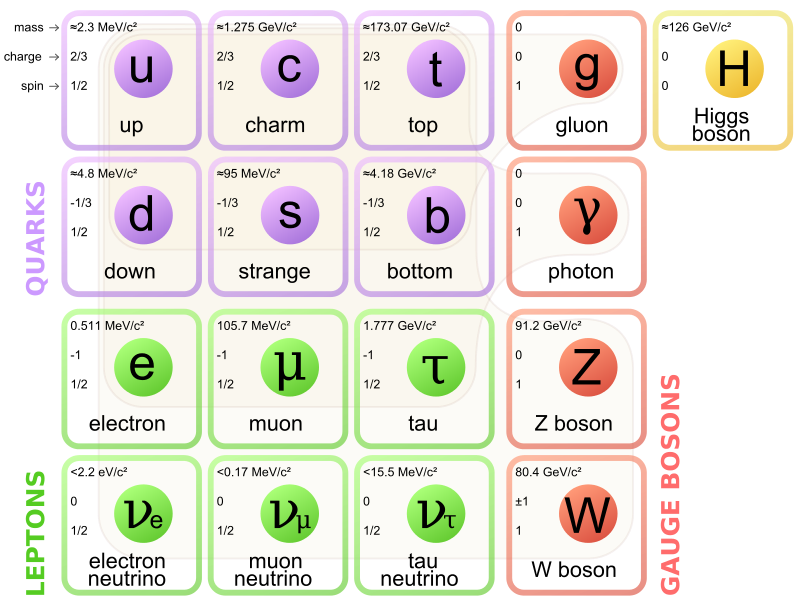
\includegraphics[width=0.8\linewidth]{Figs/Table_of_SM_particles.png}
\caption{\label{fig:standard_particles}
Quarks (purple), leptons (green), and bosons (red and yellow) are shown grouped together by their kind. Anti-particles are not shown. Quarks and leptons stacked above each other have a special relationship via the weak interactions~\cite{wikiparticles}.
}
\end{center}
\end{figure} 

\subsection{Fermions}
Fermions are spin-$\frac{1}{2}$ particles with the Standard Model fermions additionally possessing non-zero charge. The Pauli Exclusion Principle applies to these particles and their corresponding anti-particles. The fermions are further classified by their quantum numbers. The quarks have color and also possess flavor: up, down, charm, strange, top, and bottom. The leptons also have flavor: electron, muon, tau, and the corresponding three neutrinos. The particles exhibiting similar physical behavior are grouped into generations and placed in columns in Fig~\ref{fig:standard_particles} such as up and down or electron and electron neutrino.\\

Quarks primarily interact via the strong interaction with gluons as the force carrier. The theory governing quark and gluon interaction is known as Quantum Chromo Dynamics (QCD) and follows an SU(3) Gauge symmetry and is represented by the T$^a$ group with the following Dirac Lagrangian:
\begin{equation}
\mathcal{L}_{QCD}=i\overline{U}(\partial_\mu - i g_s G^a_\mu T^a)\gamma^\mu U + i\overline{D}(\partial_\mu - i g_s G^a_\mu T^a ) \gamma^\mu D
\end{equation}

They also exhibit a property known as color confinement and thus do not exist as a solitary quark for more than a short period of time. This means that they generally exist in a composite particle with two kinds existing: mesons consisting of two quarks, and hadrons consisting of three quarks. Two well known hadrons are protons and neutrons. The LHC makes use of the collisions of quarks and gluons within the protons as they pass each other in the beam pipe. Quarks also are electromagnetically charged and have weak isospin and hyper charge and thus also interact via the electromagnet and the weak interaction.\\

Leptons are the other SM fermion particles. They do not carry color charge and only interact electroweakly. Electroweak interactions are governed by a Yang-Mills Gauge theory of $U(1)\mathrm{x}SU(2)_L$ given by the following Lagrangian:
\begin{equation}
\mathcal{L}_{EW}=\displaystyle\sum_{\psi} \overline{\psi}\gamma^\mu ( i\partial_\mu - g' \frac{1}{2} Y_W B_\mu - g\frac{1}{2} \vec{\tau}_L\vec{W}_\mu)\psi
\end{equation}
Within the leptons, the neutrinos also do not carry electric charge and therefore do not interact electromagnetically. They only interact via the weak force and thus do not interact very well with our standard matter. Dedicated neutrino detectors are massive and filled with material, yet they still measure very few interactions despite a very high neutrino flux.\\

The fermions are grouped into generations and the masses of each generation are greater than those before it (again, see Fig~\ref{fig:standard_particles} with the left most lepton being the least massive). There are 12 total with all but the first generation able to decay. The first generation makes up the matter that humans interact with every day. Second and third generation quarks are short lived and decay weakly. They are only produced in high energy environments such as those at the LHC. Neutrinos do not decay and very rarely interact with matter.\\



\subsection{Bosons}
 The other types of particles in the Standard Model are bosons. Bosons are most easily differentiated from fermions by the fact that bosons have integer spin and do not follow the Pauli Exclusion Principle. The gauge bosons, that are explained by gauge symmetries in the theory, act as the force carrier that mediates strong, weak, and electromagnetic force interactions. Since it is believed that forces cannot act beyond the speed of light, and QFT requires a field for interactions, gauge bosons are considered to be exchanged between particles as they interact via the fundamental forces. See Fig~\ref{fig:SM_force_mediation} for illustrations of the interactions. The different SM bosons are listed:
 \begin{itemize}
 \item  Photons mediate the electromagnetic interactions between charged particles (for example electron pair production or annihilation) and are often represented with a $\gamma$. Photons are massless and thus propagate at the speed of light. They do however contain momentum equal to their energy. Photons are described by Quantum Electrodynamics which is a subset of the SM.\\
 \item There are three massive gauge bosons: W$^+$, W$^-$, and Z$^0$ with plus 1, minus 1, and neutral electric charge respectively. The W$^+$/W$^-$ are antiparticles of each other while the Z is it's own antiparticle. These particles mediate the weak interaction. The W$^{\pm}$ bosons have a mass of 80.4 \GeVcc while the Z boson has a mass of 90.2 \GeVcc~\cite{pdg}. These bosons decay quickly with the W bosons decaying to two quarks of different flavor and with opposite sign charge or a charged lepton and its corresponding neutrino. The two quarks must be one up-type (up, charm) and one down-type (down, strange, bottom). The W does not decay to the top due to mass and kinematic constraints from the much more massive top quark at current energy accelerators. For the Z boson, the decay must be to a fermion and its anti-particle which in the standard model is quarks and leptons (for example Z  $\rightarrow \ell^+ \ell^- $ where $\ell$ is a charged lepton).\\
 \item Gluons are also massless, electrically neutral particles with spin-1 which mediate interactions between color bearing particles (quarks and gluons). They exist as eight different types due to their color properties. Due to their intrinsic color charge, gluons may self interact. These interactions are described by QCD.\\
 \end{itemize} 
 
  \begin{figure}[h]
\begin{center}
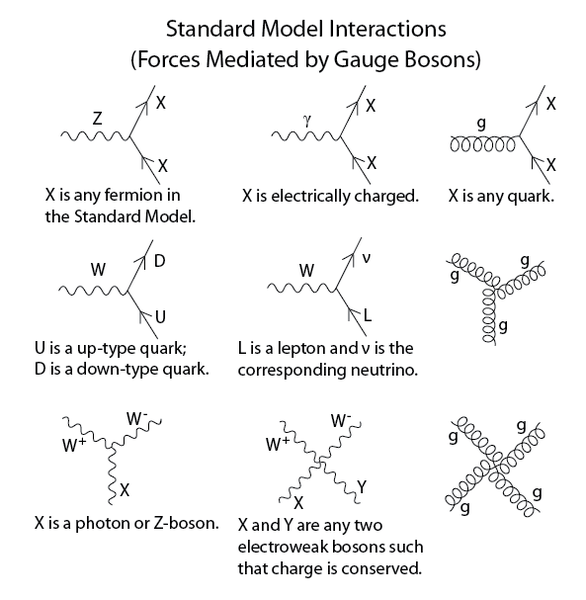
\includegraphics[width=0.8\linewidth]{Figs/SM_force_mediation.png}
\caption{\label{fig:sm_force_meidation}
 The above diagrams represent the various interactions of bosons in the standard model. As noted before a boson is considered to mediate a force between two other particles~\cite{wikimediations}.
}
\end{center}
\end{figure}
 
 The Higgs boson is the last of the standard model bosons. Unlike the previous ones, it is theorized to be a zero spin scalar, which is yet to be fully determined experimentally. It is electrically neutral and color neutral. The current best, and only, measurements come from the LHC and put the mass of the Higgs boson at 125.7 \GeVcc~\cite{discovery, higgstwiki}, which means that it can have self-interactions because it is massive. The existence of the Higgs boson is explained by a theoretical framework known as the Higgs mechanism. This mechanism exhibits spontaneous symmetry breaking and explains why the W$^{\pm}$ and Z are massive while the photon and gluon are not. Additionally the theory can explain the other mass values of the leptons and quarks. Because of the Higgs boson's special relationship with particle mass, it is far more likely to decay to the most massive particles allowed by it's current kinematic energy.\\ 
 
 
 See Fig~\ref{fig:boson_interactions} for the allowed interactions of the various bosons.
 
 \begin{figure}[h]
\begin{center}
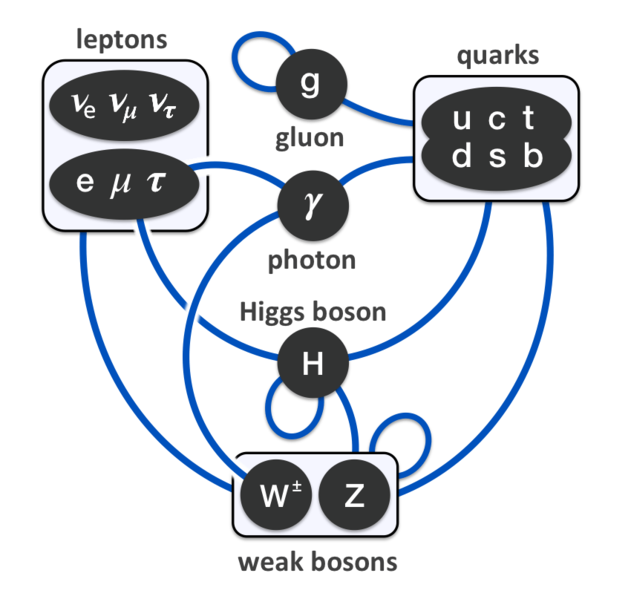
\includegraphics[width=0.8\linewidth]{Figs/particle_interactions_in_SM.png}
\caption{\label{fig:boson_interactions}
 This diagram traces the interactions between various elementary particles in the standard model. It includes self interactions as well. Lines connecting a black oval show interactions between the particles within only the two connected ovals while lines connecting a square show interactions with all of the particles within the square~\cite{wikiinteractions}.
}
\end{center}
\end{figure}

\subsection {Beyond the Standard Model}
Although the Standard Model is both a wildly successful, internally consistent theory and a highly predictive theory for particle interactions, it still is not considered complete. Experimental physics covers two branches with regard to the SM:
\begin{enumerate}
\item Higher precision measurements of known SM phenomena or new measurements of predicted but not yet measured SM phenomena. This is collectively known as SM physics.
\item Attempting to measure ``New Physics" which is physics that is not described by the Standard Model but physicists suspect exist due to deficiencies or perceived weaknesses in the Standard Model. This is primarily known as ``Beyond the Standard Model" (BSM) physics and concerns itself with things like Super Symmetry and Dark Matter.
\end{enumerate}
The topic of this dissertation is a particular Standard Model phenomena, however, the measurements of Standard Model phenomena play into the search for what else may exist that is not covered by the SM as any deviations in SM measurements from theory may provide a clue to new physics. Additionally, experimental confirmation of SM phenomena can provide helpful tools in lowering the uncertainty on BSM measurements. Thus a short explanation of what else may exist is helpful.\\

Some of the major issues with the SM are outlined below:
\begin{itemize}
\item Theories that explain gravitation's source and behavior do not have a SM description.
\item The Standard Model relies on a number of constants that do not have any clear relationship to each other in terms of values. It is considered inelegant to have such a proliferation of components that can only be measured via experiments. A complete theory would hopefully be able to relate the constants to each other mathematically.
\item One conclusion of the SM is that the weak force is much stronger than the gravitational force and leads to an excessive amount of fine tuning. This is known as a hierarchy problem and also manifests itself in the fact that the Higgs mass is many times smaller than the Planck mass. Thus the hierarchy problem is intimately tied to the Higgs mechanism (which doesn't even provide a method to calculate the Higgs mass).
 \end{itemize}
 
 Further, the Standard Model also does not answer some outstanding questions. Thus, although self-consistent, the Standard Model is not a complete description of particle interactions. Some issues are:
 \begin{itemize}
 \item Particle masses and coupling constants take on rather specific values that do not all seem to be mathematically related to each other and have only been measured experimentally. More theory is desired to provide meaningful predictions for these values.
 \item There is a matter and antimatter imbalance in the universe. There is no SM explanation for this. In fact, one would naively assume matter/antimatter to be equally abundant based on the Standard Model.
 \item Some gravitational phenomena have been observed which show that there is far more matter density in the Universe than we can see. This leads to the conclusion that there is some matter than only interacts very weakly with standard matter and has been named ``Dark Matter." There is no explanation for this in the Standard Model.
 \item There is no explanation in the Standard Model for accelerating universe expansion, or the so called ``Dark Energy." 
  \end{itemize}

As said before, these phenomena are not the topic of this dissertation. However, clear and detailed measurements of all of the SM predictions are part of the search for phenomena that are not part of the Standard Model explanation.

	\section{Proton-Proton Collisions} 
	\label{sec:pp_collisions}         
The LHC collides protons with each other at very high energies to study the resulting particles produced and ejected from the collision with the hopes that exotic particles that do not normally exist on Earth will appear briefly due to the high energy in the collision. This makes it a hadron collider. The other main work horse of particle colliders are lepton colliders. Lepton colliders provide very clean events as they only produce final state particles via electromagnetic and weak interactions. However, they are not practical for some studies at very high energies due to the difficulty posed by synchrotron radiation. A lepton collider is usually built linearly to avoid this and thus cannot take advantage of repeated cycles around a ring for continued acceleration or repeated collisions. Thus hadron colliders, though ``messier" in the products that they produce, can provide windows into physical phenomena that are not practical with lepton collisions. Additionally, they open up the possibility of a wide variety of strong interactions.\\

The probability for an interaction to occur is given by the cross section ($\sigma$), which is an analogous way to talk about the ``area" of the particles as they collide. The units typically used to measure this are barns (b) with 1 b = $10^{24}$ cm$^2$.  Due to the size of the protons, number of protons passing each other, and energy of the protons, as well as frequency of production of interesting particles such as bosons, traditionally cross sections at colliders are measured in picobarns ($10^{12}$ b) or even femtobarns ($10^{15}$ b). The average number of collisions in passing particles can be described by the equation:
\begin{equation}
\label{eq:lumi_xsec_relationship}
N = \mathcal{L} \cdot \sigma ,
\end{equation}

where N is the average number of interactions and $\mathcal{L}$ is the instantaneous luminosity (a way of measuring the amount of particles passing each other) which has units of b$^-1$.\\

At the Tevatron, the world's highest energy collider previous to the LHC, protons were collided with antiprotons. However, the LHC decided to use protons only to make production, storage, and accelerating easier~\cite{lhcmachine}. Because at its fundamental level a proton is two up quarks and a down quark (as well as some sea quarks and a lot of gluons), there is an imbalance of initial collision quarks (with up/up collisions being the most likely), whereas at the Tevatron up/antiup collisions were most likely. A typical pp crossing at the LHC has a cross section of $\sigma \approx 100$ mb~\cite{qcdprimer}. Many collisions of this type are elastic, glancing blows between two protons, and thus are not interesting to study. Some are inelastic and cause the production of new particles which are ejected and decay in the detector to study. Because inelastic collisions are between the constituent parts of a proton instead of the proton as a whole, QCD cannot calculate the energies or other meaningful properties of the resulting particles. This is due to the unknown energy and momentum of the constituent partons and how they collide. Over time, experiments have measured the range of probable outcomes of parton collisions and their frequency which can be plugged into several models to extend estimates of the probability of certain types of collisions and kinematics to conditions at the LHC. One such experiment relies on scattering electrons off of protons~\cite{halzen} and measuring the resultant debris to estimate the distribution of energy and momentum of the up, down, and sea quarks, and the gluons. Thus experimental physicists can rely on highly sophisticated Monte Carlo simulations to aid in understanding what to expect from the pp collisions at the LHC.



%	\section{Decays}
%    		(focus on boson decays to quarks and leptons to help motivate the signature later)

\chapter{The Large Hadron Collider and the Compact Muon Solenoid Experiment}
\label{ch:LHC}

The Large Hadron Collider (LHC) is home to several experiments with several thousand collaborators working on them. Work described in this dissertation was performed using data from the Compact Muon Solenoid (CMS), one of the detectors at the LHC. Roughly 3000 collaborators work at CMS alone. The detectors at the LHC are some of the largest and most complicated land-based experimental apparatuses. As such a the following chapter is devoted to describing some of the technical aspects of the LHC and the components of the CMS detector used to measure particles. This will be followed by a description of how the particles are reconstructed and identified (Ch~\ref{ch:particle_reconstruction}). Understanding the functioning of the tools is essential to understanding the results and the methods used to reach them.\\

	\section{The Large Hadron Collider and other Particle Accelerators}
	Modern experimental particle physics relies on two simple ideas, colliding particles together to produce other possibly more interesting or new particles and then measuring these particles directly or measuring their decay products in a large multipurpose detector. Over the years, a large number of experiments have been involved in discovering and confirming most of the particles and properties in the standard model. They have followed a general trend of using either leptons or hadrons to exploit various theoretical properties to produce certain particles more readily, or by ratcheting up the center of mass energy of the collisions from the previous similar experiment (see Figure~\ref{fig:experiment_energies}), or by increasing the rate of collisions in order to collect more data more quickly. Most new experiments rely on some combination of all of these methods to improve over the previous ones and open up new areas of exploration.\\
	
		\begin{figure}[h]
\begin{center}
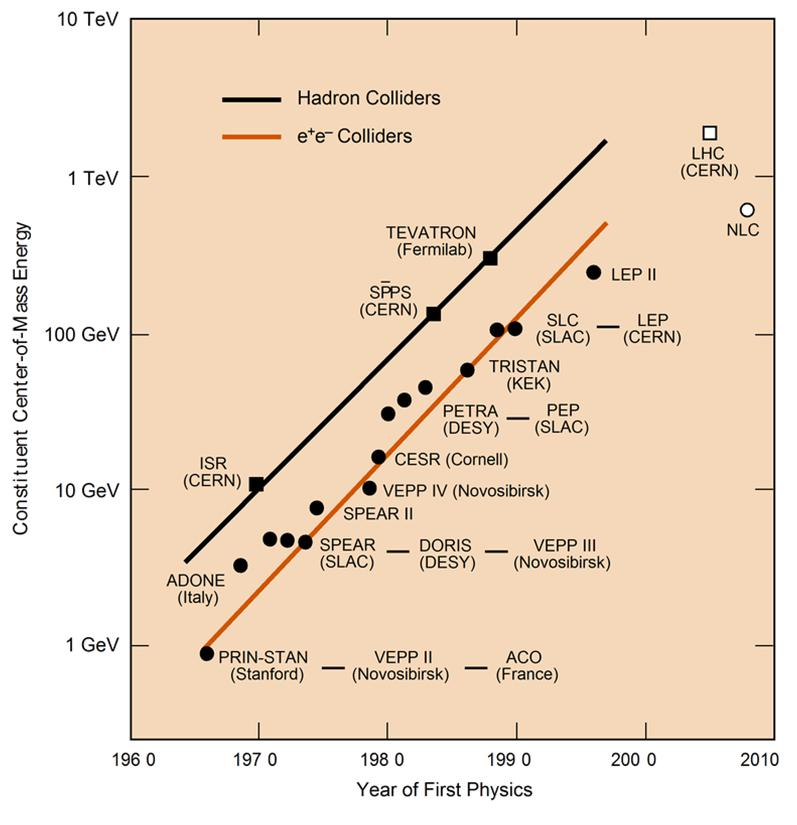
\includegraphics[width=0.8\linewidth]{Figs/collider_energy.jpg}
\caption{\label{fig:experiment_energies}
Plot of experimental accelerator energies and their first year of operation~\cite{comenergy}.
}
\end{center}
\end{figure} 
	
	The Large Hadron Collider (LHC) is the world's current largest and most powerful particle accelerator~\cite{cernlhc}. It is situated at the European Organization for Nuclear Research (CERN) which is headquartered in Geneva, Switzerland, but crosses the border into France. The machine first started up on September 10, 2008 and has collected data periodically since then. The LHC is housed in a 27 km long ring buried underground in which two beams of protons circulate at near the speed of light in opposite directions (see Fig~\ref{fig:lhc_beampipe}). The majority of this ring is filled with superconducting electromagnets to guide the beams, equipment to super cool the magnets to $-271.3^\circ$~C and hold the beam pipes at an ultrahigh vacuum, and other odds and ends to keep the beam circulating. There are 1232 dipole magnets each 15 meters in length to bend the beams and 392 quadrupole magnets  each 5-7 meters in length to focus the beams. By focusing the beams, particles are not lost while circulating and the rate of collision of passing bunches is increased. Collisions occur at the 4 detectors (see Fig~\ref{fig:lhclayout}): CMS, ATLAS, ALICE, and LHCb.
	
	
			\begin{figure}[h]
\begin{center}
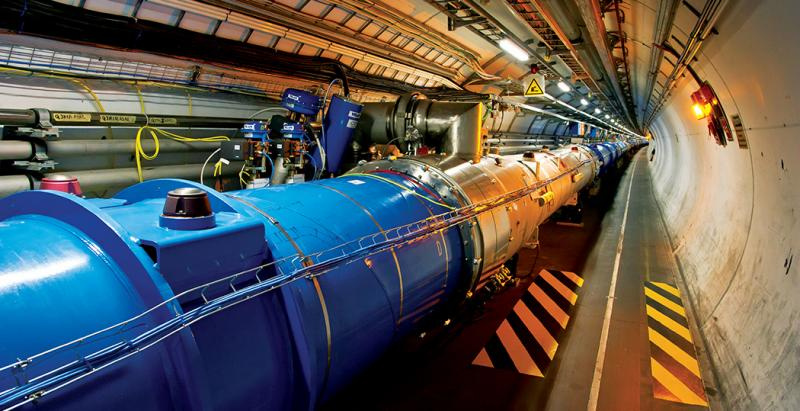
\includegraphics[width=0.8\linewidth]{Figs/lhc_beampipe.jpg}
\caption{\label{fig:lhc_beampipe}
Picture of the interior of the LHC showing the beam pipe and some equipment. Particles circulate around the ring in the very center of this pipe (which is mostly filled with electronics) ~\cite{cernlhc}.
}
\end{center}
\end{figure} 
			

\begin{figure}[h]
\begin{center}
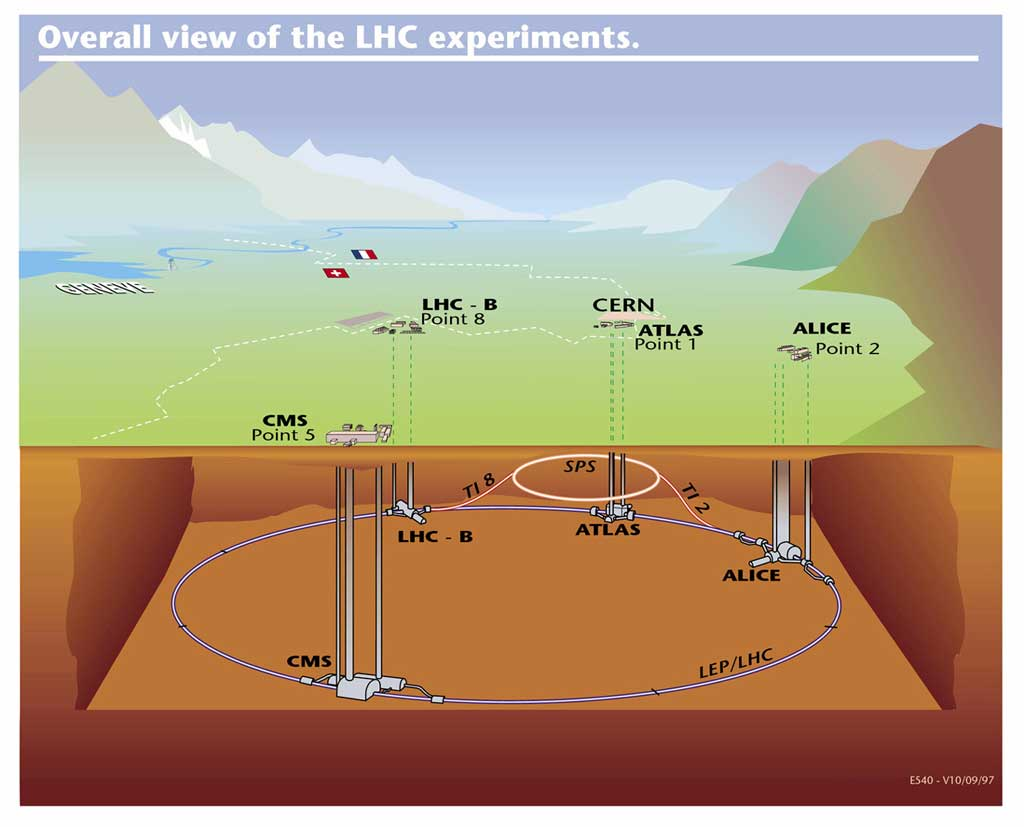
\includegraphics[width=0.8\linewidth]{Figs/lhclayout.jpg}
\caption{\label{fig:lhclayout}
Map of CERN including LHC ring~\cite{lhclayout} with locations of the various detectors.
}
\end{center}
\end{figure} 
	
	
	\section{Description of the CMS detector}        
		The LHC collides protons over 40 million times a second. Most of these are glancing blows, but some are direct collisions that convert some of the extreme energy in the proton momentum into heavy short lived particles that do not usually exist naturally on Earth. The Compact Muon Solenoid (CMS) is one of a few detectors situated at one of the collision spots at the LHC designed to measure the properties of these heavy, short-lived particles and their decay products. Because of the wide range of heavy particles and decay products, CMS is a general purpose detector, designed to measure momentum, energy, charge, and other properties of many different light particles from quarks to leptons to hadrons. The CMS detector is composed of a number of layers that each perform a different role in measurement and combined can paint a very detailed picture of a wide variety of physical phenomena and can be used to reconstruct an entire collision and resulting decays. Once reconstructed, the collision will be a list of particles, there trajectories, energies, and origins. The detector has a coordinate layout in the z-direction along the beam line, measures angles in the xy-plane with an angular variable labeled as $\phi$, and measures angles off of the beam line with the angular variable $\theta$. However, theta is transformed into a Lorentz invariant quantity known as $\eta$ for convenience and is defined as:
\begin{equation}
\eta = -ln [ tan(\frac{\theta}{2} ].
\end{equation}
		
\begin{figure}[h]
\begin{center}
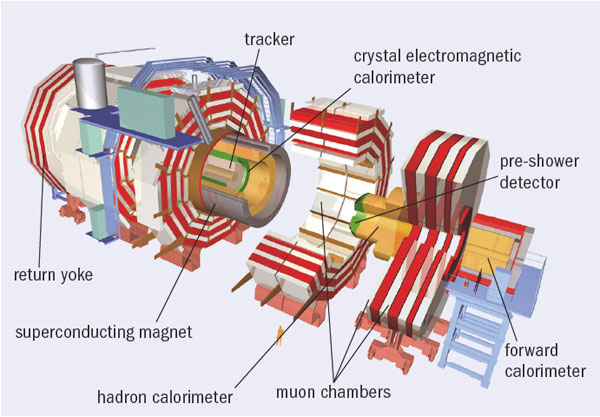
\includegraphics[width=0.8\linewidth]{Figs/cms_detector_internal_clear.jpg}
\caption{\label{fig:cms_internal}
The CMS detector opened up so all layers are visible~\cite{cmspic}.
}
\end{center}
\end{figure} 

		
\begin{figure}[h]
\begin{center}
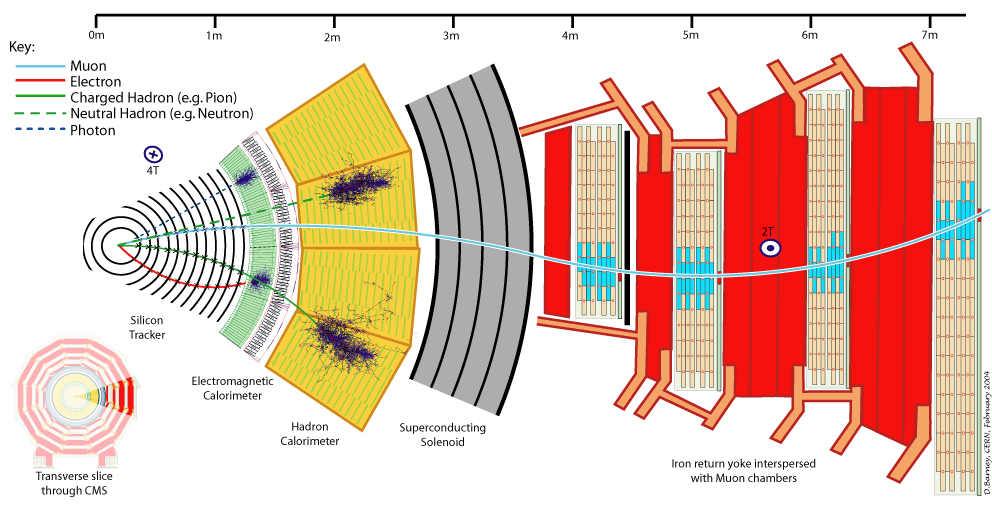
\includegraphics[width=0.8\linewidth]{Figs/CMS_Slice.png}
\caption{\label{fig:cms_slice}
Picture of a cross sectional slice of the CMS detector~\cite{cmspublic}.
}
\end{center}
\end{figure} 

The CMS detector design strives to achieve the following:
\begin{itemize}
\item A high performance system to detect and measure muons (see Muon Detector ~\ref{sec:muon_detector}).
\item A high resolution system to measure the energy and showering shape of electrons and muons (see Electromagnetic Calorimeter ~\ref{sec:electromagnetic_calorimeter}).
\item A high quality system to measure the trajectory of charged particles for accurate momentum measurements (see Silicon Tracker~\ref{sec:silicon_tracker}).
\item A hermetic system that surrounds the collision and fully measures the complete hadronic energy of the event (see Hadronic Calorimeter~\ref{sec:hadronic_calorimeter}).
\item A strong magnetic field to curve the charged particles' trajectories to aid in momentum, energy, and mass measurements as well as identification of the particles' spatial origins (see Solenoidal Magnet~\ref{sec:solenoidal_magnet}).
\end{itemize}

	\subsection{Solenoidal Magnet}
	\label{sec:solenoidal_magnet}
The CMS detector uses a fundamental physical property to help measure momentum: a charged particle's trajectory curves when it travels in a magnetic field. The magnet is a solenoid and just has a field along the Z-axis causing particles to curve in the xy-plane. The solenoid is 13 m long and 7 m in diameter which allows for most of the electronics to be placed inside it. The solenoid is made of a coil of superconducting Niobium-Titanium (NbTi) wire that runs with above 18,000 A of current to create a 3.8 T field storing 2.3 GJ of energy. It is the strongest magnet of it's kind in the world. The magnet strength was chosen to be low enough to allow electrons and other charged particles produced at the lower range of interesting energy to escape the tracker (too strong a field would cause them to curl around inside the tracker) and large enough that very high energy particles still travel with enough curvature that the tracker can somewhat accurately measure the curvature and thus momentum. Given that appreciable curvature must be achieved in roughly 3 meters of travel inside the solenoid, the magnet must be very strong. The magnetic field curves a charged particle with a basic physics property where the force on the charge is given by:
\begin{equation}
\mathrm{\textbf{F}}=q(\mathrm{\textbf{E}}+\mathrm{\textbf{v}}\mathrm{x}\mathrm{\textbf{B}}),
\end{equation}		
where q is the charge, \textbf{E} is the electric field acting on the particle (here it is equal to 0), \textbf{v} is the velocity of the particle, and \textbf{B} is the magnetic field. The particle travels perpendicular to the magnetic field in the transverse plane and thus the curvature of the particle is:
\begin{equation}
r = \frac{\pt}{q |\mathrm{\textbf{B}}|}.
\end{equation}		
		
		
%					\begin{figure}[h]
%\begin{center}
%
\includegraphics[width=0.48\linewidth]{Figs/placeholder.pdf}
%\caption{\label{fig:magnet}
%.
%}
%\end{center}
%\end{figure}

	\subsection{Silicon Tracker}
	\label{sec:silicon_tracker}
	At the time of construction, the CMS silicon tracker is the largest silicon tracker in the world. It is the innermost component of the CMS detector and is used to measure the trajectory of charged particles by measuring the particle's position at discrete location inside the tracker. The silicon tracker is usually discussed as a single measurement device, but is actually made up of two different arrangements of silicon detectors. See Fig~\ref{fig:tracker} for a 2D representation of the tracker layout. The inner area is made of discrete pixels where the occupancy (or flux) of particles is most dense. The outer layer is made of strips where the particles have spread out more (density decreases by the square of the radius from the center). This allows the tracker to save a little on power and readout electronics.The tracker specifications were designed for excellent track trajectory reconstruction, good momentum resolution, and the ability to measure displaced vertices which are used in measurements and identification of heavy particles and b-jets.  However, the enormous amount of silicon, cooling equipment, and readout electronics also comes at a price (other than the very large literal price to build it). The particle resolution is lower than some other style trackers due to multiple scattering of particles as they pass through the tracker as well as lowering the accuracy of energy measurements which have an increased chance to bremsstrahlung and pair create.\\
	
	 The inner area which is closest to the collision and will contain the highest density of particles and thus points of measurement is made out of silicon pixels measuring 100\um by 150 \um. The pixel detectors are made of three barrel layers and two end cap disks. It measures particles to \abseta \lt 2.5 (known as the tracker ``acceptance"). This section also receives the highest dosage of radiation of any of the detector components and must be extremely resilient to radiation. There are 65 million channels of pixels, and thus power consumption was kept to a minimum at 50 microwatts a channel. Even so, the pixels are mounted on cooling tubes so as not to overheat the detector. The silicon tracker exploits a property of silicon where charged particles eject electrons from the silicon atoms as the particles traverse the silicon. Each pixel collects these charges on the surface and measures them as a small electric signal. The pixel spatial resolution in the r-$\phi$ plane is about 10 \um and in the z direction is about 200\um.\\
	
	The outer layer of the tracker does not quite need this level of precision and instead of having pixels, uses less granular "strips" of silicon. This lowers the cost of producing the silicon and even more importantly lowers the amount of readout channels required. Some extra precision is picked up by angling overlapping layers of strips (10 in total) slightly off of parallel to provide a level of stereoscopic location. Thus a rough estimate of which part of a strip the particle passed through can be made by looking at which strip it hit on the next layer.\\
	
	The Silicon strips make up four tracker inner barrel (TIB) layers with two tracker inner end disks (TID), six tracker outer barrel (TOB) layers, and two outer tracker end caps (TEC). The end caps make the pixel detector hermetically sealed, but do not provide the same precision as the barrel track do to a lack of pixels. The TIB and TID have a position resolution of about 23 to 35 \um, and the TOB a resolution of around 35 to 53 \um, and the TEC a resolution of around 97 to 184 \um. Thus most charged particles tend to only considered strongly identified and have well reconstructed momentum if they are picked up by the barrel tracker.\\
	
						\begin{figure}[h]
\begin{center}
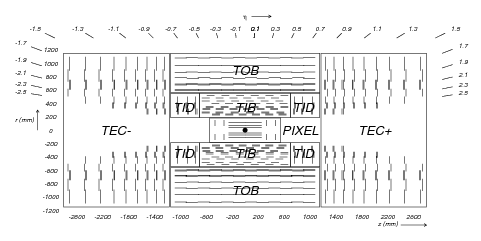
\includegraphics[width=0.8\linewidth]{Figs/tracker_layout.png}
\caption{\label{fig:tracker}
Projection of the tracker in the r-z plane. Modules are shown as lines. Angles are measured in $\eta$~\cite{trackingperformance}.
}
\end{center}
\end{figure}
	
	\subsection{Electromagnetic Calorimeter}
	\label{sec:electromagnetic_calorimeter}
	Once a particle's trajectory has been measured in the tracker (with minimal energy loss), it is time to measure the particle's total energy as well. This step must be done second as measuring the energy of a particle is messy requiring collisions with a material that will alter and stop the particle's movement. The calorimeters at CMS are designed to be hermetic, meaning they are designed to fully contain all of the energy from quarks, electrons, and photons to facilitate the measurement of non-interacting parcels like neutrinos by measuring the momentum imbalance in the detector. The CMS detector additionally exploits the fact that different particles interact with different material at different rates. Thus a calorimeter can be designed to primarily measure the energy of electromagnetic particles such as electrons and muons while letting hadronic particles (quarks) mostly pass through to the next layer. This helps both with energy measurement as well as identification. At a very reduced level of complexity, electrons have a track in the tracker and leave a large amount of energy in the Electromagnetic Calorimeter (ECAL) and little to no energy in the Hadronic Calorimeter (HCAL). Photons are similar but being neutral do not leave tracks. Quarks, charged mesons, and jets have tracks and leave some energy in the ECAL and deposit the majority of the energy in the HCAL (see Sec~\ref{sec:hadronic_calorimeter}).\\
	
	The ECAL is made of lead tungstate (PbWO4) crystals that are very dense with a radiation length of 0.89 cm and a Moli\`{e}re radius of 2.2 cm. With oxygen added into the crystals, they are relatively transparent to light, and scintillate (release a large amount of photons) when an electron or photon pass through them. This scintillation is immediate, short lived, and well-defined by the incoming particle's energy. The crystals are very resilient to radiation and thus have a long operational life. The ECAL is compact and accurate at measuring energy at the frequency of collisions at the LHC. In the barrel, the crystals measure 2.2 x 2.2 x 23 cm and 3 x 3 x 22 cm in the end caps with a total of 75,848 crystals in the ECAL. Note that the crystals are intentionally about the same size as 1 Moli\`{e}re radius so that a single crystal will contain most of the energy spread of an interacting electromagnetic particle. The crystals were grown to exacting standard to produce to achieve a high level of homogeneity. There is additionally a pre-shower system which helps crudely measure the trajectory of the particles after leaving the tracker (useful for determining the photon trajectory and matching electron showers to tracks). The ECAL barrel measures particles with pseudorapidity up to \abseta \lt 1.479.\\
	
	The ECAL end caps also contain and additional 7324 PbW0$_4$ crystals and cover the pseudorapidity range f 1.479 \lt \abseta \lt 3.0. This leads to a slight crack in coverage between the barrel ECAL and the endcap ECAL. Generally electromagnetic particles that cross through this track are not used in measurements where accurate momentum measurements and particle identifications are needed. The crystals in the endcaps are approximately 30x30 mm with a length of 220 mm. They are oriented so that the 30x30 mm surface faces the collision point and electromagnetic particles will travel the length of a crystal as it traverses the detector.
	 
	 
						\begin{figure}[h]
\begin{center}
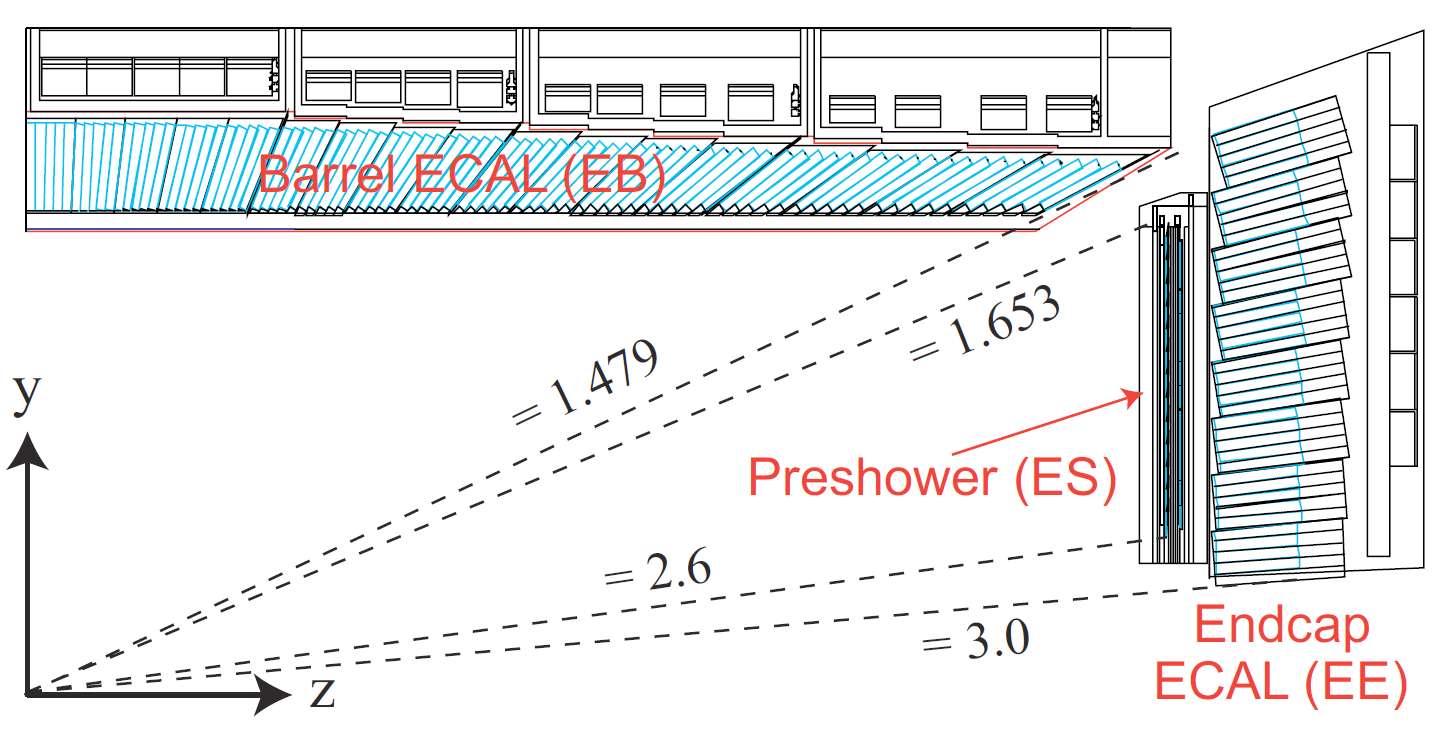
\includegraphics[width=0.8\linewidth]{Figs/ECAL_layout.png}
\caption{\label{fig:ecal}
The crystal layout of ECAL by pseudorapidity range~\cite{tdr1}.
}
\end{center}
\end{figure}
	
	\subsection{Hadronic Calorimeter}
	\label{sec:hadronic_calorimeter}
	The Hadronic Calorimeter (HCAL) uses a different set of materials with different interaction properties to stop and measure the energy of hadronic particles which are made of quarks and gluons. This layer is outside the ECAL and thus measures very little energy from electromagnetic particles such as electrons and muons. The HCAL is hermetically sealed so that it should measure all of the energy in the collision that has not already been measured by the ECAL. Notable exceptions include muons which get measured in the Muon Chamber and weakly interacting neutral particles such as neutrinos (or possible Super Symmetric particles). The latter weakly interacting particles can be inferred by a momentum and energy imbalance thanks to the hermetic properties of the detector and the conservation of energy.\\
	
	The HCAL is a sampling calorimeter structured with alternating layers of absorbing material  which causes incoming particles to shower and scintillators which produce light when the showers pass through. The scintillator light is amplified by photodetectors. Each layer can record position, energy, and time of arrival. Sections of radial layers are grouped together to form a ``tower," and the towers are used to determine the total energy and the direction of travel of the particle that produced it by grouping energy filled towers together that are near each other.\\
	
	The overall HCAL consists of a barrel (HB) section assembled from 36 wedges, an endcap (HE) section also made of 36 wedges, and forward (HF) sections which pick up particles that come out at very shallow angles to the beam line. There is an additional section (HO) outside the barrel and the magnetic coil. The full layout of the HCAL can be found in Fig~\ref{fig:hcal}.\\
	
						\begin{figure}[h]
\begin{center}
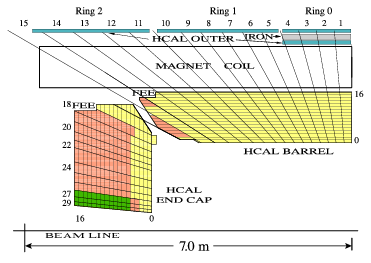
\includegraphics[width=0.8\linewidth]{Figs/HCAL_layout.png}
\caption{\label{fig:hcal}
Map of the HCAL layout flattened into r-z space~\cite{hcalperformance}.
}
\end{center}
\end{figure}

The HB and HE use brass alloy as the absorbing material to ensure the majority of hadronic particles shower in the HCAL. In places the HB is over 10 interaction lengths thick. The HB covers up to \abseta \lt 1.3 with a spacial segmentation of 0.087x0.087 in $\eta - \phi$ space. Between 1.3 \lt \abseta \lt 3.0 with a resolution that is the same as the ECAL until \abseta \lt 1.6 where it becomes 0.17x0.17 in $\eta - \phi$ space. Between 3.0 \lt \abseta \lt 5.0 coverage is picked up by the HF which uses steel as an absorber. The scintillators were replaced with hard quartz fibers which rely on Cherenkov radiation in order to cope with the much greater occupancy at this closeness to the beam pipe. The resolution here is about 0.18x0.18 in $\eta - \phi$ space. Finally, in order to catch particles that pass through the HB, the HO uses the solenoid magnet as an extra layer of absorber. The HO is just another layer of scintillators which sit outside the solenoid. All of this material reaches almost 12 interaction lengths and makes the probability of a hadronic particle reaching the muon detector to be \lt 0.1\%.
	
	\subsection{Muon Detector}
	\label{sec:muon_detector}
	Muons are charged leptons like electrons, so they leave a track in the tracker. Unlike electrons, muons interact somewhat weakly and thus do not shower in the ECAL or HCAL. Because of their ability to pass through several meters of iron and travel relatively far before decaying, there is a special section to measure muons which is placed on the outside of the detector after all of the other particles should have showered and been stopped by the two calorimeters and the iron return yoke. \\
	
	Within the Muon Detector, there are 1400 chambers: 250 drift tubes (DTs) which for a cylindrically concentric sub-detector, 540 cathode strip chambers (CSCs) (for position measurements and triggering) that form four layers on each side of the barrel, and 610 resistive plate chambers (RPCs) (as a redundant triggering system). The DTs and RPCs are arranged in concentric cylinders around the beam line while the CSCs and RPCs make the disks that cover the ends of the cylinder. The layers are interspersed with the iron return yoke which further helps to act as an absorber to filter out any non-muon particles that made it through the calorimeters.\\
	
	The muon detector consists of four layers each divided into smaller modules known as ``stations." The layers are separated by iron which is part of the return yoke. Because the muon detector is located outside of the solenoid, the return yoke helps to create a magnetic field in the opposite direction of the field inside the solenoid, thus when the Tracker and Muon Detector show the trajectory of a muon, it looks like an 'S.'\\
	
	The Muon Drift Tubes are 4 cm wide tubes which contain a wire stretched down the length of the tube and a gas that is prone to losing electrons as charged particles pass through it. A voltage is applied across the wire and thus knocked off electrons are collected at the positive end. Using the amount of charge collected, the distance of closest approach to the wire can be calculated. Using the amount of time it takes to move the charge down the wire to the positive end, the distance position along the wire's axis can be determined for the muon's approach. Thus each tube can give a two dimensional position measurement of the muon. To make a DT chamber, 60 DTs are collected into 12 layers arranged in three groups of four. The DT chambers average 2mx2.5m in size and multiple DT chambers surround the detector. They cover a pseudorapidity range of up to \abseta \lt 1.2. They also give a spatial resolution of 100 \um in the r-$\phi$ plane with 25 ns timing.\\
	
	The CSCs are composed of overlapping and perpendicular copper cathodes and anode wires. Between the two layers is a gas. Electrons from the gas are collected on the anodes and ions (now missing an electron) are collected on the cathodes. The anode wires run along the azimuthal direction and provide the radial measurement while the strips run lengthwise in a radial direction and give  $\phi$ measurement. This a very fast system and thus is suitable for triggering. They cover a region of 0.9 \lt \abseta \lt 2.4. Just like the barrel, there are four stations. They are arranged in radial disks perpendicular to the beam line. It has a measurement resolution of between 75 and 150 \um.
	
	RPCs work similarly to the CSCs but instead have two parallel plates made of a highly resistive material. Strips outside the plates pick up the presence of the charged particles. RPCs have good spatial resolution and time resolution down to one nanosecond which also makes them excellent for triggering. Their primary purpose is to enhance the timing resolution of muon measurements, since their spatial measurements (though accurate enough for triggering) are not as accurate as the spatial measurements of the other sub-detectors in the muon detector while their timing resolution is well below the 25 ns maximum collision rate.\\
						\begin{figure}[h]
\begin{center}
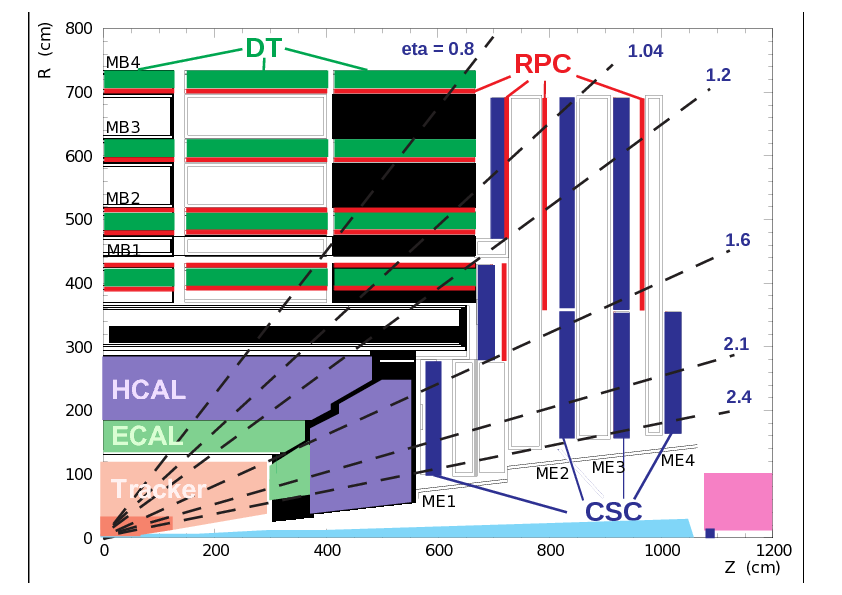
\includegraphics[width=0.8\linewidth]{Figs/muon_system.png}
\caption{\label{fig:muonchamber}
Layout of the CMS muon system with sub-detectors in projected in r-z plane. The Drift Tubes (green), the Cathode Strip Chambers (blue), and the Resistive Plate Chambers (red) are shown~\cite{muontdr}.
}
\end{center}
\end{figure}
	
		The muon system overall was designed close to 95\% efficiency with less than 10\% resolution for muons with \pt = 200 \GeV. Once combined with the tracker, this reduces the resolution to 1\% for lower \pt muons and 5\% for those even up to \TeV range.\\
		
		
		
	
	\section{Luminosity Measurement}	
		Luminosity is defined as the ratio of the number of particles detected (N) in a certain time (t) to the interaction cross-section ($\sigma$). 
		\begin{equation}
		\mathcal{L} = \frac{1}{\sigma} \frac{dN}{dt}
		\end{equation}
		
		The relationship between luminosity, cross section, and number of collisions was expressed early in another form in Equation~\ref{eq:lumi_xsec_relationship}. The form above expresses the luminosity in terms of an instantaneous value whereas the useful form for particle physics is integrated luminosity, which as the name implies is the total luminosity over time and not just at any given instant. Luminosity can be thought of conceptually in a naive analogy with light. If one turns on a light in a room, there is some level of luminosity which correlates to the number of photons per second leaving the light bulb. The more luminosity the bulb provides, the more light will scatter off of objects and return to the person's eye and the better the person can see the surrounding area. In particle physics, luminosity correlates to the amount of collisions that can be produced with any given cross section. If one provides fixed objects (such as protons) then the cross section is also fixed, and thus the only way to increase the number of collisions is to increase the luminosity, which among other things depends highly on the number of particles passing in close proximity to each other per unit time. \\
		
		Up to the end of data taking in 2012, the LHC delivered an integrated luminosity of 23.3 \fbinv. Of collisions produced, CMS was able to record 21.8 \fbinv and due to various transient issues, was able to certify 19.5 \fbinv of integrated luminosity as ``good" data that could be used for measuring physical phenomena. The uncertainty on this measurement was 2.6\%~\cite{lumi12up} and contributes to the total uncertainty of any measurement conducted with CMS data. Figure~\ref{fig:cms_int_lumi} shows the integrated luminosity produced by the LHC and measured by CMS over time.\\
\begin{figure}[h]
\begin{center}
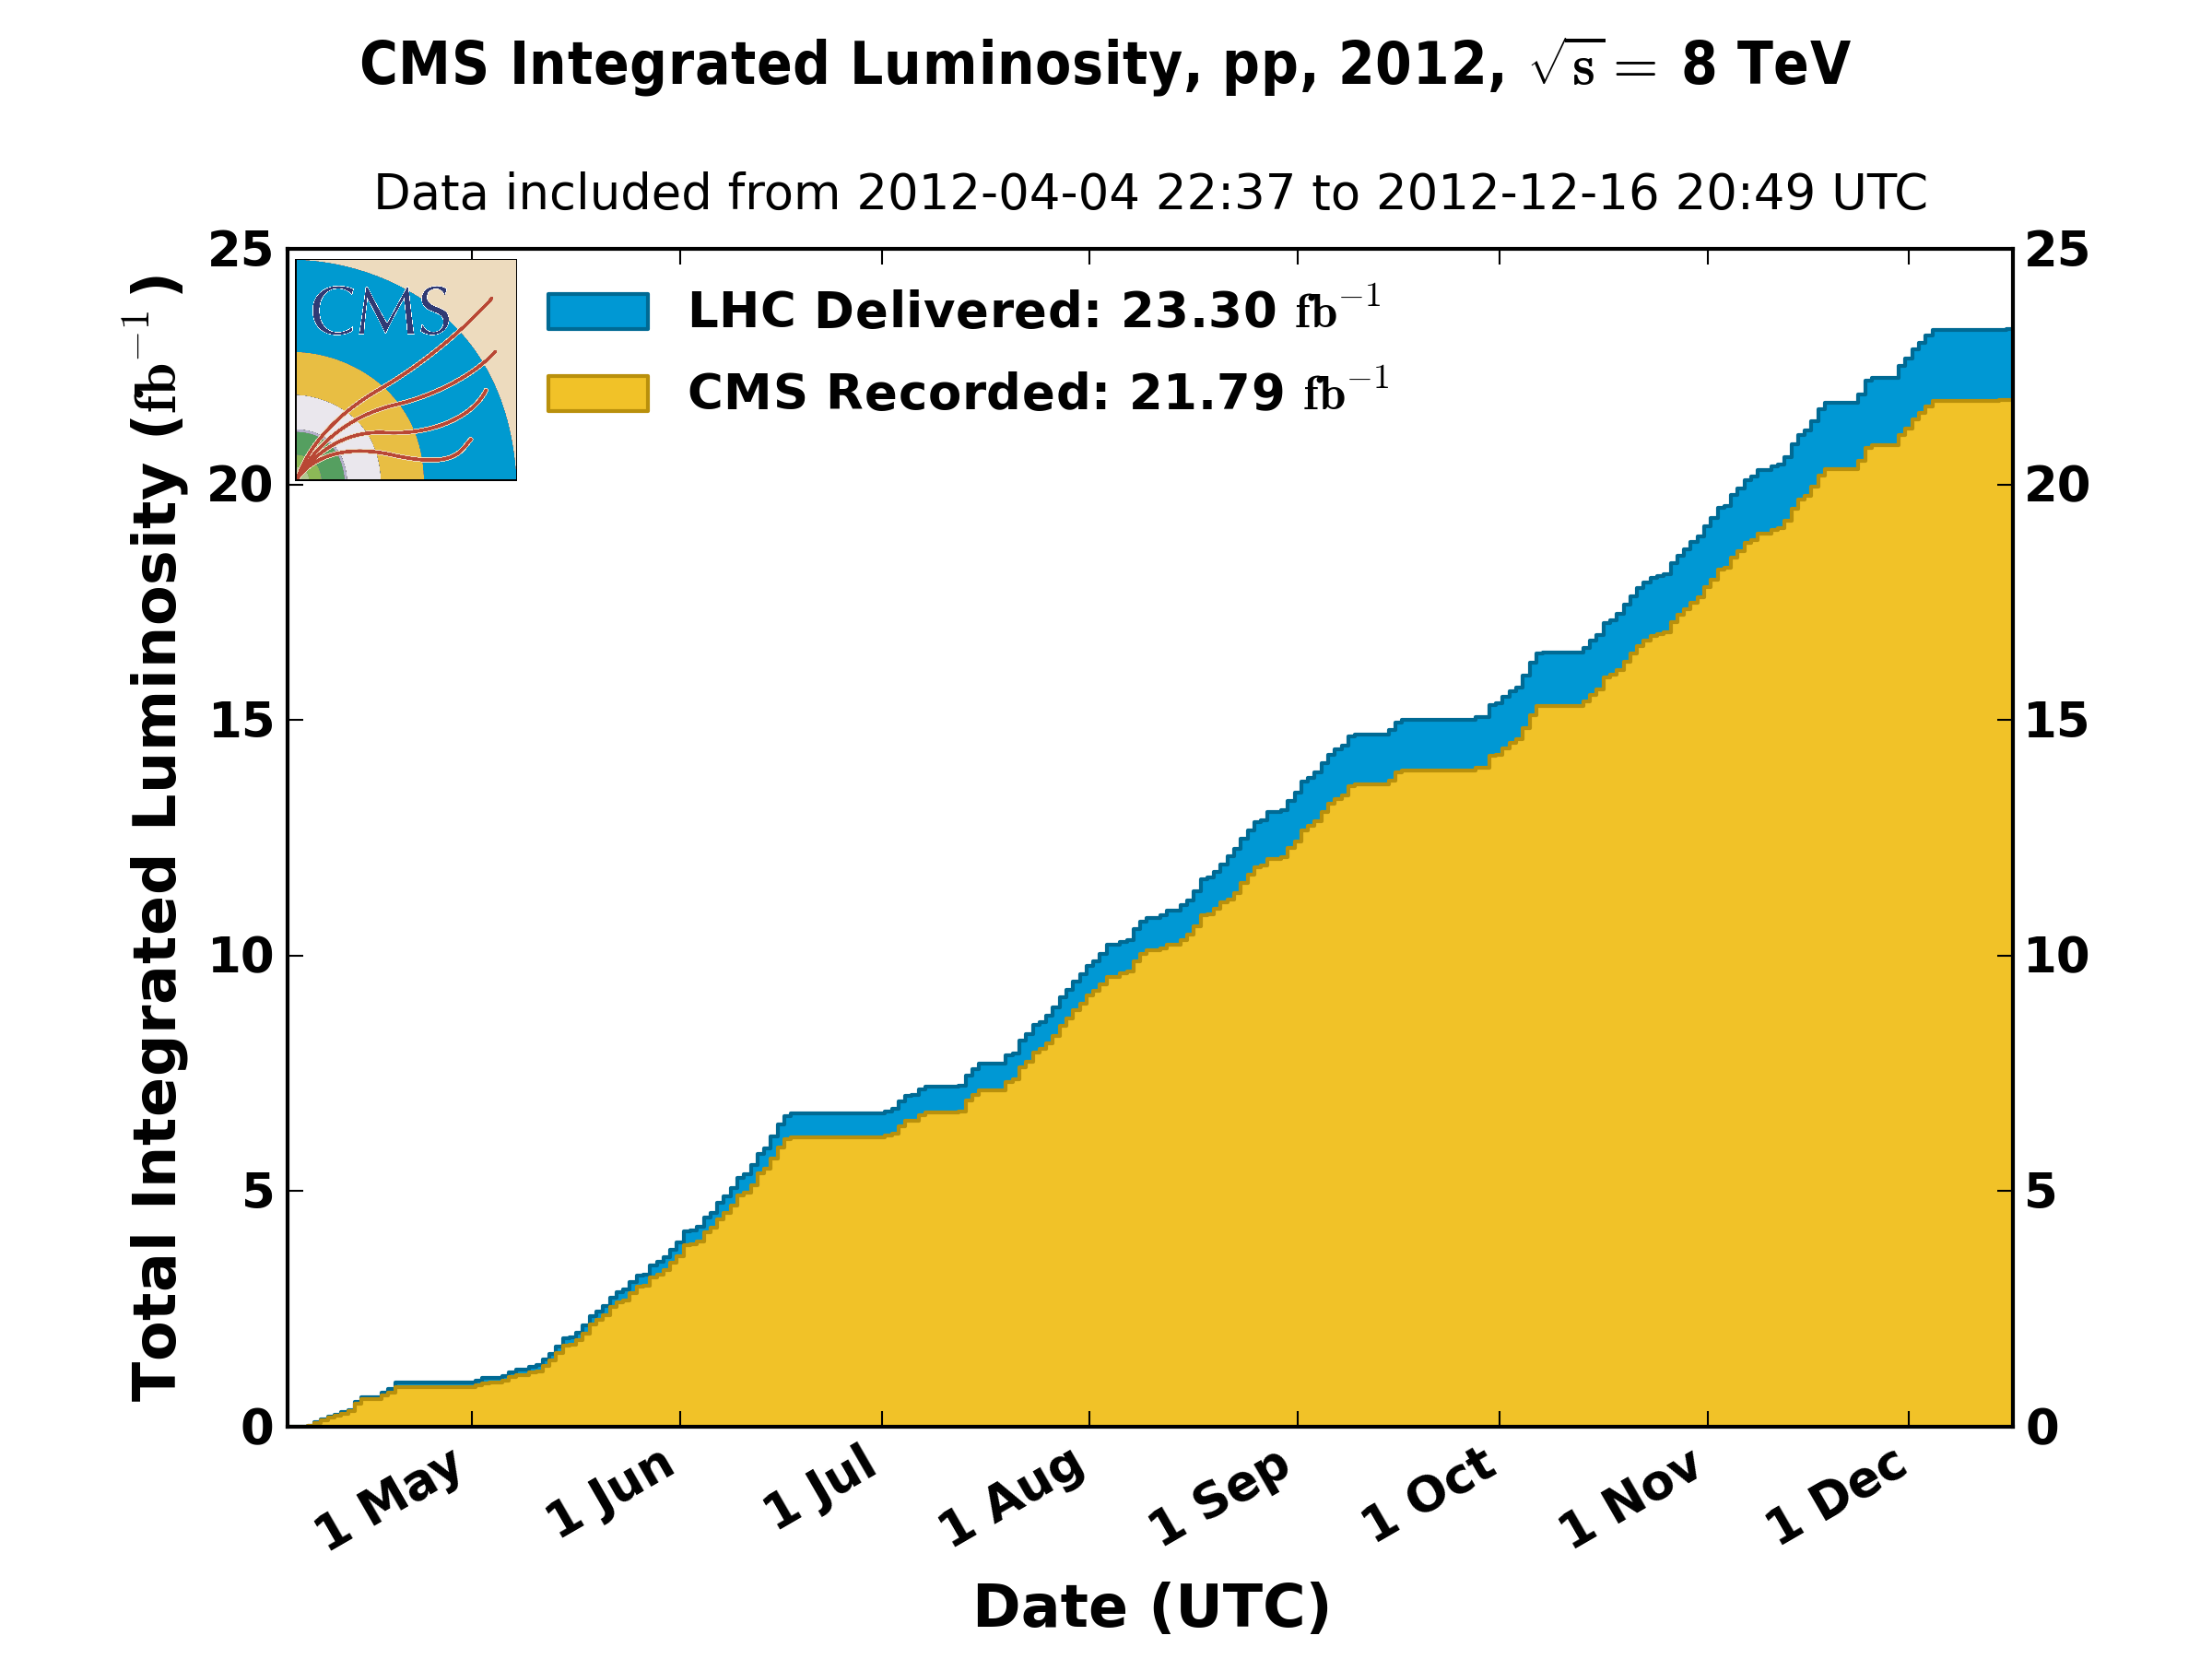
\includegraphics[width=0.9\linewidth]{Figs/int_lumi_per_day_cumulative_pp_2012.png}
\caption{\label{fig:cms_int_lumi}
Plot of 8 \TeV data collection over time. The delivered data (blue) is slightly above the recorded data (yellow) as the detector is not able to record every collision due to various transient issues.
}
\end{center}
\end{figure}

The luminosity at CMS is measured using two methods. The first method is the original method and the second is somewhat newer. The first relies on the HF calorimeters which are very far forward at $\abseta \gt 3.0$, which is well beyond the range of the tracker. When triggering on zero-bias events with random triggers that are agnostic of activities inside the detector, a measurement of the average fraction of empty calorimeter readouts is then converted into a cross section and used to measure instantaneous luminosity~\cite{lumi11}. This method, however, has a problem due to the non-linear response in the HF as a function of instantaneous luminosity.\\

Thus the second method was produced which relies on the fine granularity of the pixel detector~\cite{lumi12}~\cite{lumi12up}. There is an incredibly unlikely chance of multiple particles leaving a deposit in the same pixel ($\sim$ 0.1\%), and thus the number pixel clusters activated during a bunch crossing can very accurately be related to the proton-proton cross section and thus converted into a luminosity measurement.\\
				
	\section{Triggering}       
	When operating at full design specification, bunch crossings (and thus particle collisions) are occurring at a rate of 40 GHz (for a crossing every 25 nanoseconds). This rate is far too high for electronics to read out data from every bunch crossing and would create an impossibly large amount of data to store and use ($\sim 10^4$ times more data than can be written to disk). The rate collision rate must be high to because events that contain useful standard model processes such as boson (especially multi-boson production) and top production are rare, and ``new physics'' production (such as SUSY production) is even rare still, if it even exists at all. This allows for a scheme of throwing away the large percentage of data early on that would be rejected upstream anyway by the physicists who use it for research.\\
	
	The scheme for filtering collisions is known as ``triggering''~\cite{triggertdr1}. CMS is unique amongst detectors in recent history in that it uses a two level scheme, while others such as at Zues and the Tevatron used a three level scheme. Even ATLAS, the other multipurpose detector at the LHC, also uses a three level system. At the time ATLAS was first being designed, and at previous experiments, telecom switches did not exist that could carry the full 100 kHz output of 1 mb events directly to a computer farm. The three level system had a first level implemented in hardware to choose events in the detector (L1) and then a second also implemented in hardware (L2) to further reduce the rate before transfer away from the detector to the computer farms for software triggering (L3) which could implement more advanced decisions.\\
	
	CMS began design shortly after ATLAS and benefitted from more knowledge to predict future hardware trends. The design called for two trigger levels: one at hardware level (L1) which reduces the rate from 40 MHz to 100 kHz, and one at software level (L2). See Fig~\ref{fig:trigger_chain} for a simplified representation of the trigger chain. This has the benefit of allowing for less restrictive triggers that can make more complicated decisions without losing potentially useful events through too crude of a filter. The L1 trigger makes use of only muon data calorimeter data (in a fairly raw form without advanced processing) to decide on whether to keep the data and push it into the pipeline for compression and transfer to the L2. The L2 uses all the available data coupled with sophisticated reconstruction algorithms. These algorithms, however, are still much simpler than the same (and similar) ones used with data processing and particle reconstruction later on by the physicists to analyze the data.\\
	\begin{figure}[h]
\begin{center}
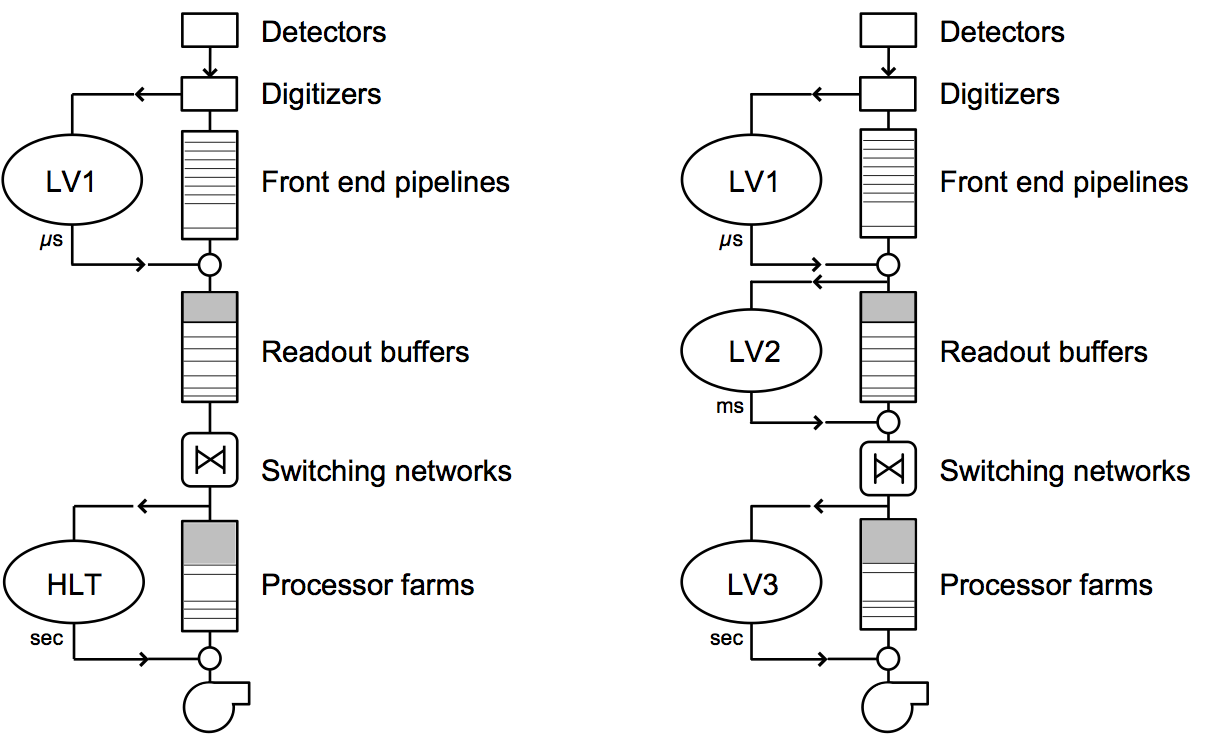
\includegraphics[width=0.9\linewidth]{Figs/2level_3level_trigger.png}
\caption{\label{fig:trigger_chain}
Schematic of triggering for two level and three level systems. Left: CMS method with a single High-Level Trig-
ger (HLT) providing all filtering after the Level-1 decision. Right: the HLT performed in two stages (L2 and
L3)~\cite{triggertdr1}.
}
\end{center}
\end{figure}

	
	Triggering is a very successful way to reduce the rate of data from the detector, but does have a downside. Although the two level system allows for a great deal of flexibility, the hardware triggers are set before runtime. The software triggers are also not changed frequently for a consistent set of decisions to determine the events that are kept. Thus for periods of runs, the triggers are largely static. This creates a difference between algorithms used to reconstruct quantities (such as counting energy in a cone around a particle) at trigger level (``online'' decisions) and similar algorithms used to reconstruct the same quantities at analysis time (``offline''). Care must be taken to require the online algorithms to be a complete subset of the offline algorithms to prevent unintended shaping of the data. Thus if a trigger requires an electron with a maximum amount of energy in a certain sized cone around the electron, this requirement must also be enforced by the physicists analyzing the data. Triggering also produces a very small amount of uncertainty that must be measured and included in the final tabulation of uncertainty on any measurement.\\
	

\chapter{Particle Reconstruction}
\label{ch:particle_reconstruction}
	The detector does not actually measure a "particle" but merely it's presence at certain locations and energy at certain points in the detector. This information is an overwhelming mix of pixel hits, tracker hits, ECAL tower deposits, HCAL deposits, and Muon chamber hits. The raw data is nothing more than thousands of locations, times, and energy deposits. Very sophisticated software is used to connect the dots and of the hits in the tracker into likely trajectories, cluster recordings of energy in the Calorimeters into likely deposits from a showering particle, and connect muon chamber hits into another trajectory. These various pieces of information are then sewn together to reconstruct the full trajectory and energy of particles and apply a likely identification. The following sections outline the various strategies employed to identify and reconstruct information about the particles in the detector.\\	
	
	
	\section{Charged Particle Reconstruction}
	\label{sec:charged_particle_reconstruction}
	The CMS Tracker is designed as the primary measurement device for the trajectory of charged particles. Here, they leave thousands of ``hits" in the pixels and strips to mark their passage. Sophisticated algorithms use an iterative pattern recognition to assemble tracks starting from the center of the tracker. A charged particle moves in a helical trajectory (curved in the XY-plane and straight in the Z-axis). A helix is described by 5 parameters and as such the tracking algorithm starts with a very crude estimate of the parameters and searches for further hits that could match a track with those parameters, and does this layer by layer~\cite{pixel, mangano, trackingperformance}.\\
	
	There are a few variations on the tracking algorithm designed to help identify a few fringe cases, but the primary one which identifies the majority of the tracks is as follows. Hits in the inner most layers are clustered together into what is known as a ``seed." A seed has enough data (usually 3 hits, but some seeds with 2 hits are used) so that it can give a starting estimate of a particles trajectory and an error on that trajectory. The beam collision spot is also used to help determine the particle's trajectory from the seed. The seed is then used as the starting point for a combinatorial Kalman filter~\cite{ckf} which takes the trajectory estimate form the seed and looks to the next layer for a hit within a certain window of error. If it finds a hit that is consistent, then it creates a track candidate of the seed plus hit, refines he trajectory estimate and associated error, and then attempts to find a hit at the next layer. The algorithm can be tailored to look for different particles. For example a muon does not interact very much with the detector and therefore travels on a smooth trajectory. Thus muons could be searched for with a smaller window. On the other hand, an electron scatters a lot and radiates photons and therefore does not follow a very smooth trajectory. Instead it has a certain amount of random (and somewhat well quantified) random motion that can be accounted for by strategically enlarging the window to a proper size. The algorithm also employs other tricks that are often particle specific to account for multiple scattering and energy loss within the detector.\\
	
	If a hit is not found in one layer, the filter will widen the window and jump to the next layer. Although eventually tracks may be built up missing some hits in various layers, these are generally not seen as high enough quality to be used for identifying leptons, but they are occasionally still useful for something and thus are kept. Another possibility is that more than one hit may be found that falls within the window. At this point the algorithm ``branches" the track candidate into two track candidates, one containing each potential hit. In the end the one with the most total hits and the best final fit on the trajectory is kept. When tracks candidates overlap, only one is kept in the final track collection.\\
	
	Once the initial track candidates are found, they are fit with a helix. The best candidates are kept where best usually requires very few missing hits and a low error on the fit. The hits in these tracks are removed from the hit collection, and the other variations on the tracking algorithm pick through the remaining hits to find more tracks. These tracks are less likely to be as high quality as the initial group, but they are still useful and can often help in determining a charged particle's identity.\\
	
	Seeding is also performed several times using different algorithms to determine the seeds. Seeds are basically collections of 2 or 3 hits. Most of the time they are in the inner 2 or 3 layers of the tracker, but some seed algorithms that are used later will also use the 2 or 3 outer layers. There are 7 seeding steps with the ones applied earliest most likely to lead to a true particle track reconstruction. The first two steps use a hit triplet from the inner layers with the most stringent seed also containing a minimum \pt cut on the particles momentum. The second one drops the \pt cut. The third step uses a hit doublet in the inner layers for additional efficiency. The fourth step is similar to the first step however it lowers the compatibility of the hits with the interaction point in order to search for tracks with displace vertices and or tracks that came from particles with longer lifetimes. The fifth step requires 3 hits again, but allows for them to be comprised of hits from both the pixels and the strips to allow for seeding of particles with a missed pixel hit or longer decay lengths. That last steps use pairs and triplets of hits on layers farther away from the center of the detector to find tracks of particles with a large displacement from the interaction point.\\
	
	After each step in the seeds have been propagated through the Kalman filter and associate propagation algorithms, the track candidates are fit for a final trajectory. Hits that fall too far from this trajectory are removed from the track. The 5 track parameters and associated errors are pulled from the final fit. Quality of the track is determined by things like vertex compatibility, number of hits in the track, and the $\chi ^2$ of the fit. As stated before, hits from tracks that are of a high enough quality are removed before the next step begins. In the end, all identified tracks from the seven steps are merged into one collection and for any tracks that overlap for a high enough number only the best candidate is kept.\\
	
		
	\section{Vertex Reconstruction}
	When an event passes a trigger, that usually means that there is some high \pt particle present in the event. This particle came from the interaction of two protons. However, for every proton-proton collision that produces an interesting particle, there are tens more in the same bunch crossing of protons that produced low energy particles that are not interesting. Particle reconstruction and measurement relies very heavily on knowing the location of the collision vertex and thus a good method for differentiation this must be used. Some examples of how knowing the accurate location of the vertex can help are: understanding the lepton impact parameter to reject muons that came from semi-leptonic decease (and thus will have a displaced vertex from the collision vertex), or identifying electrons that came from photon conversions.\\
	
	To find the vertices of the bunch crossing, first, tracks are clustered using a deterministic annealing algorithm~\cite{davtx, dacms}. Deterministic annealing algorithms have a high clustering efficiency in noisy environments like the LHC, with a vertex efficiency with a linear response function to the number of interactions. The algorithm is another iterative algorithm that clusters tracks with nearby impact parameters. It starts with large windows for the proximity of the impact parameters and tightens the window for each iteration until a stop condition is met. If a track has a transverse impact parameter \gt 3 cm or a longitudinal impact parameter \gt 4 cm it is not used in the clustering.\\
	
	Next, each cluster of tracks is used to fit a vertex position for the tracks using an adaptive vertex fitting algorithm~\cite{vertexing,vtxfit}. Tracks in the cluster that are more compatible with a vertex position for the cluster are weighted more heavily which gives a good vertex resolution of less than 50 $\mu$m (with variations in accuracy depending on the number of present tracks).\\ 
	
	
	\section{Electron Reconstruction}
	Electrons are produced in a variety of ways, but primarily the decays of interest are from bosons. This produces isolated electrons, meaning they are spatially separated from other particles in the detector. This helps in electron reconstruction, but other electron characteristics make identifying the electron harder. Electrons multiply scatter more than other particles in the tracker, radiate photons via bremstrahlung, and generally interact electromagnetically with the material they pass through. This leads to several challenges in reconstruction, on of which is a highly spread out energy distribution in the detector (both radially and angular). The main source of energy measurement for electrons is the energy deposited in the ECAL. However, this also becomes tricky to disentangle the electron energy from other deposits such as those from $\pi ^0$ which decay to photons or other hadronic particles which still start to shower in the ECAL. Thus electron identification has a goal of not only reconstructing electrons and their energy accurately, but also attempting to decide which ones originated from the proton interaction (such as electrons from boson decay) and which ones were produced later on. Details on the reconstruction of electrons, their trajectory, and their energy are discussed below while details of identifying electrons specifically from boson decay are discussed in Sec~\ref{sec:ElectronSelections}.\\
	
	Electron reconstruction is a complicated procedure and a great deal of details beyond the summary provided here may be found in~\cite{baffiReco,egmReco,egm201}. The naive picture of an electron in the detector is a particle that leaves a track in the tracker (because is charged), leaves a large cluster of energy in the ECAL (because it interacts electromagnetically), and leaves no energy in the HCAL (because the ECAL was designed to contain any electron attempting to pass through). Thus the first piece of information to use for electron identification is a large energy deposit in the ECAL. The electron energy footprint (spacial distribution of recorded energy in the crystals) is unique. As the electron travels in the tracker its trajectory is curved in $\phi$ by the magnetic field. Due to the curved path, the general high energy of the electron, and the interactions with the tracker material, the electron will eject photons via bremstrahlung and lose energy. The photons are neutrally charged and do not curve in the magnetic field and thus encounter the ECAL spatially separate from the electron in $\phi$. Thus the total energy for the electron in the crystals once properly clustered is narrow in $\eta$ and long in $\phi$ as the photons create a long tail behind the electron. The crystals that are clustered together are called a ``Super Cluster."\\
	
	After all electron shaped SCs are assemble, they must be matched to a track in the tracker. The energy-weighted center of the SC is determined and matched to hits in the pixel detector to allow for positive charge or negative charge hypothesis. These hits are used as a seed which is then propagated out to the SC energy in a method similar to that described in  Sec~\ref{sec:charged_particle_reconstruction}. Instead of using a Kalmin filter, however, a Gaussian sum filter~\cite{gsf} is used to better account for the erratic path of an electron that interacts with the tracker and changes trajectory through bremstrahlung.\\
	
	For some difficult problems like electron reconstruction. CMS uses two different methods to and merges the results. In this case, a second method is employed using Particle-Flow (PF) based algorithms. PF algorithms will be described in more detail in Sec~\ref{sec:pf_algorithm}. Essentially, PF electron reconstruction starts in the tracker and ``swims" outward connecting hits into tracks and then connecting tracks to energy deposits in the ECAl and the HCAL. At each step in the track building, the algorithm uses the current best trajectory guess to search for compatible ECAL clusters that originate from a radiated photon. In this way it builds a detailed map of all of the particles and doesn't just lump them all into a single particle (although the energy of the radiated photon is counted as part of the electron's energy).\\
	
	After both algorithms have run, the collections of electrons are merged. At electron energies \gt 20 \GeV, the SC seeded algorithm is responsible for the majority of the reconstruction while at energies below this, the PF method demonstrates much better efficiency. The PF method also does better in crowded environments (non-isolated electrons) due to it's ability to differentiate sources of energy better because it tracks individual components of a shower. See Fig~\ref{fig:electron_reconstruction} for an illustration of the electrons built by the two methods.\\
	
	
		\begin{figure}[h]
\begin{center}

\includegraphics[width=0.48\linewidth]{Figs/placeholder.pdf}
\caption{\label{fig:electron_reconstruction}
.
}
\end{center}
\end{figure}
	
	
	
	
	
	
	\section{Muon Reconstruction}
	Muons do not suffer from many of the challenges of electrons. At the energies in the LHC, they do not radiate photons or interact with the material in the detector. They follow fairly straight forward trajectories and leave tracks in the muon chamber but no energy in either of the calorimeters. Identification involves using both the tracks in the tracker and hits in the muon chamber which create two trajectories that match up (but curve in opposite directions due to the change in magnetic field direction outside the calorimeters). Therefore, muon reconstruction efficiency is quite high. Sometimes pions that travel farther through the HCAL than they statistically should ``punch through" into the muon chamber to be reconstructed as muons. These pions and muons from semi-leptonic decays are the main sources of ``muons" which do not come the primary interaction point (e.g. boson decays). Algorithms for removing false positives are discussed in Sec~\ref{sec:MuonSelections}. Muon reconstruction algorithms are discussed in detail in these References~\cite{muontdr,muonReco}.\\
	
	Due to the blocking power of he calorimeters and the iron return yolk, the logical place to start a muon reconstruction algorithm is in the muon chamber where very few particles from the collision reach. DT and CSC hits are matched together to form small track like segments compatible with a single particle's trajectory. Then RPC measurements are used to for additional position measurements. Tracking begins from the inside of the muon system to the outside using a Kalmin filter that accounts for energy loss as the muon travels through the many iron layers. Tracks fit in the just the muon system are known as ``Stand Alone Muons" (SA Muons).\\
	
	The SA muons are then used to pick out compatible tracks in the tracker matching opposite curvature, energy, and trajectory. All of the positional hits from both the track and the SA muon are used again for a refit. At this point, some of the tacker hits or muon system hits may be dropped if they don't work in the overall fit (even if they did work in one of the individual parts) so that the ``Global" muon is not merely the track and SA muon added together.\\
	
	A third method is employed that starts in the tracker. It starts by using a track in an analogous way to a seed (from track building) and uses expected trajectory and uncertainty from material interaction to find segments in the muon chamber starting from the inside out. The total energy in the ECAL and HCAL at the expected crossing is checked to ensure that it is small enough to be compatible with the passing of a minimum ionizing particle. By building a muon track from the tracker out, these ``Tracker" muons may not completely match either SA or Global muons. In fact Tracker muons have a higher reconstruction efficiency for low \pt muons, but have a draw back of allowing more ``fake" muons to be reconstructed.  SA, Global, and Tracker muons may be combined (for example asking if they share a certain fraction of hits) to ensure even higher quality muons as well as other selections applied to reduce the false positive backgrounds.\\
	
	
	
			\begin{figure}[h]
\begin{center}

\includegraphics[width=0.48\linewidth]{Figs/placeholder.pdf}
\caption{\label{fig:muon_reconstruction}
.
}
\end{center}
\end{figure}
	
	
	
	
	\section{Particle Flow Candidate Reconstruction}
	\label{sec:pf_algorithm}
	
	During the early runs of CMS, a new method for reconstructing particles was implemented. This method shifts from a detector component based method of identifying and reconstructing particles, their energy/momentum, and trajectory by piecing together the information from the sub-detectors to a more holistic method that uses all of the sub-detectors at once. This method is known as the ``Particle Flow" (PF) algorithm. The PF algorithm attempts to identify the path of all the particles through the detector so that a complete list can be assembled.\\
	
	Detector based methods have been used in other experiments and are still used to varying degrees in CMS. One reason to shift towards PF based methods is that Detector based methods have the potential to double count energy deposits whereas PF methods do not suffer from this as they do a global reconstruction particle by particle. At this point, PF based methods are the primary and collaboration recommended methods for the calculation of missing transverse energy (\met), jet reconstruction, and 
$\tau$ reconstruction. For more details on the PF method than are provided here, see References~\cite{pfReco,pfComm}.\\

	In the PF algorithm, local reconstructions are performed in the sub-detectors in ways similar to what has been previously described for Detector based reconstruction. However, at this point, objects from each sub detector that are near to each other are grouped together into blocks. Blocks will usually contain inputs from at least 2 different sub-detectors (For example energy in the ECAL and HCAL or a track pointing towards large amounts of energy in the HCAL). At this point the general strategy is to then link the blocks together in a meaningful way. Blocks that can be linked together to form compatible electron or muon signatures are removed from the set first and place in the PF collection as electrons and muons. Additionally, any clusters that can be linked to radiated products from these particles are removed and placed in the PF list (e.g. photons linked to an electron). Electrons and muons are chosen first because they have very clean signatures when they are decay products of bosons and thus have a higher efficiency for reconstruction. The second round attempts to identify hadrons by comparing track momentum to connected ECAL and HCAL energy. If the energy and momentum are compatible then this object is placed in the PF charged hadron collection and it's energy is estimated as a weighted sum of both objects. The blocks of this charged hadron are removed from the list and other linked constituents from showering are also removed from the list and added to the PF charged hadron list. However, this could be a muon, and so a test is performed to see if the momentum has significantly more momentum than is compatible with the energy deposited in the calorimeters. In this case a secondary muon identification algorithm is performed that is optimized for non-isolated lower \pt muons and successful matches are placed in the muon list. Should significantly more energy be found in the calorimeters, then neutral hadrons and photons are reconstructed using the excess energy in the calorimeters that are not accounted for with the matched track. Finally, any remaining unlinked ECAL clusters are assumed to be photons and all remaining unlinked HCAL clusters are assumed to be neutral hadrons. Both are added to the respective lists.\\
	
	
	
	
	
	\section{Jets Reconstruction}
	Hadron colliders produce physical scenarios where the constituents of hadrons collide. At the LHC, the collisions are between the quarks and gluons inside the protons. This leads to production scenarios with a lot of particles with color charge. Spare gluons often accompany events. Bosons often decay to quarks. Tops decay to b-quarks. And so on. Due to color confinement and the nature of the strong force, quarks do not exist on their own for very long and go through a showering process known as hadronization where quark/anti-quark pairs are pulled out of the vacuum to attempt to produce a color neutral object. The particles fly in roughly the same direction and continue showering in a cone-like formation. All of these particles leave some energy in the ECAL and a lot of energy in the HCAL. This collimated spray of energy is known as a ``jet." Gluons similarly produce jets. Gluons can be radiated off of quarks before or after a collision and the gluons decay 100\% to quarks which shower as one or more jets. Thus jet reconstruction is a bit messy as it must recombine a number of particles and energy deposits into one origin and composite particle.\\
	
	The current best method of jet reconstruction relies on PF candidates (see Sec~\ref{sec:pf_algorithm}) which attempt to track individual particles through the detector. Nearby charged and neutral hadronic candidates are clustered together. The highest \pt PF candidates are assumed to be somewhat central in a jet and are thus used as the clustering seed. Candidates are clustered using the anti-$k_T$ algorithm~\cite{antikt} with a distance parameter of $\Delta R$ = 0.5, where $\Delta R$ is defined in the $\eta - \phi$ plain. The anti-$k_T$ algorithm uses a distance measurement that is inversely proportional to the square of each candidate's \pt. Those who do theoretical work on jets recommend the anti-$k_T$ algorithm because it provides safety against infrared and collinear radiation, unlike other methods with can fail under these conditions. This allows the theorists to work on advancing the theoretical knowledge of how jets behave in experimental settings.\\
	
	Jet reconstruction with detector based methods suffered from poor response function and energy reconstruction efficiency. To compensate, detector based jets used several levels of correction to account for the average error in energy reconstruction based on monument and direction of the jets. Reconstruction based on the PF method is better due to the PF algorithms handling of individual particles (charged hadrons and photons especially which make up 09\% of the showering jet) and it's ability to link them together to a common source. Some corrections are still applied to PF based jets, but by and large the results are more accurate (see~\cite{cmsjetcal}). The corrections take 3 steps:
	\begin{enumerate}
	\item Ambient energy from other particles in the event can seep into the PF jet's energy measurement. These other particles often come from other collisions in the same bunch crossing and are known as ``pile-up." The mean energy density of the pile-up is calculated using a FastJet~\cite{fastjet} method coupled with a ghost particle method for calculating jet areas~\cite{jetarea}. This background energy is subtracted from the PF jet.\\
	\item The detector does not have the same response for particles of different $\eta$ and \pt. The response function based on $\eta$ and \pt is determined in simulation and applied to the PF jet.\\
	\item Finally the differences between response of the CMS detector and the simulations is applied. Di-jet samples, $\gamma$+jets, and Z+jets samples are used in data and Monte Carlo simulation. In these events conservation of momentum is used to balance the products recoiling off of each other (e.g. the Z recoiling off of the jet) to more accurately measure the true energy of the jet with the objects that are better measured (e.g. a Z). This methods yields an uncertainty of \lt 5\% which is smaller than the jet energy resolution in the detector (between 8\% and 15\% depending on momentum and direction of the jet).\\
	\end{enumerate}
	
	Finally, for data only there is a residual correction.\\
	
	
	
	
	\section{Reconstruction of Jets from b-quarks}
	
	For most intents and purposes jets originating from u, d, c, and s quarks are treated as the same thing at CMS. Because of their masses, b- and top-quarks behave differently and can be specifically identified. Top quarks are so massive that they don't hadronize and thus do not get measured as jets, but instead decay to a b-quark and a W boson 100\% of the time. b-quarks are massive, but do hadronize. Because events that produce top quarks are very useful in many physics searches at CMS, accurately measuring and identifying b-jets is very important as b-quarks are one of the more helpful discriminators for the presence of a top quark. Due to their mass, b-jets have a major defining feature. If the constituent hadronic particles are traced back to an origin (jet vertex), that vertex is displaced by a predictable margin from the primary interaction point (primary vertex). The lighter quarks that form other jets do not have displaced vertices. Several methods exist to identify the b-jets, but at the time of this work, the best algorithm was a Multi-Variate Analysis (MVA) based method known as the Combined Secondary Vertex method (CSV)~\cite{btagging}. Details about the use and associated errors for this method will be described in Sec~\ref{sec:btag_syst} while a brief summary of how it works is in the following.\\
	
	In this method, the b-jet vertex is known as the secondary vertex and the collision vertex is known as the primary vertex. Two pieces of information are used heavily:
	\begin{enumerate}
	\item Distance between the primary and secondary vertex. This distance should fall into a well defined window.\\
	\item Direction between the primary vertex, the secondary vertex, and the b-jet. To be compatible, the two vertices follow the trajectory of the b-jet shower. If for example the primary vertex is in between the secondary vertex and the jet track, this is not a compatible jet.\\
	\end{enumerate}
	
	Additionally, the significance of the flight distance (ratio of flight distance to error on that distance) can be used with the distance to make that variable more discriminating. The CSV algorithm combines the flight distance information with track-based lifetime information. This algorithm also can use parts of this information when no secondary vertices are found to attempt to increase efficiency of b-jet identification. There are three vertex categories:
	\begin{itemize}
	\item Real: A secondary vertex has been identified.\\
	\item Pseudo: When a secondary vertex is not identified, the algorithm looks at the impact parameter significance (impact parameter divide by it's uncertainty) of the jet to define a Pseudo vertex.\\
	\item No Vertex: When both the above categories fail.\\
	\end{itemize}
	
	As an MVA based method, the CSV algorithm takes into account a number of different variables. For the real and pseudo vertex category, all of the variables are used in addition to vertex category. For the no vertex category, only the last two are used.
	\begin{itemize}
	\item Significance of the flight distance in the transverse plane (distance in x-y divided by the error of that distance).\\
	\item Invariant mass of particles traced back to the secondary vertex.\\
	\item Ratio of the energy of the tracks clustered in the jet traced back to the secondary vertex to the energy of the tracks clustered in the jet that do not trace back to the secondary vertex.\\
	\item The pseudorapidity of the tracks traced to the secondary vertex with respect to the pseudorapidity of the jet.\\
	\item The impact parameter significance in the transverse plane of the first track which causes the invariant mass of the jet to be larger than 1.5 \GeVcc (the mass of the charm quark).\\
	\item Total number of tracks clustered in the jet.\\
	\item The impact parameter significance in all 3 spatial directions for each track clustered in the jet.\\
	\end{itemize}
	
	The MVA builds a likelihood ratio from these variables which combines their values in multivariate space to produce one discriminating value. This value can be used to discriminate between b-jets and c-jets (c-jets also can behave slightly differently from u- and d-jets but at CMS, this information tends not to be used) as well as between b-jets and light flavor- (u- and d-) jets. Three working points are chosen for different levels of efficiency: Tight, Medium, and Loose, with Tight having the highest purity of b-jets and the lowest efficiency for accepting real b-jets and with Loose having the lowest purity of b-jets, but the highest efficiency for accepting b-jets. More information on how this discriminate is used can be found in Sec~\ref{sec:bTagSelection}. See Fig~\ref{fig:csv_discriminant_values} for a plot of values and composition in data and MC.
	
	
\begin{figure}[h]
\begin{center}
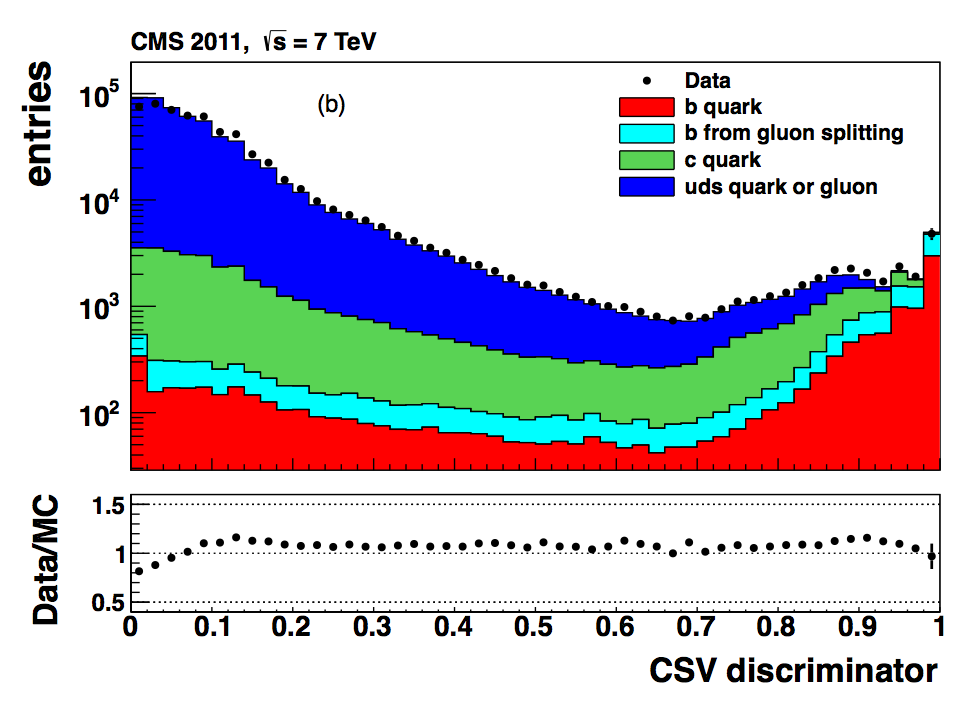
\includegraphics[width=0.7\linewidth]{Figs/CSV_discriminator_values.png}
\caption{\label{fig:csv_discriminant_values}
Plot of data and MC overlaid. The MC contains samples of jets originating from different quarks including b and light flavor~\cite{btagging}.
}
\end{center}
\end{figure}
	
	
	
	
	
	
	
	
	
	


\chapter{ttZ and Backgrounds}
		\section{specifics of ttZ production}
	\section{specifics of ttZ decay}
	After the hard collision, 3 objects exist that will be indirectly studied: a top, an anti-top, and a Z boson. For all intents and purposes, the top and anti-top particles behave similarly just swapping the matter and anti-matter labels in the decay products. A top quark is very massive at \~ 173 \GeV of energy and thus decays very quickly. There is no time for it to decay via the strong force and a hadronize, so it does not form jets. The top quark can only decay to a W boson plus a down-type quark which is a b-quark the vast majority of the time. \\
	
	The b-quarks from the top and anti-top will hadronize and form b-jets which can be reconstructed with varying degrees of efficiency and purity (see Section ~\ref{}) and act as markers for top events as high quality b-tags are fairly except in top or boson decays. The W and Z bosons will decay either to hadronic or leptonic final states. The W decays to either a lepton and a neutrino (\~ 11\% per lepton flavor ~\cite{PDG}) or to an up-type quark and a down-type quark (weakly). For the Z boson, quark anti-quark pairs are common (the most being \bbbar pairs which decay contributes to the \ttZ backgrounds) and also to lepton anti-lepton pairs (\~ 3.3\% per lepton flavor ~\cite{PDG}).\\
	
	Thus several final states exist:
	\begin{enumerate}
	\item 8 quarks (at least 2 of which are b-quarks)
	\item 6 quarks (at least 2 of which are b-quarks), 1 lepton, and 1 neutrino
	\item 6 quarks (at least 2 of which are b-quarks) and 2 leptons
	\item 4 quarks (at least 2 of which are b-quarks), 2 leptons, and 2 neutrinos
	\item 4 quarks (at least 2 of which are b-quarks), 3 leptons, and 1 neutrino
	\item 2 b-quarks, 4 leptons, and 2 neutrinos
	\end{enumerate}
	
	Thus there are several different signatures to look for in order to identify a \ttZ decay. As shown in Fig. ~\ref{fig:ttZ_decay_rates}, hadronic decays of the bosons are more common. However, the rate of decay must be balanced agains how unique and easy to distinguish (measure and reconstruct its elements in the detector) from the background processes.
	
	\begin{figure}[h]
\begin{center}

\includegraphics[width=0.48\linewidth]{Figs/placeholder.pdf}
\caption{\label{fig:ttZ_decay_rates}
Fraction of time \ttZ decays to various final states.
}
\end{center}
\end{figure} 

	
	\section{reasons for choosing 3 lepton final state}
	In order to measure the \ttZ cross section, the final state of 4 quarks (at least 2 of which are b-quarks), 3 leptons, and 1 neutrino was chosen. This system has the advantage of several distinguishing features which make up for it's lower rate of production. 2 of the leptons come from a Z decay and thus a mass constraint around the nominal Z mass of \zmass can be used to remove events with 2 leptons from events without a Z. The 3rd lepton creates a rarer final state because it is unusual for a single lepton to be produced except in W decays, and there is no decay that produces 3 leptons from one decay. All of the states benefit from the presence of b-quarks which come from the top decay because this provides a handle to help eliminate some of the dominant backgrounds like WZ production.\\
	
	The electrons provide added bonuses in that their energy and momentum can be measured with a very high precision compared to jets, so they can be used to fairly accurately reconstruct masses such as the Z mass and the W \mt. Reconstructing these masses and showing a familiar distribution helps to bolster the claim of a \ttZ discovery. 
		\section{Backgrounds}
	\label{sec:background_sources}
	A background is any type of event that will pass the signal selection yet be produced by some mechanism or particle decay that is not the desired source of the signal. Usually backgrounds are categorized by common characteristics so that they may be better estimated and subtracted from the measured number of events. For the \ttZ cross section measurement, there are 3 distinct background categorizations that will be described in the following.
	
	        		\subsection{Backgrounds From Irreducible Sources} 
	Despite all attempts to reduce the backgrounds by requiring stringent cuts on leptons, mass windows, jets, and so on, there are some processes that will just pass all of the cuts. These are known as irreducible backgrounds. For \ttZ, these backgrounds primarilly have \ttbar pairs produced in association with something else (like a boson). Table ~\ref{tab:irreducible_bkg} contains a list of irreducible backgrounds. These sources are estimated from Monte Carlo simulations in Sec~\ref{sec:irreducible_estimation}.
	\begin{table}[hbt]
	\caption{\label{tab:irreducible_bkg} Irreducible backgrounds listed in order of significance. Additional properties of the event needed to pass the selections are listed.}
	\begin{center}
	\begin{tabular}{l|ll|c}\hline\hline % L | LL | L dividers and justification
	Process & Decay Products & Other Special Features & Exp. Contribution\\
	\hline
	\ttW & 3L + 2b& 2 ISR/FSR Jets& Large\\
	\tbZ & 3L + 2b& 2 ISR/FSR Jets & Large\\
	\ttH & 3L + 2b + 2j & & Large \\
	\ttG & 3L + 2b + 2j & & Small \\
	\ttWW & 3L + 2b +2j& & Small\\
	\WZZ & 3L + 2b & 2 ISR/FSR Jets & Small\\
	\ZZZ & 3L + 2b & One lepton not identified\\ 
	         &               & \ + 2 ISR/FSR Jets & Small\\
	
	\hline \hline
	\end{tabular}
	
	\end{center}
	\end{table}
	
	
	
	
		\subsection{Non-prompt Leptons}		
		The \ttZ signature being measured requires 3 leptons to be reconstructed and identified. Specifically the leptons should be produced from near nominal mass W or Z boson decays. Further these bosons should have been produced either from a top decay or as part of the underlying collision. The source of the leptons cannot be directly measured but can be inferred from various properties with varying levels of false positives and negatives. A lepton produced from a W or Z boson decay is known as a ``real'' lepton. It is characterized primarily by moderate \pt, that on average is around half the mass of the parent boson. It also is detected alone with very small amounts of energy around it in the detector and originates from very near the primary vertex. Ones produced by other means are known as ``fake'' leptons. Fake leptons primarily are characterized by extra energy surrounding the lepton (indicative of being from a hadronic source like a b-quark) and often do not originate from near the primary vertex. A fake lepton may actually be an object that looks like a lepton in the detector (such as a pion that does not leave its energy as expected in the hadronic calorimeter). More confusingly, it may also be a true lepton that arises from a source that is not an interesting underlying event (such as a b-quark which decays to a far off mass W which then decays to a lepton and neutrino).\\
		
		The ``fake'' leptons come from sources that are not well modeled in Monte Carlo, and must be estimated by a method using data control regions. A description of the estimation method is described in Sec~\ref{sec:fake_estimation}. The primary source of fake leptons is semi-leptonic b decays. Thus events with top quarts are heavy sources of fake leptons. %See Fig~\ref{fig:tt_w_fake} for an example of \ttbar contributing to the three lepton measurement. 
The chance of an event having two fake leptons is exponentially down from a single fake lepton due to the probability of two single b-quarks decaying semi-leptonicaly and further reduced by the probability of an event containing enough b-quarks (or light flavor quarks mis-tagged as b-jets) to both produce the fake leptons and have b-tagged jets passing the selections. Thus,  events with double fakes are considered negligible. The following sections will summarize which background processes may pass selections due to a fake lepton being present.\\
		
%			\begin{figure}[h]
%\begin{center}
%
\includegraphics[width=0.48\linewidth]{Figs/placeholder.pdf}
%\caption{\label{fig:tt_w_fake}
%Example of a \ttbar event with a fake lepton to pass the three lepton requirements.
%}
%\end{center}
%\end{figure} 
	


	Table~\ref{tab:fake_bkg} lists the processes that contribute to the background events due to the inclusion of a ``fake'' lepton which does not come from a W or Z decay. These backgrounds are primarily comprised of events with \ttbar or multi-bosons in them that also have the potential to produce several jets. However, some productions with very large cross sections also contribute like the Z or W production. These events make up for the very low probability of extra jets and fake leptons through sheer commonness.
			
	\begin{table}[hbt]
	\caption{\label{tab:fake_bkg} Fake background sources are listed with additional event properties required to pass the selections.}
	\begin{center}
	\begin{tabular}{l|ll|c}\hline\hline % L | LL | L dividers and justification
	Process & Decay Products & Other Special Features & Exp. Contribution\\
	\hline
	\ttbar & 2L + 2b & 2 ISR/FSR Jets + Fake & Large\\
	ZZ & 2L + 2b & 2 ISR/FSR Jets + Fake & Small\\
	WZ & 2L + 2j & 2b + Fake & Small\\
	Z & 2L & 2 ISR/FSR Jets + 2b + Fake & Very Small\\
	WW & 2L & 2 ISR/FSR Jets + 2b + Fake & Very Small\\
	W & 1L & 2 ISR/FSR Jets + 2b + 2 Fakes & Very Small\\
	\hline \hline
	\end{tabular}
	
	\end{center}
	\end{table}



\subsection{Non-top Originating b-Jets}
Other events with the requisite number of leptons provide a false positive because of b-quarks that do not arise from top decays. There are three main sources that will provide these non-top b-quarks.
\begin{itemize}
\item Z decay to \bbbar ($\sim$15\% decay rate~\cite{pdg})
\item Light flavor (usually c-quarks) mis-tagged as b-jets
\item Gluon splitting to \bbbar
\end{itemize}

Item 1 is well modeled in Monte Carlo, but item 2 and 3 are not. Events that have b-quarks from a Z decay, tend to fail other selections or have very small cross sections and are a relatively small backgrounds. The primary source of extra b-jets is gluon splitting to \bbbar pairs (see Figure~\ref{fig:gluon_splitting}). The gluons are provided by initial state radiation as a any of the quarks present in the reaction can radiate a gluon or fuse into a gluon in higher order diagrams. These b-quarks tend to be heavily collimated, but some times have enough angular separation to be reconstructed as two distinct b-jets. These events are not well simulated in Monte Carlo and should be measured in a data control region. Additionally, as the \ttZ events exist in a jet rich environment, light flavor mistags will definitely contribute to false positives. Some attempt is made to correct for them in Monte Carlo simulation by using Data to MC scale factors that have been measured by the b-tag working group~\cite{BTV11003}. However, measuring the rate at which events pass the selection in a data control region is still the best way to estimate these backgrounds. Estimation of this type of background will be described in Sec~\ref{sec:brate_estimation}. \\

			\begin{figure}[h]
\begin{center}
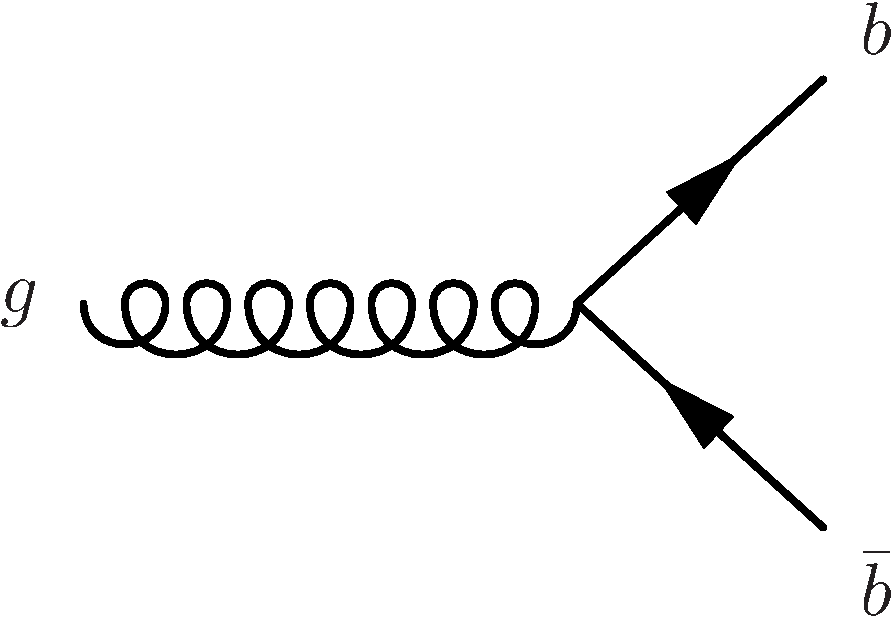
\includegraphics[width=0.48\linewidth]{Figs/gluon_splitting.pdf}
\caption{\label{fig:gluon_splitting}
Diagram of gluon splitting where the b-quarks are from not top events. The gluon can radiate from any hadronic source.
}
\end{center}
\end{figure} 


		Table~\ref{tab:bjet_bkg} lists the processes that contribute background events due to b-jets being measured either due to a b-quark that does not originate from a top or due to a b-jet that is a mis-tagged light flavor jet. These sources primarily are multi-boson samples that have the leptons to pass the selection but do not normally produce b-quarks.

	\begin{table}[hbt]
	\caption{\label{tab:bjet_bkg} Backgrounds which contain non-top originating b-jets are listed with additional required properties to pass event selections.}
	\begin{center}
	\begin{tabular}{l|ll|c}\hline\hline % L | LL | L dividers and justification
	Process & Decay Products & Other Special Features & Exp. Contribution\\
	\hline
	WZ & 3L & 2b  & Large\\
	ZZ & 4L & 2 ISR/FSR Jets + 2b + lost lepton & Medium\\
	WWW & 3L & 2 ISR/FSR Jets + 2b& Small\\
	WWZ & 3L + 2j & 2 b & Small\\
	\hline \hline
	\end{tabular}
	
	\end{center}
	\end{table}



		

			  
		
			
			
			
			
			


\chapter{Samples}
\label{ch:samples}
\section{Collision Data Samples}
	
	
Signal events are selected from the datasets and run ranges listed in Table~\ref{tab:DilDsets}.  The fake rate measurement is performed using those listed in Table~\ref{tab:FRDsets}.  Runs found in the Run2012A 06Aug2012 recover are excluded from the Run2012A 13Jul2012 re-reco dataset. 

\begin{table}[hbt]
\begin{center}
\begin{tabular}{lcc}\hline\hline
Name		& Run Range & Luminosity ($fb^{-1}$) \\ \hline
\verb=/DoubleMu/Run2012A-recover-06Aug2012-v1/AOD=                 & 190782 - 190949 &  0.081 \\ 
\verb=/DoubleMu/Run2012A-13Jul2012-v1/AOD=                                  &  190456 - 193621       & 0.796               \\ 
\verb=/DoubleMu/Run2012B-13Jul2012-v4/AOD=                                  &  193834 - 196531        & 4.412             \\ 
\verb=/DoubleMu/Run2012C-24Aug2012-v1/AOD=                                &  197770 - 198913  & 0.473\\  
\verb=/DoubleMu/Run2012C-PromptReco-v2/AOD=                               &  198934 - 203755     & 6.330                \\ 
\verb=/SingleMu/Run2012C-EcalRecover_11Dec2012-v1/AOD=          & 201 191 - 201 191 & 0.133\\
\verb=/DoubleMu/Run2012D-PromptReco-v1/AOD=                               &  203768 - 208913  &  7.295 \\
%\verb=/DoubleMu/Run2012D-16Jan2013-v1/AOD=                                 &  207883 - 208307  \\

\verb=/DoubleElectron/Run2012A-recover-06Aug2012-v1/AOD=         &    190782 - 190949     & 0.081              \\ 
\verb=/DoubleElectron/Run2012A-13Jul2012-v1/AOD=                         & 190456 - 193621   & 0.796                    \\ 
\verb=/DoubleElectron/Run2012B-13Jul2012-v1/AOD=                         &  193834 - 196531  & 4.412\\ 
\verb=/DoubleElectron/Run2012C-24Aug2012-v1/AOD=                       &  197770 - 198913    & 0.473                 \\ 
\verb=/DoubleElectron/Run2012C-PromptReco-v2/AOD=                     &   198934 - 203755     & 6.330             \\ 
\verb=/SingleMu/Run2012C-EcalRecover_11Dec2012-v1/AOD=          & 201 191 - 201 191 & 0.133\\
\verb=/DoubleElectron/Run2012D-PromptReco-v1/AOD=                      &  203768 - 208913  &  7.295 \\
%\verb=/DoubleElectron/Run2012D-16Jan2013-v2/AOD=                        &   207883 - 208307 \\

\verb=/MuEG/Run2012A-recover-06Aug2012-v1/AOD=                          &      190782 - 190949     & 0.081            \\ 
\verb=/MuEG/Run2012A-13Jul2012-v1/AOD=                                          &  190456 -193621         & 0.796             \\ 
\verb=/MuEG/Run2012B-13Jul2012-v1/AOD=                                         &  193834 -196531      & 4.412 \\ 
\verb=/MuEG/Run2012C-24Aug2012-v1/AOD=                                      &   197770 - 198913     & 0.473               \\ 
\verb=/MuEG/Run2012C-PromptReco-v2/AOD=                                     &   198934 - 203755      & 6.330              \\ 
\verb=/SingleMu/Run2012C-EcalRecover_11Dec2012-v1/AOD=          & 201 191 - 201 191 & 0.133\\
\verb=/MuEG/Run2012D-PromptReco-v1/AOD=                                     &  203768 - 208913  &  7.295 \\
%\verb=/MuEG/Run2012D-16Jan2013-v2/AOD=                                       &  203768 - 208307 \\

\verb=/SingleMu/Run2012A-recover-06Aug2012-v1/AOD=                    &   190782 - 190949          & 0.081          \\ 
\verb=/SingleMu/Run2012A-13Jul2012-v1/AOD=                                     &  190456 - 193621      & 0.796                \\ 
\verb=/SingleMu/Run2012B-13Jul2012-v1/AOD=                                     &  193834 - 196531  & 4.412 \\ 
\verb=/SingleMu/Run2012C-24Aug2012-v1/AOD=                                   &   198022 - 198523     & 0.473               \\ 
\verb=/SingleMu/Run2012C-PromptReco-v2/AOD=                                  &   198934 - 203755    & 6.330                \\ 
\verb=/SingleMu/Run2012C-EcalRecover_11Dec2012-v1/AOD=          & 201 191 - 201 191 & 0.133 \\
\verb=/SingleMu/Run2012D-PromptReco-v1/AOD=                                  &  203768 - 208913   &  7.295 \\



 \hline\hline
\end{tabular}
\caption{\label{tab:DilDsets}Datasets used to select signal events.}
\end{center}
\end{table}

\begin{table}[hbt]
\begin{center}
\begin{tabular}{lc}\hline\hline
Name		& Run Range \\ \hline
\verb=/DoubleMu/Run2012A-recover-06Aug2012-v1/AOD=                 &   190782 - 190949\\ 
\verb=/DoubleMu/Run2012A-13Jul2012-v1/AOD=                                  &  190456 - 193621                     \\ 
\verb=/DoubleMu/Run2012B-13Jul2012-v4/AOD=                                  &  193834 - 196531                     \\ 
\verb=/DoubleMu/Run2012C-24Aug2012-v1/AOD=                                &  197770 - 198913 \\  
\verb=/DoubleMu/Run2012C-PromptReco-v2/AOD=                               &  198934 - 203755                     \\ 
\verb=/DoubleMu/Run2012D-PromptReco-v1/AOD=                               &  203768 - 208913  \\
\verb=/DoubleMu/Run2012D-16Jan2013-v1/AOD=                                 &  207883 - 208307  \\

\verb=/DoubleElectron/Run2012A-recover-06Aug2012-v1/AOD=         &   190782 - 190949                    \\ 
\verb=/DoubleElectron/Run2012A-13Jul2012-v1/AOD=                         & 190456 - 193621                      \\ 
\verb=/DoubleElectron/Run2012B-13Jul2012-v1/AOD=                         &  193834 - 196531 \\ 
\verb=/DoubleElectron/Run2012C-24Aug2012-v1/AOD=                       &   197770 - 198913                    \\ 
\verb=/DoubleElectron/Run2012C-PromptReco-v2/AOD=                     &    198934 - 203755                  \\ 
\verb=/DoubleElectron/Run2012D-PromptReco-v1/AOD=                      &  203768 - 208913  \\
\verb=/DoubleElectron/Run2012D-16Jan2013-v2/AOD=                        &   207883 - 208307 \\

\verb=/SingleMu/Run2012A-recover-06Aug2012-v1/AOD=                    &     190782 - 190949                  \\ 
\verb=/SingleMu/Run2012A-13Jul2012-v1/AOD=                                     &  190456 - 193621                     \\ 
\verb=/SingleMu/Run2012B-13Jul2012-v1/AOD=                                     &  193834 - 196531 \\ 
\verb=/SingleMu/Run2012C-24Aug2012-v1/AOD=                                   &   198022 - 198523                   \\ 
\verb=/SingleMu/Run2012C-PromptReco-v2/AOD=                                  &   198934 - 203755                    \\ 
\verb=/SingleMu/Run2012D-PromptReco-v1/AOD=                                  &  203768 - 208913   \\
 \hline\hline
\end{tabular}
\caption{\label{tab:FRDsets}Datasets used to measure the lepton fake rates.}
\end{center}
\end{table}

\subsection{Data Certification}
\label{sec:data_details:cert}

Only certified data from the datasets and run ranges listed in Appendix~\ref{sec:data_details:datasets} is included in the analysis.  The list of good data taking periods is taken from a combination of the following prompt and re-reco certifications:


\clearpage	
	
	
	
	
\section{Monte Carlo Simulation Samples}
\label{sec:MCSamples}


Table~\ref{tab:IrreducibleMCSamples} contains a list of Monte Carlo samples contributing to the SM background from rare processes that is taken from simulation.  The cross section and equivalent luminosity of each sample is also provided. \ttZ \ is included in this table as it is used in the spillage subtraction in the fake rate.

\begin{sidewaystable}[H]
\begin{center}
\begin{tabular}{lcc}
\hline\hline
Name														           & Cross section, pb & Luminosity, \fbinv \\ \hline
\verb=/TTZJets_8TeV-madgraph/Su12-v1=                                                                 & 0.206                     &       1021.68         \\ 
\verb=/TTWWJets_8TeV-madgraph/Su12 V7A=                                                            & 0.002037          &      106932       \\ 
\verb=/TTWJets_8TeV-madgraph/Su12 V7A=                                                               & 0.232             &        845.026         \\ 
\verb=/TTGJets_8TeV-madgraph/Su12 V19=                                                                & 2.166             &       775.602          \\ 
\verb=/TBZToLL_4F_TuneZ2star_8TeV-madgraph-tauola/Su 12 V7C=                 &  0.0114             &         13026.7        \\
\verb=/WZZNoGstarJets_8TeV-madgraph/Su12 V7A=                                               & 0.01922           &       12946.7        \\ 
\verb=/ZZZNoGstarJets_8TeV-madgraph/Su12 V7A=                                                 & 0.004587          &     40692.6          \\ 
\hline\hline
\end{tabular}
\caption{\label{tab:IrreducibleMCSamples} MC datasets corresponding to contributions not covered by the data-driven methods.
Predicted yields from the SM samples listed here are used directly in the analysis. 
The common part of each dataset name {\tt Summer12\_DR53X-PU\_S10\_START53\_V7X-v1} is replaced with a shorthand {\tt Su12 V7X}. 
All datasets are in the AODSIM data tier.}
\end{center}
\end{sidewaystable}

\clearpage

\begin{sidewaystable}[H]
\begin{center}
\begin{tabular}{lcc}
\hline\hline
Name                                                                                                                             & Cross section, pb & Luminosity, \fbinv \\ \hline
\verb=/TTJets_SemiLeptMGDecays_8TeV-madgraph-tauola/Su 12 V7C-v1= & 102.50 & 247.657\\
\verb=/TTJets_FullLeptMGDecays_8TeV-madgraph/S 12V7A-v2=                    &  24.56       & 493.445\\
\verb=/DY1JetsToLL_M-50_TuneZ2Star_8TeV-madgraph/Su 12 V7A=           &   671.83          &       35.4483 \\
\verb=/DY2JetsToLL_M-50_TuneZ2Star_8TeV-madgraph/Su 12 V7C=           &  216.76            &    100.444    \\
\verb=/DY3JetsToLL_M-50_TuneZ2Star_8TeV-madgraph/Su 12 V7A=           &   61.2          &      178.847  \\
\verb=/DY4JetsToLL_M-50_TuneZ2Star_8TeV-madgraph/Su 12 V7A=           &  27.59           &   232.071     \\ 
\verb=/W1JetsToLNu_TuneZ2Star_8TeV-madgraph/Su 12 V7A=                     &    6663                    &  3.47315 \\
\verb=/W2JetsToLNu_TuneZ2Star_8TeV-madgraph/Su 12 V7A=                     &    2159                    &  15.7688 \\
\verb=/W3JetsToLNu_TuneZ2Star_8TeV-madgraph/Su 12 V7A=                     &   640                    &  24.2805 \\
\verb=/W4JetsToLNu_TuneZ2Star_8TeV-madgraph/Su 12 V7A=                     &    264                    & 50.6924 \\
\verb=/WWJetsTo2L2Nu_TuneZ2star_8TeV-madgraph-tauola/Su 12 V7A=      &  5.8123            &     332.611             \\ 
\verb=/WZJetsTo2L2Q_TuneZ2star_8TeV-madgraph-tauola/Su 12 V7A=      &    2.206            &        1457.84          \\
\verb=/ZZJetsTo2L2Q_TuneZ2star_8TeV-madgraph-tauola/Su 12 V7A=      &     2.4487          &        790.921          \\
\hline\hline
\end{tabular}
\caption{\label{tab:frEstimatedMCSamples} MC datasets that do not contribute to MC Pred.  The contribution to the background from these processes is covered by data-driven methods, but expected yields based on simulation are nevertheless provided as a reference.
Predicted yields from the SM samples listed here are used directly in the analysis. 
The common part of each dataset name {\tt Summer12\_DR53X-PU\_S10\_START53\_V7A} is replaced with a shorthand {\tt Su12 V7A}. 
All datasets are in the AODSIM data tier.}
\end{center}
\end{sidewaystable}

\clearpage


\begin{sidewaystable}[H]
\begin{center}
\begin{tabular}{l}
\hline\hline
Name                                                                                                                              \\ \hline
\verb=/QCD_Pt_20_MuEnrichedPt_15_TuneZ2star_8TeV_pythia6/Su 12 V7A-v3=                       \\
\verb=/QCD_Pt-15to20_MuEnrichedPt5_TuneZ2star_8TeV_pythia6/Su 12 V7A-v2=                       \\
\verb=/QCD_Pt-20to30_MuEnrichedPt5_TuneZ2star_8TeV_pythia6/Su 12 V7A-v1=                        \\
\verb=/QCD_Pt-30to50_MuEnrichedPt5_TuneZ2star_8TeV_pythia6/Su 12 V7A-v1=                        \\
\verb=/QCD_Pt-50to80_MuEnrichedPt5_TuneZ2star_8TeV_pythia6/Su 12 V7A-v1=                     \\
\verb=/QCD_Pt-80to120_MuEnrichedPt5_TuneZ2star_8TeV_pythia6/Su 12 V7A-v1=                       \\
\verb=/QCD_Pt-120to170_MuEnrichedPt5_TuneZ2star_8TeV_pythia6/Su 12 V7A-v1=                       \\
\verb=/QCD_Pt-5to15_TuneZ2star_8TeV_pythia6/Su 12 V7A-v1=                        \\
\verb=/QCD_Pt-15to30_TuneZ2star_8TeV_pythia6/Su 12 V7A-v2=                      \\
\verb=/QCD_Pt-30to50_TuneZ2star_8TeV_pythia6/Su 12 V7A-v2=                      \\
\verb=/QCD_Pt-50to80_TuneZ2star_8TeV_pythia6/Su 12 V7A-v2=                        \\
\verb=/QCD_Pt-80to120_TuneZ2star_8TeV_pythia6/Su 12 V7A-v3=                     \\
\verb=/QCD_Pt-120to170_TuneZ2star_8TeV_pythia6/Su 12 V7A-v3=                       \\
\verb=/QCD_Pt-170to300_TuneZ2star_8TeV_pythia6/Su 12 V7A-v2=                        \\
\hline\hline
\end{tabular}
\caption{\label{tab:frQCDMCSamples} MC datasets that are used in calculated the Fake Rate used in the closure tests for the purpose of determining the systematic uncertainty on the method as well as correcting the central value of the prediction. 
The common part of each dataset name {\tt Summer12\_DR53X-PU\_S10\_START53\_V7A} is replaced with a shorthand {\tt Su12 V7A}. 
All datasets are in the AODSIM data tier.}
\end{center}
\end{sidewaystable}
\clearpage




Table ~\ref{tab:bEstimatedMCSamples} contains a list of Monte Carlo samples that are used for reference for the theoretical contributions of the processes estimated from the method that predicts he contribution of events that have b-tags from radiation.
\begin{sidewaystable}[H]
\begin{center}
\begin{tabular}{lcc}
\hline\hline
Name                                                                                                                             & Cross section, pb & Luminosity, \fbinv \\ \hline
\verb=/WZJetsTo3LNu_TuneZ2_8TeV-madgraph-tauola/Su 12 V7A=      &       1.0575        &        1908.25        \\
\verb=/ZZJetsTo4L_TuneZ2star_8TeV-madgraph-tauola/Su 12 V7A=      &         0.176908      &         27177.4         \\
\verb=/WWGJets_8TeV-madgraph/Su12 V7A=                                                            & 0.528             &        407.426         \\ 
\verb=/WWWJets_8TeV-madgraph/Su12 V7A=                                                            & 0.08217           &     2737.02           \\ 
\verb=/WWZNoGstarJets_8TeV-madgraph/Su12 V7A=                                              & 0.0633            &        3832.94        \\ 
\hline\hline
\end{tabular}
\caption{\label{tab:bEstimatedMCSamples} MC datasets that do not contribute to MC Pred.  The contribution to the background from these processes is covered by data-driven methods (b-tag estimation from radian jets), but expected yields based on simulation are nevertheless provided as a reference.
Predicted yields from the SM samples listed here are used directly in the analysis. 
The common part of each dataset name {\tt Summer12\_DR53X-PU\_S10\_START53\_V7A} is replaced with a shorthand {\tt Su12 V7A}. 
All datasets are in the AODSIM data tier.}
\end{center}
\end{sidewaystable}

\clearpage


\begin{sidewaystable}[H]
\begin{center}
\begin{tabular}{lcc}
\hline\hline
Name                                                                                                                             & Cross section, pb & Luminosity, \fbinv \\ \hline
\verb=/DYJetsToLL_M-50_TuneZ2Star_8TeV-madgraph-tarball/Su12-v1=    &        3532.8149     &         8.62188         \\ 
\verb=/WZJetsTo3LNu_TuneZ2_8TeV-madgraph-tauola/Su 12 V7A=      &        1.0575       &              1908.25    \\
\hline\hline
\end{tabular}
\caption{\label{tab:bRateComparison} MC datasets used to validate the b-tag content in a di-lepton and tril-lepton sample against each other as a demonstration of the validity of the method used to predict contribution to the background via b-tags that come from radiation. Note that the DY sample differs from that used in the rest of the analysis. This one was specifically chosen because it treats the b-quark's mass the same as in the used WZ sample.
The common part of each dataset name {\tt Summer12\_DR53X-PU\_S10\_START53\_V7A} is replaced with a shorthand {\tt Su12 V7A}. 
All datasets are in the AODSIM data tier.}
\end{center}
\end{sidewaystable}


\begin{sidewaystable}[H]
\begin{center}
\begin{tabular}{lcc}
\hline\hline
Name                                                                                                                             & Cross section, pb & Luminosity, \fbinv \\ \hline
\verb=/TTZJets_8TeV-madgraph_v2/Su 12 V7A=                                         &        0.2057     &        1021.68          \\ 
\verb=/ttbarZ_8TeV-Madspin_aMCatNLO-herwig/Su 12 V19=                    &        0.2057       &                  \\
\hline\hline
\end{tabular}
\caption{\label{tab:ttZGeneratorMCs} MC datasets used to determine the signal systematic uncertainty due to the type of generator used. They are both normalized to the same cross section. Madgraph is an LO generator while aMC@NLO is an NLO generator. The madgraph sample is the same as the one listed in table~\ref{tab:IrreducibleMCSamples}.
The common part of each dataset name {\tt Summer12\_DR53X-PU\_S10\_START53\_V7A} is replaced with a shorthand {\tt Su12 V7A}. 
All datasets are in the AODSIM data tier.}
\end{center}
\end{sidewaystable}

\clearpage

	
\chapter{Event Selections}
\label{ch::EventSelections}
Some intro here...

\section{Triggers for Data Acquisition}
\label{sec:Triggers}
As the desired final state contains 3 isolated leptons (electrons or muons), a set of triggers without pre-scaling may be used that has 1, 2, or 3 isolated leptons as the trigger requirements. The ideal trigger would have moderate \pt thresholds and would not have restrictions on $\eta$ so that leptons from anywhere in the tracker may be counted. Isolation requirements are allowed provided they are not tighter than the offline requirements of XXXXX (see Section~\ref{}). Further a parallel set of single lepton triggers must exist in order to select data measure the ratio used in the background subtraction method which estimates non-prompt lepton contamination (i.e. Fake Rate) in the signal (see Section~\ref{}). \\
Thus a variety of triggers were chosen that require 2 or more leptons (double lepton triggers). Triggers that require 1 or more lepton or that require 3 or more leptons were rejected as they would not match the triggers used to estimate the Fake Rate. The double lepton triggers are assumed to be 100\% efficient. The efficiency to trigger on 1 lepton is very high, and thus with 3 leptons, the odds that at least 2 of them will pass is approximately 100\%. A small systematic uncertainty is added to account for any potential inefficiency (see Section~\ref{}).
	
\begin{table}[h]
\begin{center}
\caption{\small\label{tab:AnalysisTriggers} Triggers used while measuring the yields in data for the main analysis selections. In the trigger name the ``v" at the end of the line stands for a number of versions that changes while data is being collected.}
\begin{tabular}{l|l} \hline \hline
Lepton Type & Trigger  \\ \hline
$\mu\mu$     & \verb=HLT_Mu17_Mu8_v= \\
$\mu \mu$    &\verb=HLT_Mu17_TkMu8_v= \\
ee                   & \verb=HLT_Ele17_CaloIdT_CaloIsoVL_TrkIdVL_TrkIsoVL_v= \\
ee                   & \verb=Ele8_CaloIdT_CaloIsoVL_TrkIdVL_TrkIsoVL_v=\\
$\mu$e          & \verb=HLT_Mu17_Ele8_CaloIdT_CaloIsoVL_TrkIdVL_TrkIsoVL_v= \\
$\mu$e          & \verb=HLT_Mu8_Ele17_CaloIdT_CaloIsoVL_TrkIdVL_TrkIsoVL_v= \\
\hline
\end{tabular}
\end{center}
\end{table}

Events are required to fire a trigger in Data only. Monte Carlo events are not required to fire a trigger. Monte Carlo triggers are not well enough simulated to accurately predict the behavior of Data triggers. This is not a problem as the Data triggers used are un-prescaled and highly efficient.




\section{General Event Cleanup and Vertex Selection}
\label{sec::EventCleanup}

Events in data and simulation are required to pass the following:

\begin{itemize}
\item Scraping cut: if there are $\geq$ 10 tracks, require at least 25\% of them to be high purity. 
\item Require at least one good primary vertex (PV), and use the first such vertex found as a reference point for further selections.  A good vertex is selected by requiring:
	\begin{itemize}
	\item not fake, ?????????
	\item ndof $>$ 4,
	\item $|\rho| < 2$ cm,
	\item $|z| < 24$ cm.  
	\end{itemize}
\end{itemize}
	 
	 
\section{High Level Event Identification}	 
\label{sec:EventSelections}
Good, isolated electrons are selected following the ``medium" identification requirements recommended by the Egamma POG~\cite{eleICHEP2012twiki}.
Electrons are required to have no missing expected inner hits~\cite{conv} and to not be reconstructed as part of a good conversion vertex~\cite{hwwsmurf} so as to suppress background from converted photons.
Additionally, electrons are required to have $\Delta R >0.1$ with respect to any muon passing the selections above.
We reject electrons found in the transition region.
The isolation follows the POG recommendation~\cite{egammapfisotwiki}, using particle-flow based isolation with a cone size of \DR\  $=$ 0.3.  
Subtraction for PU is performed by removing a term defined by the product of the average event energy density and the effective area of the isolation cone from the neutral isolation sum~\cite{egammaisorhoaeff}.
The isolation relative to the electron \pt\ is required to be less than 0.09.\\

Event selections were designed to be middle ground - a compromise between strong background rejection and inclusiveness. It is done in 5 main steps:
\begin{enumerate}
\item Identify a Z candidate consisting of two isolated high \pt \ leptons (20 \GeV ) with opposite electric charge and of the same flavor that are within a $\pm 10$ \GeV window of the Z invariant mass (\zmass);
\item Identify a third lepton which could be the result of a W decay passing the same identification and isolation requirements as the Z leptons;
\item Reject events with a 4th lepton passing a looser set of selections (identification loosened to the standard EGamma medium working point and Muon tight working point and $\pt > 10 \ \GeV$) to be exclusive with the 4 Lepton channel;
\item Identify at least 4 Jets to be consistent with the number from a semi-leptonic $t\bar{t}$ decay;
\item Identify from the Jets at least 2 that pass the CSV b-Tagging algorithm;
\end{enumerate}	 
	 
\section{electron selections}
\label{sec:ElectronSelections}

Electron candidates are RECO GSF electrons with \pt\ \gt\ 20 \GeV\ and \absetaele\ passing the following requirements recommended by the Egamma POG~\cite{eleICHEP2012twiki}:
\begin{itemize}
\item reject electrons in the transition region $1.4442 < \aeta < 1.556$, where $\eta$ is taken from the super-cluster (SC);
\item electrons have to have $\DR >0.1$ with respect to any muon passing the selections in Appendix~\ref{sec:muID};
\item cut-based medium WP as defined by~\cite{eleICHEP2012twiki};
\item transverse impact parameter of the GSF track with respect to the selected PV to be $<200~\micron$;
\item the $z$ coordinate of the GSF track should be within 2~mm with respect to that of the selected PV;
\item Conversion removal by veto of a good reconstructed conversion vertex.  A conversion vertex is considered good if it has no tracker hits towards the beam, has a fit probability above $10^{-6}$, has a displacement of more than 2~cm, and the  CTF track matching to the electron should be a part of the conversion vertex. No requirement is made on the vertex quality flag corresponding to merging and arbitration~\cite{hwwsmurf}.
\end{itemize}

Additionally, the identification contains the following modifications/additions with respect to the above recommendation:

\begin{itemize}
\item the number of missing expected inner hits must be zero~\cite{conv};

\item the $H/E$ is required to be \lt 0.1 (0.075) in the barrel (endcap) to match the requirements in the trigger.
\end{itemize}

The isolation follows the POG recommendation, using particle-flow based isolation with a cone size of \DR  $=$ 0.3~\cite{egammapfisotwiki}.  
In the endcap, an inner veto of \DR $=$ 0.015 (0.08) is imposed for charged hadrons (photons). 
The isolation is corrected for PU by subtracting from the neutral isolation components a term defined by the product of the average event energy density and the effective area of the isolation cone~\cite{egammaisorhoaeff}.  The neutral component after correction is required to be non-negative.  
The isolation relative to the electron \pt\ is required to be less than 0.09.



\section{muon selections}
\label{sec:MuonSelections}
Muons are required to be well identified and isolated, passing the ``tight" identification requirements recommended by the muon POG~\cite{muICHEP2012twiki}. Additionally veto deposits are required to be consistent with a minimum ionizing particle and the d0 requirement is tightened to reduce non-promt lepton contamination.  
Isolation follows the POG recommendation, using  particle-flow based isolation with a $\Delta\beta$ correction for PU and a threshold of 0.1.
A smaller cone size of \DR\ $=$ 0.3 is adopted due to the high hadronic activity expected in signal-like events.\\

Muon candidates are RECO muon objects with \pt\ \gt\ 20 \GeV\ and \absetamu\ and passing the ``tight" identification requirements recommended by the muon POG~\cite{muICHEP2012twiki}:
\begin{itemize}
\item is a global muon;
\item is a particle flow muon;
\item $\chi^2$/ndof of global fit $<$ 10;
\item at least 6 layers with hits in the tracker;
\item the global fit has to include at least one valid hit in the muon subdetectors;
\item there are muon segments in at least two muon stations. Note, this implies that the muon is also an arbitrated tracker muon~\cite{swguidetrackermuonstwiki};
\item at least one pixel hit.
\end{itemize}

Additionally, the identification contains the following modifications/additions with respect to the above recommendation:

\begin{itemize}
\item transverse impact parameter of the silicon (inner) track with respect to the selected PV to be $<200~\micron$;
\item the inner track $z$ should be within 1~mm from the selected PV;
\item ECAL veto deposit \lt\ 4~\GeV\ (veto deposit corresponds to the sum of $E_T$ in the region of the calorimeter
associated with the muon impact);
\item HCAL veto deposit \lt\ 6~\GeV.
\end{itemize}

The isolation follows the POG recommendation, using particle-flow based isolation with a $\Delta\beta$ correction for PU.  
However, a smaller cone size of \DR\ $=$ 0.3 is adopted due to the high hadronic activity expected in signal-like events.  
The isolation calculated using 
$$
\relIso = [ \Sigma_{\rm ch} + {\rm max}(0, \Sigma_{\rm nh} + \Sigma_{\rm ph} - 0.5 \Delta\beta) ]/\pt,
$$
where $\Sigma_{\rm ch, nh, ph}$ are the sums of \pt\ of the charged hadron, neutral hadron, and photon particle flow candidates, respectively.
Here the charged hadrons are matched to the PV and a 0.5~\GeV\ threshold is applied on neutral hadrons and photons.  
The $\Delta\beta$ correction is det	``ermined from the sum \pt\ of charged hadrons not matched to the PV with a threshold of 0.5~\GeV\ in a cone of the same size as the isolation.  
 
The \relIso\ is required to be less than 0.1.


\section{Z-boson lepton pair and 3rd lepton selection}
\label{sec:3LepSelection}
All 3 selected leptons must pass the Identification and Isolation requirements as well as \pt and $\eta$ requirements listed in Sections \ref{} and \ref{}. Furthermore, 2 of the leptons are required to be consistent with a reconstructed Z boson. This includes:
\begin{itemize}
\item opposite charge
\item same flavor
\item invariant mass between 81 and 101 GeV
\item both leptons matched to the same vertex
\end{itemize}
In the case of events where all three leptons are the same flavor and two combinations exist which fit in the invariant mass window, the one which is closest to the measured Z mass of \zmass \ ~\cite{pdg} is chosen.\\

\section{4th lepton veto}
\label{sec:4thLeptonVeto}
To be accepted as an event, three tight leptons as described in Appendix ~\ref{sec:muID} and ~\ref{sec:eleID} must be found. A veto on a fourth lepton passing the unmodified POG recommendations used as the base cuts above is applied. In addition, the 4th lepton has a relaxed \pt \ requirement of 10 \GeV. Finally, the same isolation requirements as above are used.

\section{jet selection}
\label{sec:JetSelection}
There must be at least 3 particle-flow jets with $\pt > 30$ GeV and $|\eta| < 2.5$ and at least a fourth particle-flow jet with $\pt > 15$ GeV and $|\eta| < 2.5$. The threshold on the fourth jet is lowered as this one tends to be produced softer than the other jets.
Jets are reconstructed with the anti-$k_{T}$ algorithm with parameter R = 0.5.  
Jets in simulation have L1FastJetL2L3 (FastJet-based offset correction followed by L2 and L3 corrections) corrections applied.  
Jets in data additionally have L2L3 residual corrections applied~\cite{jetcorrectionstwiki}. 
Selected jets must pass loose {\tt pfJetId} and be separated by $\Delta R >$ 0.5 from any lepton passing the selections above. Finally, an extra pile up rejection is applied where at least 10\% \ of the energy in the jet must be from within a $dZ < 0.05 cm$ of the primary vertex.

\section{b-tag selection}
\label{sec:bTagSelection}

Include details about tagger efficiency and purity as well as some basic info about how it works???????????\\

At least two jets passing the above jet selections in \ref{} and $\pt > 30$ are required to be tagged using the CSV algorithm. Both must be at least passing the loose threshold, and one must be at least passing the medium threshold.
This tagger identifies jets with discriminant larger than  0.244 as Loose b-tagged and 0.679 as Medium b-tagged~\cite{btagICHEP2012twiki}.




\section{optimization}
\label{sec:Optimization}

While defining the event selections, a number of options were considered. All of the selections were chosen to simultaneously reduce the  background compared to signal and the projected error on the cross section using the \ttZ \ signal Monte Carlo and full analysis background estimates. This includes \Ht \ cuts, \met \ cuts, alternative thresholds and multiplicities for b-tagging, alternative  \pt cuts and multiplicities for jets, and varying sized Z mass windows. In the end, too many backgrounds have real \met \ from a $W \rightarrow \ell \nu$ decay for this to be a distinguishing variable. Although \Ht \ can be used to reduce many of the backgrounds, it ended up performing not quite as well as and being redundant with the (related) pure jet cuts used in this note. Additionally, a single tight or medium  b-tag was found to let in too much background, while using 2 mediums or a medium and a tight killed too much signal.  

Optimizing the Z mass window ends up being less straightforward than the other relevant selections. The Z mass window makes little difference in the error on the cross section and was thus chosen by its expected signficance (Table ~\ref{tab:zmass_errorsig}). In Table~\ref{tab:zmass_errorsig}, the significance continues to increase with an even narrower Z mass window than the chosen $\pm 10$ \GeV \ window, but there is a strong reason to stop at $\pm 10$ \GeV.\\

These predictions are made with the assumption that no new systematic uncertanties are introduced. This assumption does not hold up for a narrow enough Z mass window. By comparing the yields of the \ttZ \ signal MC to a 2 lepton Z selection in data, the yields do not scale the same. The 2 lepton Z selection is the same as used to calculate the rate of b-tagged jets in the background estimate of non-top process. Table ~\ref{tab:zmass_massscaling} shows the \ttZ scaling and the 2 lepton data scaling both with a b-veto applied as well as a 2 b-tag selection applied. The reference yields are from the $\pm 15$ \GeV \ Z mass window. The 2 lepton Z data selection is chosen because it is high in statistics and not part of our signal region (yet contains a reconstructed Z boson).

As the window gets narrower beyond $\pm 10$ \GeV, the difference in scaling of the yields in Table ~\ref{tab:zmass_massscaling} becomes significant at approximately a difference of 4-5\%. These narrower mass windows would lead to challenges in estimating the systematic uncertainty introduced by the mass window as well as reduce the significance of that mass window. To avoid this extra difficulty, the $\pm 10$ \GeV \ window is chosen.

\begin{table}[ht!]
\caption{\small \label{tab:zmass_errorsig} Expected signficance and estimated \% error on the cross section by varying the Z mass window. Significance and error estimates are determined with full analysis selections and background estimates in conjunction with the \ttZ \ signal Monte Carlo.}
\begin{center}
\begin{tabular}{c|ccc}\hline
Mass Window (\GeV)   &  Expected Significance  & \multicolumn{2}{c}{Estimated Error on Cross Section}    \\
                     &                         & +         & -                                           \\
\hline \hline
$\pm 15$             &  2.27                   &  +51\%    &  -45\%                                      \\
$\pm 12.5$           &  2.42                   &  +50\%    &  -43\%                                      \\
$\pm 10$             &  2.44                   &  +50\%    &  -43\%                                      \\
$\pm 7.5$            &  2.57                   &  +49\%    &  -42\%                                      \\
$\pm 5$              &  2.51                   &  +51\%    &  -43\%                                      \\
$\pm 2.5$            &  2.21                   &  +60\%    &  -49\%                                      \\
\hline
\end{tabular}
\end{center}
\end{table}


%% \begin{table}[ht!]
%% \caption{\small \label{tab:zmass_expsig} Expected significance by varying the Z mass window. Expected significance is determined with full analysis selections and background estimates in conjunction with the \ttZ \ signal Monte Carlo.}
%% \begin{center}
%% \begin{tabular}{c|c}\hline
%% Mass Window (\GeV)  & Expected Significance            \\
%% \hline \hline
%% $\pm 15$            &  2.27 \\
%% $\pm 12.5$          &  2.42 \\
%% $\pm 10$            &  2.44 \\
%% $\pm 7.5$           &  2.57 \\
%% $\pm 5$             &  2.51 \\
%% $\pm 2.5$           &  2.21 \\

%% \hline
%% \end{tabular}
%% \end{center}
%% \end{table}


\begin{sidewaystable}[ht!]
\caption{\small \label{tab:zmass_massscaling} Scaling of yields in high statistics Z selection with Z mass window. The ``2 Lepton Data'' columns are important numbers in the calculation of the rate of b-tags and are used here because they are a high statistics selection of a Z boson. Statistical errors on the absolute yields in the \ttZ MC \ are between 5 and 6\%. Statistical errors on the DY MC are negligable while statistical errors on the 2 Lepton Data selection are between 0.5\% and 2\% where the DY MC with b-veto is clustered at the low end.}
\begin{center}
\begin{tabular}{c|ccccc}\hline
Mass Window (\GeV)  & \ttZ \ MC   & 2 Lepton DY MC  & 2 Lepton Data  & 2 Lepton DY MC  & 2 Lepton Data  \\
                    &             & with b-Veto     & with b-Veto    & with 2 b-tags   & with 2 b-tags \\
\hline \hline
$\pm 15$            &  100\%      &  100\%          & 100\%          & 100\%           & 100\%  \\
$\pm 12.5$          &  99.5\%     &  98.6\%         & 98.1\%         & 99.0\%          & 98.1\% \\
$\pm 10$            &  97.8\%     &  96.0\%         & 95.6\%         & 97.1\%          & 95.4\% \\
$\pm 7.5$           &  95.2\%     &  91.9\%         & 90.8\%         & 91.9\%          & 91.4\% \\
$\pm 5$             &  87.9\%     &  83.6\%         & 81.4\%         & 85.5\%          & 82.0\% \\
$\pm 2.5$           &  65.3\%     &  61.5\%         & 56.8\%         & 60.9\%          & 57.5\% \\

\hline
\end{tabular}
\end{center}
\end{sidewaystable}


\chapter{Background Estimation Methods}
Production processes with final states that look similar to the signal process are known as backgrounds. Selections are set with the intent of reducing backgrounds as much as possible (purity), while not eliminating the signal (efficiency). These selections were described in Sec~\ref{ch:EventSelections}. The backgrounds manage to pass the selections due to a variety of reasons, some of which are outlined in Sec~\ref{sec:background_sources}. During the course of measuring a production processes's cross section (in this case \ttZ), the number of signal events passing the selections is important in determining the cross section. Total measured events passing the cross section will contain both signal events as well as background events. Methods, must be developed to estimate the total number of background events so that that total may be subtracted in order to achieve an estimate of the total number of signal events. The following chapter discusses a variety of methods used to estimate the backgrounds to the measurement of the \ttZ cross section in a 3 lepton final state.\\


	\section{Monte Carlo Based Estimation}
	\label{sec:irreducible_estimation}
	
	Monte Carlo simulations rely on a probabilistic theory to to produce single outcomes repeatedly. With enough repetitions of the simulation, the full distribution of outcomes may be shown. This method of simulation maps perfectly onto particle physics as the probabilistic underpinning matches that of Quantum Mechanics and Quantum Field Theory and the repeated simulations matches the repeated collisions. Thus one simulated outcome is an ``event" the same way that one collision in the detector is an event. Monte Carlo simulations of physics process usually are produced in much more abundance that the processes being measured in data, as those processes tend to be statistically limited and not show a smooth distribution. The MC events are then down weighted so that they may when integrated predict the same number of events as measured in data while showing a smoother distribution.\\
	
	MC simulations rely on physical theory and the current state of QFT to calculate matrix elements. From these matrix elements the probabilistic outcomes are determined, and outcomes are chosen. However, it would be beyond current technology to produce a matrix element that covers all collisions and outcomes, so only interesting ones are made and produced (for example a \ttZ sample or \WZZ sample). Further simplifications are made to the computation manageable. Higher order diagrams may be dropped as they cause the computation time to explode but generally contribute only very small amounts to the probability and other simplifications are made. For the majority of the samples used here, this is done with the Madgraph5 MC simulator.\\
	
	The simulated events are then put through a second MC system that evolves the particles over time and cause them to further decay, hadronize, and interact. More assumptions and simplifications are made here as this is a very computationally intensive process. The Pythia6 MC simulator is used for this step on the samples used here. Finally  all of this output is fed into another MC system that simulates particle interaction with matter so as to simulate what happens as these particles travel through the detector. Again more simplifications are made. The simulation of the interaction with the detector depends very heavily on the accuracy and granularity of the detector model used and the bill of materials listed. ATLAS for example has a much more detailed model of the ATLAS detector and thus is thought to generally have slightly more accurate results. This comes at the cost computational time. CMS, however, has slightly less accurate simulations but is able to produce them much faster which helps with producing new samples or reproducing old ones that may need something fixed in them.\\
	
	In all cases, to help cover some of the shortcomings in the simulation methods, some free parameters are tinkered with that cause the simulation to match up with control regions in data. These MC simulations actually end up being amazingly predictive for the shape and frequency of data events. However, they are most accurate with well measured and well understood processes, which is unfortunate as the goal is to measure not well understood or new processes. Thus MC simulations must be relied on in carefully chosen situations. These simulations are very good at showing top production or boson production and their decay chains into quarks and leptons. Thus, in the absence of a method to estimate from data the contribution of the irreducible background sources, these irreducible background sources will be estimated using MC simulation. The irreducible sources are largely multi-boson samples and tops with bosons. A large error is assessed on the cross sections used to normalize these samples as the cross sections have not been measured yet for the processes they simulate as well as extra systematic errors associated with the specific MC generators used. See Secs~\ref{sec:irreducible_sources} and~\ref{ch:eff_and_unc} for more details on how the errors are assessed.
	
	\subsection{Irreducible Sources}
	\label{sec:irreducible_sources}
        		The irreducible sources are difficult to estimate with a data derived method as they appear the same as the signal. They all have the same number of leptons, similar momentum distributions, similar number of jets and jets from b-quarks, and similar \met. Thus a purely theoretical method is relied on.\\ 
		
        
Monte Carlo simulations are used to estimate contributions from the following SM production processes with genuine isolated tri-leptons:

\begin{itemize}
\item \WZZ, \ttWW, \ttW, \tbZ, \ttG, and \ttH with three real leptons in the final state.
\item \ZZZ with four real leptons (one of which is out of acceptance or fails identification or isolation) and two b-tags.
%\item $W\gamma$ with one real lepton and a photon conversion. 
%This background is a priori not estimated by the fake rate method
%because the photon is generally isolated. 
%In practice, this background is completely negligible.
\end{itemize}




Details on the samples used and the corresponding cross sections can be found in Table~\ref{tab:IrreducibleMCSamples}.  
We assign a 50\% uncertainty to the expected number of events from these samples.\\
		
		\subsubsection{Yields of Irreducible Events Predicted in Monte Carlo}
		
Scale factors are applied to MC predictions to account for differences in lepton selection efficiency and $b$-tagging efficiency between data and simulation. See Table ~\ref{tab:irreducible_yields} for a list of background estimates taken from pure MC.\\
%For the MC predictions, the trigger efficiency (Section 5), the MC scale factor for leptons (Section 6.6.1) and the MC scale factor for b-jets (Section 6.6.2) are applied.
%A re-weighting procedure will be applied to account for the difference between PU from these MC samples and the final dataset.



\begin{table}[ht!]
\caption{\label{tab:irreducible_yields} Pure MC normalized to  \intLumi \ and scaled by differences between lepton selection efficiencies in Data and MC as well as b-tag efficiencies.}

\begin{center}
\begin{tabular}{c|c}\hline
&Yields \\
\hline \hline
 \WZZ                                   &  0.05$\pm$0.01 \\
 \ZZZ                                    &  0.01$\pm$0.00 \\
 \ttG                                      &  0.02$\pm$0.02 \\
 \ttWW                                 &  0.02$\pm$0.00 \\
 \ttW                                     &  0.21$\pm$0.07 \\
 \tbZ                                     &  0.42$\pm$0.02 \\
 \ttH                                      &  0.27$\pm$0.02 \\
\hline
Total &  0.98$\pm$0.08 \\
\hline
\end{tabular}
\end{center}
\end{table}
		
		
		
		
		
		
		
		
		
		
		
		
	\section{Data Derived Estimation}
	\label{sec:datadriven}
	Two data driven methods are used to estimate backgrounds which arise due to 1) fake leptons causing an event to pass the selections (e.g. \ttbar \ plus 1 Fake Lepton from a jet) and 2) b-tags that do not come from a vector boson or top decay (e.g. WZ with b-tags possibly from a gluon). As described in Sec~\ref{sec:irreducible_estimation}, processes like these that are on the fringe and rely on less well understood production methods are not as well estimated in MC simulations. Thus, methods were developed to estimate them from data control regions.\\
	\subsection{Estimation of Events Passing Selections Due to Fake Leptons}
	\label{sec:fake_estimation}
        		\subsubsection{Sources of Fake Leptons}
		Typically, fake muons come from decaying heavy flavor partons such as b-quarks. This may occur as a bound state containing a b-quark decays to a bound state containing a c-quark via a virtual W. This W may then decay to an electron or a muon about 22\% of the time. This is actually a lepton then, and will pass most of the lepton selections. The most likely ways to reject it are based on it's displacement from the primary vertex and based on the energy in the cone around it (isolation). However, some times the decay occurred early and the lepton was produced close to the primary vertex and if it also contained most of the energy from the decay, then it will be isolated. In this case it will pass the lepton selections.\\
		
		Fake electrons also arise in the manner described above, but may also come from light flavor decay. If a light flavor jet produces a $\pi^0$ and a charged pion ($\pi^{\pm}$) at the same time, then the charged pion will leave a track, and the $\pi^0$ will decay to photons which will shower electromagnetically. If the track from the charged pion is matched to the shower from the $\pi^0$, this may appear to be an electron when it is not.\\
		
		Fake leptons depend heavily on the momentum of the progenitor particle and on the momentum fraction received by the fake lepton. If the lepton receives a majority of the momentum, then it will be largely on it's own when it leaves energy in the detector and appear to be isolated. This also occurs if the lepton is produced at a large angle of separation to the trajectory of the bulk of the progenitors decay products.\\
		
		An independent sample could be used to measure the rate at which a fake lepton that passes a looser, fake dominated selection will also pass the full measurement lepton selection. This rate is assumed to be universal and applicable to a wide variety of underlying processes, and thus the rate of fake leptons passing selections in a control region should be the same as those in the signal region.\\
		
       		\subsubsection{Overview of Fake Rate Method and Selections}
		In this method, we measure two types of leptons: a ``numerator" lepton passing the full analysis lepton identification and isolation requirement  and a "denominator" lepton passing the analysis selections with relaxed isolation and impact parameter requirement. The ratio of numerator objects to denominator objects is known as a ``fake rate," ``FR," or ``tight to loose ratio."  The fake rate is measured in an independent data sample of multi-jet events (for closure tests, QCD Monte Carlo is used). The fake rate is divided into bins of lepton \pt \ and \aeta \ as there is a loose dependance on these two variables. The fake rate is measured independently for electrons and muons.\\

The numerator selections are defined in Sec~\ref{sec:ElectronSelections} for electrons and Sec~\ref{sec:MuonSelections} for muons. To define the denominator selections the following numerator selections are relaxed.\\\\
For the Electrons:
\begin{itemize}
\item the impact parameter cut is removed (relaxed from the numerator definition of $\lt 100 \ \mu$m)
\item Relative Isolation $\lt 0.6$ (relaxed from the numerator definition of $\lt 0.09$)
\end{itemize}
For the Muons:
\begin{itemize}
\item $\chi ^{2}/ndof$ of global fit $\lt 50$ (relaxed from the numerator definition of $\lt 10$)
\item transverse impact parameter with respect to the selected vertex is $\lt 2$ mm (relaxed from the numerator definition of $\lt 200 \mu$m)
\item the MIP-like requirement on deposits in the ECAL and HCAL are removed (relaxed from the numerator definition of $\lt 4$ and $\lt 6$ \GeV respectively)
\item Relative Isolation $\lt 0.4$ (relaxed from the numerator definition of $\lt 0.1$)
\end{itemize}


Thus this method uses an extrapolation in isolation and impact parameter and can predict fake leptons from jets in a wide variety of physics scenarios.\\

The fake rate is measured in multi-jet (inclusive QCD) events in data and selected using a single lepton trigger. The samples and triggers used are listed in~\ref{ch:samples}. The triggers used are pre-scaled utility triggers with very similar lepton object definitions to the leptonic triggers required for the signal selection. A single electron or muon is required in the events passing the denominator selections above. Additional requirements are placed to reduce contributions from electroweak decay. To suppress W contribution, we require  \MET  $\lt 20$ \GeV \ and \Mt $\lt 25$ \GeV. To suppress Z contribution, we require that there not be an additional lepton passing the fakeable object definition and forming an invariant mass with a fully identified lepton of the same flavor within 71 and 111 GeV. Furthermore, events satisfying the following criteria are vetoed to suppress Z contribution:\\\\
For Electrons:
\begin{itemize}
\item at least one extra fakeable object with $\pt \gt 10 \ \GeV$ is present
\item there is a GSF track making an opposite-sign pair with the fakeable object and an invariant mass between 76 and 106 \GeV
\item the EM-fraction of the away jet is $\lt 0.8$
\end{itemize}
For Muons:
\begin{itemize} 
\item at least one extra fakeable object with $\pt \gt 10 \ \GeV$ is present
\item there is a muon (no identification requirement) with $\pt \gt 10 \ \GeV$ making an opposite-sign pair with 	the FO with an invariant mass between 76 and 106 \GeV
\item there is a muon (no identification requirement) with $\pt \gt 10 \ \GeV$ making an opposite-sign pair with the FO with an invariant mass between 8 and 12 \GeV (suppressing upsilon contribution)
\end{itemize}

In events, an "away" jet of \pt $\gt$ 40 \GeV is selected where "away" means that the jet is separated from the FO by $\Delta$R $\gt$ 1.0. The electron FR is selected on non-isolated triggers as shown in Table~\ref{tab:ElFRTriggers}. The muon FR is selected on all Single Muon triggers as shown in Table~\ref{tab:MuFRTriggers}. Results for the electron Fake Rate binned in \pt \ and \aeta \ are summarized in Table~\ref{tab:ElFR} and similar results for the muons are summarized in Table~\ref{tab:MuFR}.\\		
		
		
		
		
		
		
        		\subsubsection{Correction for Contamination From Electroweak Processes}
		
		Despite the stringent cuts outlined above, in data, events from electroweak processes may still pass the selections and contaminate the intended pure QCD sample used to produce the rate of fake leptons. In order to subtract this contamination, an MC derived method is use.
\begin{itemize}
\item Normalize Z/ $\gamma ^{*} \rightarrow \ell \ell$ and W $\rightarrow \ell \nu$ MC to  the effective luminosity of the pre-scaled fake rate triggers from ~\ref{sec:data_details:trig} 
\item Apply all FO selections except \MET and \Mt \ selections.
\item Select a region enriched in prompt leptons from Data and MC (apply truth matching to MC) with an inverted cut of $\MET > 30 \GeV$ \ and $60 < \Mt < 100$ \ to select EWK enriched region.
\item Extract Data/MC scale factors binned in \pt \ and $\eta$.
\item Apply the Data/MC scale factor to the MC with the standard \MET \ and \Mt \ cuts for the fake rate.
\item Subtract both the numerator correction derived this way from the numerator in Data and subtract the denominator correction from the denominator in Data.
\end{itemize}
		
		
        		\subsubsection{Fake Rates for Electrons and Muons}
		In the Fake Rate method, the FO \pt \ is restricted to $\lt 55(35) \ \GeV$ for electrons (muons). The values for the highest \pt \ range apply for all the \pt \ values in the sideband larger than this cutoff. The value is assumed to be flat, but using FOs with a maximum \pt \ to measure the Fake Rate helps to suppress electro-weak contamination. Tables~\ref{tab:ElFR} and~\ref{tab:MuFR} list the measured fake rates and statistical errors.
		
		\begin{sidewaystable}[h]
		\caption{ \label{tab:ElFR} Fake Rate for electrons in data binned in \pt \ and \aeta. Errors are statistical only.}
\begin{center}
\begin{tabular}{c|ccccc} \hline \hline
%\backslashbox{\aeta}{\pt}
\aeta vs. \pt &          10 - 15 \GeV     & 15 - 20 \GeV            &  20 - 25 \GeV            & 25 - 35 \GeV            & 35 - 55 \GeV \\ \hline
 0.0 - 1.0                             & 0.146 $\pm$ 0.004   & 0.105 $\pm$ 0.005 & 0.102 $\pm$ 0.006 & 0.121 $\pm$ 0.008 & 0.190 $\pm$ 0.015\\
 1.0 - 1.479                        & 0.173 $\pm$ 0.006   & 0.128 $\pm$ 0.007 & 0.124 $\pm$ 0.010 & 0.156 $\pm$ 0.012 & 0.189 $\pm$ 0.019\\
 1.479 - 2.0                        & 0.230 $\pm$ 0.008   & 0.166 $\pm$ 0.009 & 0.179 $\pm$ 0.011 & 0.171 $\pm$ 0.011 & 0.254 $\pm$ 0.018 \\
 2.0 - 2.5                            & 0.240 $\pm$ 0.011    & 0.209 $\pm$ 0.012 & 0.199 $\pm$ 0.014 & 0.226 $\pm$ 0.015 & 0.288 $\pm$ 0.022\\
 \hline
\end{tabular}
\end{center}
\end{sidewaystable}

\begin{sidewaystable}[h]
\caption{ \label{tab:MuFR} Fake Rate for muons in data binned in \pt \ and \aeta. Errors are statistical only.}
\begin{center}
\begin{tabular}{c|ccccc} \hline \hline
% \backslashbox{\aeta}{\pt}
\aeta vs. \pt &  5 - 10 \GeV             & 10 - 15 \GeV             & 15 - 20 \GeV            & 20 - 25 \GeV            & 25- 35 \GeV \\ \hline
 0.0 - 1.0                              & 0.255 $\pm$ 0.007 & 0.234 $\pm$ 0.007 & 0.148 $\pm$ 0.004 & 0.136 $\pm$ 0.004 & 0.140 $\pm$ 0.003 \\
 1.0 - 1.479                         & 0.331 $\pm$ 0.012 & 0.254 $\pm$ 0.011 & 0.181 $\pm$ 0.007 & 0.160 $\pm$ 0.006 & 0.168 $\pm$ 0.004 \\
 1.479 - 2.0                         & 0.340 $\pm$ 0.012 & 0.295 $\pm$ 0.011 & 0.222 $\pm$ 0.008 & 0.209 $\pm$ 0.007 & 0.201 $\pm$ 0.005\\
 2.0 - 2.5                              & 0.351 $\pm$ 0.017 & 0.327 $\pm$ 0.017 & 0.240 $\pm$ 0.012& 0.204 $\pm$ 0.012 & 0.232 $\pm$ 0.011\\
 \hline
\end{tabular}
\end{center}
\end{sidewaystable}


\clearpage

\subsubsection{Determining the Uncertainty in the Fake Rate Prediction}
The performance of this method has been demonstrated in the past~\cite{sspaper2011}, and a 50\% systematic was assessed. Given that there is a slightly different topology, this systematic will be re-assessed. Here we have performed a closure test in two ways and summarize the results below. The first test is designed to show how well the method predicts truth matched fake leptons in a major background (\ttbar, which from pure MC appears to be almost the entirety of the background). This means that the lepton FOs used in the sideband are anti-matched at generator level to a W or Z. By excluding leptons from a W or Z that just happen to fail the isolation requirement for some reason (perhaps by overlapping with a low energy pile up jet), real leptons are not included while trying to show the closure. The full analysis selections are applied to the di-lepton \ttbar \ sample listed in Appendix~\ref{sec:mc_details} where the third lepton is allowed to pass only the relaxed FO selections and anti-truth matched to a W or Z. The other two full numerator leptons are required to be generator matched to a W. This sideband is then used with a QCD MC derived fake rate to predict the \ttbar \ contribution. The predicted number is compared to the measured number from pure MC. The closure test is summarized in Table~\ref{tab:frgenclosure}. Ideally this closure test should be performed in more background samples such as WW, ZZ, or DY decaying to two real leptons, but due to an insufficient number of events, these samples are statistically limited, and a closure test is inconclusive. As seen in Table~\ref{tab:fakeMCYields}, this is not an issue as we expect the \ttbar \ to be the dominant source of events with fake leptons.\\


\begin{table}[ht!]
\begin{center}
\caption{ \label{tab:fakeMCYields} MC yields for the samples expected to contribute events with fake leptons. \ttbar \ produces the majority of the events.}
\begin{tabular}{c|c}\hline
&Yields\\
\hline \hline
W $\rightarrow \ell \nu$ &   0.00$\pm$0.89 \\
VV $\rightarrow 2 \ell$ &    0.04$\pm$0.07 \\
$t\overline{t}$     &        0.32$\pm$0.12 \\
DY $\rightarrow 2 \ell$  &   0.00$\pm$0.60 \\
\hline
\end{tabular}
\end{center}
\end{table}


\begin{table}[h]
\caption{ \label{tab:frgenclosure} Closure of fake lepton prediction from QCD derived FR and \ttbar \ generator matched sideband.}
\begin{center}
\begin{tabular}{c|c|c|c} \hline \hline
 &                Prediction &Measured & Pre./Meas. \\ \hline
             \ttbar         & 0.49$\pm$0.08          & 0.28$\pm$0.10 &  1.75 $\pm$0.69  \\
 \hline
\end{tabular}
\end{center}
\end{table}

The second closure test is designed to demonstrate the accuracy of the method in a messy environment where real leptons are allowed to fail the isolation cut and contaminate the prediction. The same procedure is applied where a QCD MC derived fake rate is used to predict the contribution from the MC sideband which does not contain generator matching for any of the leptons or FOs. Table~\ref{tab:fraggregateclosure} summarizes the closure value below.\\

\begin{table}[h]
\caption{ \label{tab:fraggregateclosure} Closure of fake lepton prediction from QCD FR and \ttbar \ sideband.}
\begin{center}
\begin{tabular}{c|c|c|c|c|c} \hline \hline
 &                Prediction &Measured & Pre./Meas. \\ \hline
             \ttbar         &      0.49$\pm$0.08     & 0.32$\pm$0.11 & 1.53$\pm$0.58   \\
 \hline
\end{tabular}
\end{center}
\end{table}

It is clear that the closure test is not statistically sound as the closure is to 75\% while the statistical error is 69\%. This is caused by the nature of the tri-lepton selections on the \ttbar \ samples. The closure tests shown here are performed with the same method as in~\cite{sspaper2011}, in which the systematic uncertainty is determined to be 50\%. The tri-lepton closure is consistent with this number. The systematic uncertainty and, indeed, the whole leptonic fake extrapolation procedure derived in~\cite{sspaper2011} has been studied in much greater detail than it has been here. After reviewing the previous work and viewing the closure of the prediction for the tri-lepton and multi-jet scenario, we stick with the 50\% systematic on the method.


\subsubsection{Prediction Due to the Fake Rate Method}
		The final background prediction from the Fake Rate method is performed on data and corrected for ``spillage." Spillage predictions are subtracted from the data Fake Rate prediction (Table~\ref{tab:spillage}). We define spillage as an event with three prompt leptons where one nevertheless fails the isolation cut and contributes to the sideband (e.g. \ttW to three real leptons where one is not-isolated). These are calculated by using MC simulations of sidebands of the samples that contribute to the spillage and making predictions using the data derived FR.
%\item The prediction is rescaled based on the closer test results. Systematics are kept the same since the accuracy of the method has not changed, but this should supply a more accurate central value for the prediction.

\begin{sidewaystable}[ht!]
\caption{ \label{tab:spillage} Spillage prediction for correcting the Fake Rate prediction. Errors are statistical only.}
\begin{center}
\begin{tabular}{c|ccccc}\hline
                                                   &Yields (All)     &Yields ($\mu\mu\mu$)  &Yields ($\mu\mu$e)  &Yields (ee$\mu$)   &Yields (eee)\\
\hline \hline
VZ $\rightarrow 3\ell$ or $4\ell$                  & 0.05$\pm$0.01 & 0.03$\pm$0.01 & 0.01$\pm$0.00 & 0.00$\pm$0.00 & 0.01$\pm$0.00 \\
WWV                                                & 0.01$\pm$0.00 & 0.00$\pm$0.00 & 0.00$\pm$0.00 & 0.00$\pm$0.00 & 0.00$\pm$0.00 \\
\ttX/tbZ/VZZ                                       & 0.07$\pm$0.01 & 0.02$\pm$0.01 & 0.02$\pm$0.01 & 0.02$\pm$0.01 & 0.01$\pm$0.01 \\ 
\ttZ                                               & 0.40$\pm$0.03 & 0.13$\pm$0.02 & 0.13$\pm$0.02 & 0.07$\pm$0.01 & 0.06$\pm$0.01 \\
\hline \hline
Contribution From Spillage                         & 0.52$\pm$0.04 & 0.18$\pm$0.02 & 0.17$\pm$0.02 & 0.10$\pm$0.01 & 0.08$\pm$0.01 \\
\hline
\end{tabular}
\end{center}
\end{sidewaystable}

The Fake Rate prediction is summarized in Table~\ref{tab:FRPrediction}. It would be reasonable to scale this number by the value obtained in the closure test to create a more accurate prediction. The closure value, however, does not have enough statistical precision to do so here with confidence. It is within 1 $\sigma$ of 1.0 in the closure test in Table~\ref{tab:fraggregateclosure} and very nearly within 1 $\sigma$ in the closure test in Table~\ref{tab:frgenclosure}. Given this compatibility with 1.0, a correction based on the closure is not applied.\\

\begin{sidewaystable}[ht!]
\caption{ \label{tab:FRPrediction} Fake Rate prediction corrected for spillage. Errors are statistical only.}
\begin{center}
\begin{tabular}{c|ccccc}\hline
                                              &Yields (All)      &Yields ($\mu\mu\mu$)  &Yields ($\mu\mu$e)  &Yields (ee$\mu$)  &Yields (eee)\\
\hline \hline
Prediction From Spillage                      & 0.52$\pm$0.04   & 0.18$\pm$0.02   & 0.17$\pm$0.02   & 0.10$\pm$0.01   & 0.08$\pm$0.01 \\ 
\hline
Prediction from Data (19.5 fb$^{-1}$)          & 1.65$\pm$0.51   & 0.37$\pm$0.27   & 0.28$\pm$0.20   & 0.45$\pm$0.26   & 0.56$\pm$0.29 \\
\hline \hline
Data - Spillage                               & 1.13$\pm$0.51   & 0.19$\pm$0.27   & 0.11$\pm$0.20   & 0.35$\pm$0.26   & 0.48$\pm$0.29 \\
\hline
\end{tabular}
\end{center}
\end{sidewaystable}


The final prediction after correcting the Fake Rate for electroweak contamination and correcting the prediction for spillage is 1.13$\pm$0.51$_{st} \pm$0.57$_{sy}$.



\clearpage












		
	\subsection{Estimation of Events Passing Selections with Non-top b-quarks}
	\label{sec:brate_estimation}
	The estimation of background contribution from events with b-tags that do not originate from top, W, or Z  comes from a method that measures the rate of production of b-tags that come from radiation jets. This applies to production processes that to first order do not produce jets (e.g. WZ to three leptons). In this situation, any resultant jets must come from initial state radiation (ISR) or from pileup. We assume then that all of the b-tags are either mis-tags from light flavor jets or b-Jets from gluon splitting. Given that these b-tags originate from before the hard collision, they should be final state independent. Therefore we would expect the rate of b-tags to be similar between two samples with no jets expected at first order (e.g. Z to two leptons and WZ to three leptons should have the same fraction of events with b-tags). Therefore the rate from a mutually exclusive two lepton region can then be used to estimate the contribution from events with b-tags from radiation in a three lepton region.
	
%        		\subsubsection{re-describe source of b-tags not from a top}
%		needed?
		
        		\subsubsection{Overview of Measuring the Rate of b-tags}
		This method measures the ratio of number of events with two b-tags to number of events with no b-tags in a di-lepton control sample with the same Z selections as in the full tri-lepton analysis and additionally the same requirement of four jets. To remove \ttbar \ contamination, an opposite flavor subtraction is performed where the contribution of \ttbar \ is estimated by events with one electron and one muon instead of two leptons of the same flavor. The control region is high in statistics and heavily dominated by Z events.  This rate is then multiplied by the number of tri-lepton events with four jets and no b-tags to estimate the number of same with b-tags. The b-Veto region in the tri-lepton selection is heavily dominated by WZ events.\\

%The relationship between the two relevant samples, WZ and Z, is demonstrated in Figure~\ref{fig:wz_v_dy_btags} in MC. The WZ sample and Z sample were generated with the same conditions in Madgraph and thus contain the same physics. The inclusive Madgraph Z sample listed in Table~\ref{tab:App:bRateComparison} was used because the jet binned sample used elsewhere in this paper (Table~\ref{tab:frEstimatedMCSamples}) contains massive b-quarks while the inclusive Z sample and the WZ sample contain massless b-quarks. Agreement across multiple different b-tag requirements is good and gives confidence to this method.\\
%
%\begin{figure}[h]
%\begin{center}
%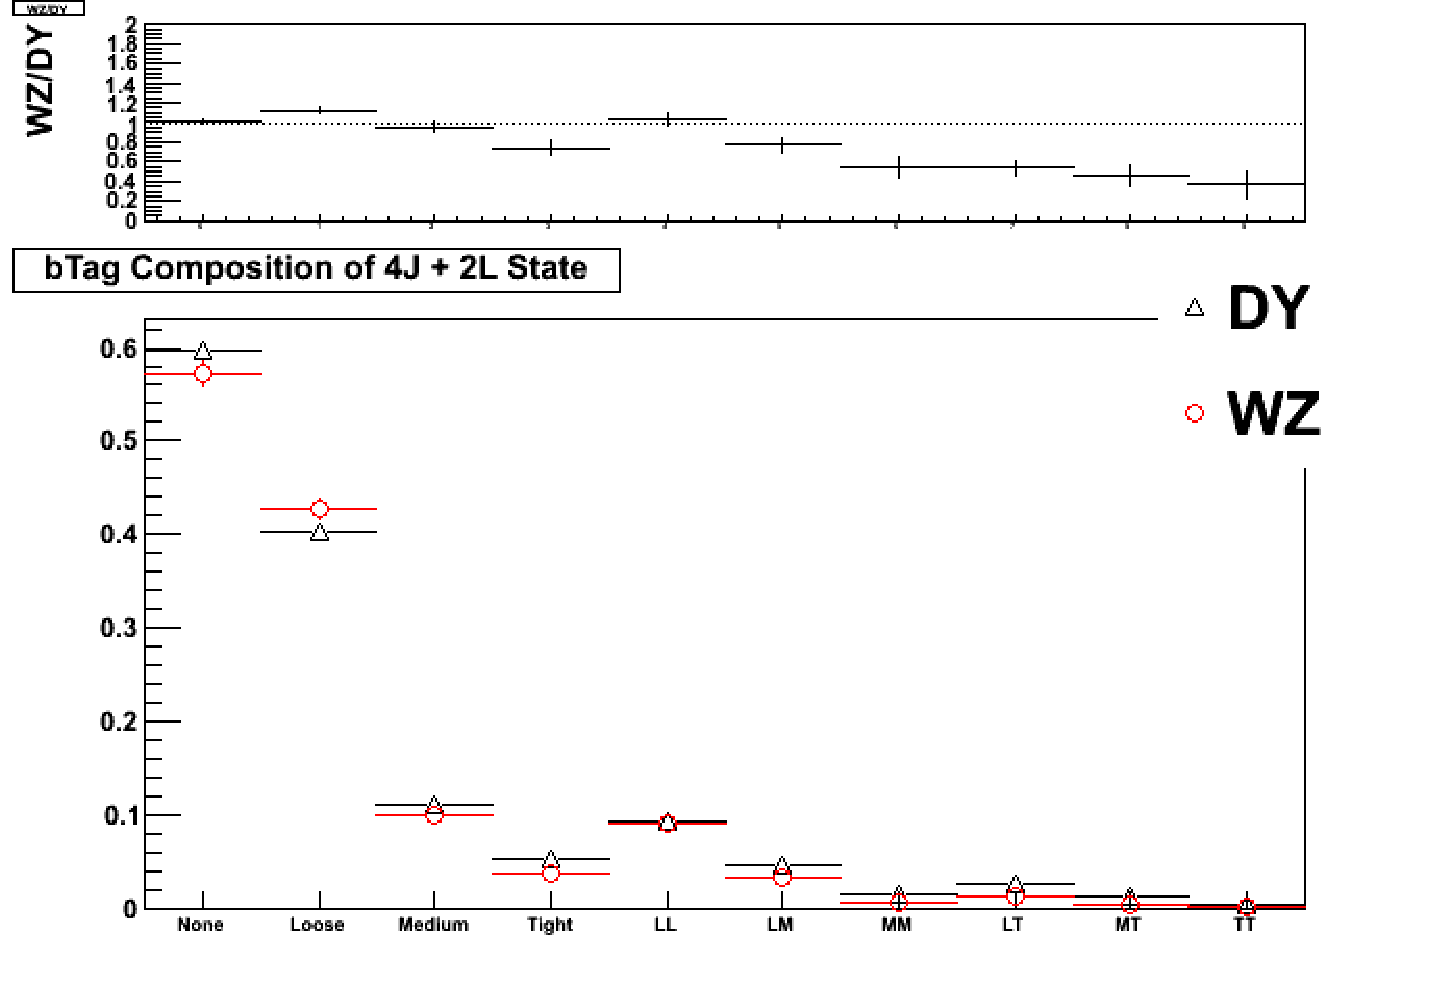
\includegraphics[width=0.90\linewidth]{Figs/WZ_Vs_DY_bComposition.pdf}
%\caption{\label{fig:wz_v_dy_btags}
%The b-tag composition of WZ and Z events in MC. In this plot, the first 2 bins (``None" and ``Loose") add up to the total number of events in the sample. The rest of the bins are a subset of the ``Loose" bin which shows the fraction of events with at least one CSV Loose b-tag. The bin labeled ``LL" means that this is the fraction of events with at least two CSV Loose b-tags. ``LM" means at least one Loose and one Medium, and so on. The WZ and Z samples are in good enough agreement for this purpose.
%}
%\end{center}
%\end{figure}

In data, control region events are required to pass the same mono- and di-lepton triggers as in the full analysis (there is a third lepton veto to make this region exclusive with the signal selection and thus the tri-lepton triggers are not used). The di-lepton event uses the same lepton requirements as are on the two leptons that are reconstructed as a Z in the tri-lepton selections in Section~\ref{sec:ElectronSelections}. Two mutually exclusive regions are defined, one with one CSV Loose b-tag and one CSV Medium b-tag used as the numerator of the ratio and one with a b-veto (i.e. zero Loose b-tags) used as the denominator of the ratio. These regions (particularly the b-tagged region) are contaminated with \ttbar \ events. A similar selection is made with the requirement that the di-lepton events contain two leptons that are different flavors (i.e. one electron and one muon), and this yield is subtracted from the Z like events to remove \ttbar \ contamination. The \ttbar \ estimate relies on the fact that the tops have final state decays into same flavor leptons at roughly the same rate as opposite flavor leptons. This creates a highly pure Z sample from which to determine the ratio. The constituents of the ratio are shown in both data and MC in Table ~\ref{tab:brate}

\begin{table}[ht!]
\caption{ \label{tab:brate} The constituent regions in the rate of b-tags in a 2L sample. An opposite flavor subtraction has been performed to create a more pure sample. Note the discrepancy between data and MC which will contribute to the systematic error on this method.}
\begin{center}
\begin{tabular}{c|cc}\hline
                                                         & 4J b-Veto                                & 4J (1Mb + 1Lb)\\
\hline \hline
W $\rightarrow \ell \nu$                       & 0.00$\pm$10.90      & 0.00$\pm$10.90    \\
VV $\rightarrow 2 \ell$                        & 951.43$\pm$4.30     & 216.37$\pm$2.15   \\
$t\overline{t}$                                & 2.40$\pm$2.37       & 5.48$\pm$7.80     \\
DY $\rightarrow 2 \ell$                        & 23678.13$\pm$224.34 & 2787.51$\pm$76.98 \\
%\hdashline
VZ $\rightarrow 3\ell$ or $4\ell$              & 28.38$\pm$0.50      & 3.65$\pm$0.17     \\
WWV                                            & 3.89$\pm$0.15       & 0.97$\pm$0.08     \\
%\hdashline
\ttX/tbZ/VZZ                                   & 5.21$\pm$0.26       & 10.00$\pm$0.80    \\
%\hdashline
\ttZ                                           & 3.48$\pm$0.26       & 33.97$\pm$0.83    \\
\hline \hline
Total from MC                                  & 24672.92$\pm$224.66 & 3057.94$\pm$78.18 \\
\hline
Data (19.5 fb$^{-1}$)                           & 24629.00$\pm$157.53 & 3874.00$\pm$75.54 \\
\hline
\end{tabular}
\end{center}
\end{table}
		
		
        		\subsubsection{Determining the Uncertainty in the Prediction from the b-tag Rate}
		A closure test on the accuracy of this method's predictions is performed in two ways. The first method is designed to show the integrity of the underlying assumption of the method that b-tag rates are independent of final states. The results are summarized in Table~\ref{tab:wz_z_brateclosure}. The rate of b-tags is measured in pure Z to two leptons with jets in MC and applied to a b-Veto region in our WZ, ZZ, and WWV samples with jets in MC. All three are included because they contribute and have enough statistics to be meaningful. This prediction is compared to the number of events measured in the two b-tag region for the pure WZ, ZZ, and WWV samples. The second test is designed to show the performance of the method in a sample with other types of processes than radiation producing jets that get b-tagged. The rate of b-tags is measured in a full cocktail of MC samples (with opposite flavor subtraction) with a two lepton and jets final state. This is then applied again to the WZ, ZZ, WWV samples with a three leptons and jets final state. The prediction is then compared to the measurement of three lepton and jets with b-tags in the same cocktail of MC. The results for the second test are summarized in Table~\ref{tab:mcsoup_brateclosure}.\\

\begin{table}[ht!]
\caption{ \label{tab:wz_z_brateclosure} Comparing the prediction of pure WZ, ZZ, and WWV MC events in a tri-lepton selection with b-tags from b-tag rates in pure Z MC sample.}
\begin{center}
\begin{tabular}{c|ccc}\hline
                                                                                               & Predicted            & Observed          & Pred. / Obs.\\
\hline \hline
WZ$\rightarrow 3\ell $ , ZZ$\rightarrow 4\ell$ , WWV  &  1.56$\pm$0.14 & 1.19$\pm$0.10 & 1.31$\pm$0.16\\		
\hline
\end{tabular}
\end{center}
\end{table}

\begin{table}[ht!]
\caption{ \label{tab:mcsoup_brateclosure} Comparing the prediction of pure WZ, ZZ, and WWV MC events in a tri-lepton selection with b-tags from b-tag rates in a cocktail of MC events in two lepton final state.}
\begin{center}
\begin{tabular}{c|ccc}\hline
                                                                                               & Predicted             & Observed          & Pred. / Obs.\\
\hline \hline
WZ$\rightarrow 3\ell $ , ZZ$\rightarrow 4\ell $ , WWV & $1.65 \pm 0.14$ & $1.19\pm0.10$ & $1.39 \pm 0.16$ \\
\hline
\end{tabular}
\end{center}
\end{table}

Based on the closure test results (Tables~\ref{tab:wz_z_brateclosure} and~\ref{tab:mcsoup_brateclosure}) and the agreement between data and MC shown in Table~\ref{tab:brate}, a 50\% systematic will be assessed on the prediction from this method.\\
		
		
        		\subsubsection{Predictions Due to the b-tag Rate Method}
		The columns from Table ~\ref{tab:brate} are used to predict the rate of b-tag events. The rate and the b-veto prediction region yields are listed in Table ~\ref{tab:brate_prediction} as well as the prediction.

\begin{table}[ht!]
\caption{ \label{tab:brate_prediction} Background predictions in data and MC for processes with b-tags that originate from radiation jets. Errors are statistical only.}
\begin{center}
\begin{tabular}{c|ccc}\hline
	   & Rate of b-tags	& Yields in b-Veto Sideband &	Bkg Prediction \\ \hline
Data   & 0.16$\pm$0.003	& 20.00$\pm$4.47            & 3.15+/-0.71 \\
MC	   & 0.12$\pm$0.003	& 14.38$\pm$2.45            & 1.78+/-0.31 \\
\hline
\end{tabular}
\end{center}
\end{table}

The prediction in Table~\ref{tab:brate_prediction} is further corrected by a scale factor determined by the Pred./Obs. in Table~\ref{tab:mcsoup_brateclosure}. The error remains the same, but the central value is now made better by correcting for the over prediction of the method. The final prediction is 2.27$\pm$0.51$_{st} \pm$1.14$_{sy}$.
		


\chapter{Efficiencies and Uncertainty}
\label{ch:eff_and_unc}

Systematic uncertainties on signal event selections arise from differences between simulated events and the actual performance of  the detector or slight differences in physical processes from simulated processes.

A summary of systematic uncertainties is given in Table~\ref{tab:systSumm}. Full descriptions of each systematic are presented in the following sub-sections.

\begin{table}[h]
\begin{center}

\begin{tabular}{lcccc}\hline
Source 					& Method & Total Systematic 	\\ \hline
Jet Energy Scale			& Momentum Scale Up/Down                        & 4.8\%	\\
Jet Energy Resolution	                   	& Momentum Smearing                                         & 0.4\%	\\

b-tag (light flavor)                          & Discriminant Re-weight                              & 1.0\%       	\\
b-tag (b flavor)		                      & Discriminant Re-weight                              & 2.9\%	\\	
Q$^2$                                         & Q$^2$ Scale Up/Down                                 & 1.7\% \\
Matching                                      & Matching Scale Up/Down                              & 1.2\% \\
Top Mass                                      & Mass Scale Up/Down                                  & 2.5\% \\
PDF				                              & PDF Re-weight                                       & 1.5\%	\\
Generator                                     & Compare 2 ttZ Samples                               & 5.0\% \\
Pile Up                                       &                                                     & 1.0\% \\
Trigger                                       &                                                     & \lt 1\% \\
Lepton Identification, Isolation,             & Tag \& Probe                                        & 6.2\% \\
and Event Composition  & & \\
\hline
Total 					                                                                             & & 10.5\% 	\\
\hline
\end{tabular}
\caption{\label{tab:systSumm}Summary of systematic uncertainties on the signal selection and
expectation. 
Reported values are fractional, relative to the total cross section.}
\end{center}
\end{table}

\section{Lepton MC to Data Scale Factors and Uncertainties}
\label{sec:tag_and_probe}

Data-Monte Carlo scale factors are derived using the leptonic identification and isolation requirement efficiencies measured with the ``tag and probe" method. The method identifies dilpeton Z events from the full 2012 dataset. One lepton, known as the ``tag," passes the complete set of lepton selections. The other lepton, known as the ``probe," is allowed to pass a relaxed set of requirements. In the case of measuring the efficiency of the isolation requirement, the probe is required to pass the full identification and quality cuts but not the isolation. The efficiency is the ratio of probes passing the isolation requirement to those not passing the requirement. In the case of measuring the efficiency of the identification requirement, the probe is required to pass the full isolation cut but not the identification cuts. \\

For electrons, the tag is required to be matched to the \verb=HLT_Ele27_WP80= trigger, which requires one well-identified electron passing the WP80 electron ID~\cite{egammaidtwiki} with \pt \gt 27 \GeV. The tag electron must also pass the electron identification requirements and isolation cut in Sec~\ref{sec:ElectronSelections}. The \pt \ threshold of the tag electron is additionally raised to 32 \GeV \ to avoid trigger turn-on effects. The probe electron has a base requirement of
\begin{itemize}
\item \pt \gt 10 \GeV 
\item $|\eta| \lt 2.4$, and excluding electrons with a supercluster between $1.4442 \lt |\eta| \lt 1.566$
\end{itemize}
The identification efficiency is measured with the probe electron additionally passing the isolation requirements described in Sec~\ref{sec:ElectronSelections} but not the identification requirements. The derived efficiency is directly applicable to the leptons in the full tri-lepton analysis as identification requirements are a property of the lepton alone. The isolation efficiency, however, is dependent on the energy (mainly energy from hadronic activity) in the event. As such, both the electron identification and an additional jet selection is required matching those described in Sec~\ref{sec:JetSelection}. The overall electron efficiency may be measured by relaxing the probe electron to the nominal value. The electron efficiencies are summarized in Table~\ref{tab:eleffiency}. A simultaneous fit is performed on the di-lepton data in the invariant mass range of $60-120 \ \GeV$ using models from Table~\ref{tab:tnpmodels} selected for performance on a bin-by-bin basis. This becomes necessary as the kinematics varies with \pt \ and \aeta \ bins and fitting models must be chosen for best results.\\

\begin{table}[h]
\begin{center}

\begin{tabular}{l|c}\hline
 Model                                                                               & Usage \\ \hline \hline
 Breit-Wigner function $\star$ Crystal-Ball function & Signal \\
 MC-based template function                                       & Signal \\
 Exponential                                                                    & Background \\
 Exponential $\star$ Error function                             & Background \\
 Polynomial                                                                     & Background \\
 Polynomial $\times$ Exponential function               & Background \\
 Chebyshev Polynomial                                               & Background \\
\end{tabular}
\caption{\label{tab:tnpmodels} Models used for fitting the signal or the background contribution in the tag and probe method.}
\end{center}
\end{table}

\begin{sidewaystable}[h]
\begin{center}

\begin{tabular}{c|c|c|c|c|c} \hline \hline
\pt - $|\eta|$   &                 &20 - 30 \GeV & 30 - 40 \GeV & 40 - 50 \GeV & 50 - 200 \GeV \\ \hline
%                        & MC          &  &  & \\
%                        & Data       & & & \\
0.0 - 0.8         & Data/MC & 0.947 +/- 0.003 & 0.963 +/- 0.001 & 0.975 +/- 0.001 & 0.973 +/- 0.001 \\ \hline
%                        & MC          & & & \\
%                        & Data       & & & \\
0.8 - 1.4442   & Data/MC & 0.885 +/- 0.004 & 0.942 +/- 0.001 & 0.960 +/- 0.001 & 0.962 +/- 0.001 \\ \hline
%                         & MC          & & & \\
%                         & Data       & & & \\
1.566 - 2.0      & Data/MC & 0.928 +/- 0.016 & 0.936 +/- 0.002 & 0.959 +/- 0.001 & 0.969 +/- 0.002\\ \hline
%                         & MC          & & & \\
%                         & Data       & & & \\
2.0 - 2.4          & Data/MC & 0.994 +/- 0.006 & 0.980 +/- 0.003 & 0.982 +/- 0.002 & 0.978 +/- 0.004 \\ \hline \hline
\end{tabular}
\caption{ \label{tab:eleffiency} Measured electron efficiency ratios using the tag and probe method. Errors are statistical only.}
\end{center}
\end{sidewaystable}

Muon identification and isolation requirement efficiencies are measured using the same methods as with the electrons. Appropriate muon specific identification and isolation requirements as described in Sec~\ref{sec:MuonSelections} are used instead of the electron specific ones above.\\

\begin{sidewaystable}[h]
\begin{center}

\begin{tabular}{c|c|c|c|c|c} \hline \hline
\pt - $|\eta|$ &                 &20 - 30 \GeV & 30 - 40 \GeV & 40 - 50 \GeV & 50 - 200 \GeV \\ \hline
%                      & MC          &  &  & \\
%                      & Data       & & & \\
0.0 - 1.20     & Data/MC & 0.962 +/- 0.001 & 0.972 +/- 0.001 & 0.978 +/- 0.000 & 0.974 +/- 0.001 \\ \hline
%                      & MC          & & & \\
%                      & Data       & & & \\
1.20 - 2.50   & Data/MC & 0.974 +/- 0.002 & 0.978 +/- 0.001 & 0.984 +/- 0.000 & 0.978 +/- 0.001 \\ \hline \hline
\end{tabular}
\caption{ \label{tab:mueffiency} Measured muon efficiency ratios using the tag and probe method. Errors are statistical only.}
\end{center}
\end{sidewaystable}

\clearpage

For both the electrons and muons, the Tag and Probe measurements were repeated in two ways. The first measured the scale factor by allowing the probe to fail both ID and ISO requirements. The second allowed the probe to fail ID or ISO requirements separately, and the two scale factors were multiplied together. The difference in scale factor between those derived by allowing both ID and ISO to fail together and those derived by combining two measurements that allowed ID and ISO to fail individually is used to assess a systematic uncertainty in this procedure. An average value of deviation across the bins is chosen. In this case, we use 1.5\% on electrons and 0.3\% on muons in addition to the statistical errors quoted in the tables.

Additionally, the  measurements are performed in a pure Drell-Yan sample and may differ slightly for the isolation requirements from those in the analysis selections due to hadronic activity. A study in pure MC was performed to compare the isolation values of electrons or muons generator matched to a status three electron or muon. A Drell-Yan sample and a \ttZ \ sample were chosen for this comparison and listed in Appendix~\ref{sec:mc_details}. The isolation curves are compared for leptons from both samples by looking at the fraction of events passing the isolation cut. This is done by comparing DY sample with no Jet multiplicity requirement to a \ttZ \ sample requiring four Jets.  The difference between the fractions  additional systematic is assessed due to the difference in efficiency for the respective analysis isolation cuts between the two samples. Leptons are required to pass the acceptance selections, $\pt > 20 \GeV$, and full identification selections as defined in Sec~\ref{sec:EventSelections}. For muons and electrons the difference is 2\%.

Finally, the scale factors in Tables~\ref{tab:eleffiency} and~\ref{tab:mueffiency} are used to reweight MC events based on the identified leptons. To determine the total amount of uncertainty due to the lepton efficiencies, the scale factors are varied up and down by their total errors (stat and systematic). The electron errors and muon errors are assumed to be uncorrellated and thus varied independently between the two. The hadronic activity error is considered correlated for both flavors and varried at the same time for both flavors. The difference between the yields of the up and down variations is used to determine a systematic uncertainty on lepton efficiency, and the three variations (e, $\mu$, hadronic) are added in quadrature. This uncertainty is 6.2\% and is summarized in Table~\ref{tab:systSumm}.\\\\





\section{Systematic Uncertainty Due to Triggers}   
\label{sec:trigger_syst}
Dilepton triggers are used with a selection that ultimately chooses three leptons. This means that the triggers are ultra-efficient as only 2/3 of the leptons need to be identified by the triggers. We assign a 1\% uncertainty to cover the nearly negligible chance of a three lepton event failing a dilepton trigger.

\section{b-tagging Efficiency and Associate Errors}
\label{sec:btag_syst}
b-tagged jets are chosen based on CSV discriminant thresholds. Differences arise in the shape of the discriminant distributions in Data and MC. In the past event weights were scaled to account for this and match up the number of b-tags in Data and MC. Another current method involves promoting or demoting b-tagged jets (e.g. CSVL to None or CSVM to CSVT) using random numbers. This method has the drawback that it becomes fairly complicated to perform when using more than one threshold (e.g. requiring one CSVL and one CSVM b-tagged jets). A more natural and fitting method reshapes the MC discriminant distribution. This has the advantage of preferentially promoting or demoting b-jets on the border of a threshold and removing any complexities arising from multiple levels of tightness. The BTV POG recommended methods are summarized for use in reference~\cite{bTagSF}.\\

The discriminant is reshaped based on Data/MC scale factors measured in~\cite{BTV11003} by the BTV POG for both light flavor jets mis-tagging and b-jets tagging. Signal systematics are then determined by reshaping the MC discriminant with the scale factors varied up and down by the error on the scale factor measurement. The MC FlavorAlgo values are used for the jet to quark truth matching. This variation is performed in the \ttZ \ signal sample listed in Sec~\ref{sec:mc_details}. The percentage difference up and down from the central value is then chosen as the error. This is done separately and independently for both the light flavor scale factors and the b scale factors. The two errors are added in quadrature to get a total (see Table~\ref{tab:systbTag}).


\begin{table}[h]
\begin{center}

\begin{tabular}{lc}\hline
Source & Total Systematic \\ \hline
b Quarks & 2.9\% \\
Light Flavor Quarks & 1.0\% \\ \hline
Total & 3.1\% \\
\hline
\end{tabular}
\caption{\label{tab:systbTag} Summary of systematic b-tag uncertainties split by light flavor and b contributions.}
\end{center}
\end{table}



%\chapter{Other Uncertainties Due to Use of Simulations}
\section{Uncertainties  Involved in Event Generation}
The previous chapter was concerned with uncertainties due to reconstructed and identified quantities in the MC simulations. The following chapter will discuss uncertainties in the simulation at a lower level, at the level of event generation. These can come from the parton distribution functions used, masses used for particles, or the order to which calculations are performed.\\ 

\subsection{Uncertainties Due to Parton Distribution Functions}	
Proton-proton interactions are not as straightforward as single particle interactions (e.g. electron-electron). Although the theory for quarks interacting or gluons interacting is well understood, interaction between composite objects are much more complicated. Parton Distribution Functions enter to help describe the probability density of finding a particular particle inside the proton with a certain longitudinal momentum fraction at a specific resolution (Q$^2$). Due to the non-perturbative nature of the partons which are not seen as free particles, this cannot be calculated via perturbative QCD. External methods must be used to probe the structure and distribution of the proton. This measured structure can then be used within a theoretical framework. Experimental error must be assessed to determine the impact of choosing different PDFs for the MC simulations.\\

The recommendations of the PDF4LHC~\cite{PDF4LHC} group are followed for estimating the acceptance uncertainty from the PDF. The predictions from CT10, MSTW, and NNPDF sets are used. The LHAPDF package is used for PDFs and the re-weight function. Each set and all of its error subsets are run over and used to re-weight the \ttZ \ MC to determine an acceptance. MC events are re-weighted from the generator PDF (CTEQ6) to the variation based on the parton type and momentum.\\

\subsubsection{CT10}
The PDF uncertainty for CT10 is calculated by

\begin{equation}
\Delta A^{+} = \sqrt{ \displaystyle \sum \limits_{i=1}^N [	\max(A_i^{+} - A_0, A_i^{-} - A_0, 0) ] ^ 2},
\end{equation}

\begin{equation}
\Delta A^{-} = \sqrt{ \displaystyle \sum \limits_{i=1}^N [	\max(A_0 - A_i^{+}, A_0 - A_i^{-} , 0) ] ^ 2},
\end{equation}
where $A_0$ is computed with the central PDF, i runs over the error sets, $A^{+}$ and $A^{-}$ denote the up and down errors respectively on the acceptances of the ith eigenvector subset. The $\alpha _s$ uncertainty is obtained by considering PDFs for $\alpha _s$ = 0.116, 0.117, 0.118, 0.119, 0.120. The same equations above are applied to these subsets. Finally, it is noted that the PDFs for CT10 are at 90\% CL variations and thus the results are scaled down by 1.645 to obtain the 68\% CL uncertainty.
	
\subsubsection{MSTW}
Five different sets are used for MSTW with $\alpha _s = \alpha _s ^ 0$, $\alpha _s ^ 0 \pm 0.5 \sigma$, and $\alpha _s ^ 0 \pm \sigma$. The uncertainty is given with the following formulae:
\begin{equation}
\Delta A^{+} = \underset{\alpha _s}{\max} [ A_{\alpha _ s} + \Delta A_{\alpha _s} ]  - A_0,  
\end{equation}

\begin{equation}
\Delta A^{-} = A_0 -  \underset{\alpha _s}{\max} [ A_{\alpha _ s} - \Delta A_{\alpha _s} ], 
\end{equation}
where $A_0$ is from the central value PDF.\\

\subsubsection{NNPDF2.0}
The NNPDF samples of PDF+$\alpha _s$ is obtained by using NNPDF sets with different fixed $\alpha _s$ corresponding to a Gaussian sample around the nominal $\alpha _s = 0.119$ as shown in Table~\ref{tab:nnPDFsets}.
 
\begin{table}[h]
\caption{\label{tab:nnPDFsets} Number of NNPDF replicas for each $\alpha _s$.}
\begin{center}
\begin{tabular}{c|ccccccc}\hline
$\alpha _s$         &  0.116 & 0.117 & 0.118 & 0.119 & 0.120 & 0.121 & 0.122 \\ \hline
$N_{rep}$                &  5         &  27      &  72      &   100   &  72     &   27    &    5       \\
\hline
\end{tabular}
\end{center}
\end{table}

The uncertainty is computed using the following equations:

\begin{equation}
\Delta A ^{+} = \sqrt{  \frac{1}{N^{+} - 1} \sum \limits_{i=1}^{N^{+}} (A_i - A_0)^2},
\end{equation}
\begin{equation}
\Delta A ^{-} = \sqrt{  \frac{1}{N^{-} - 1} \sum \limits_{j=1}^{N^{-}} (A_0 - A_j)^2},
\end{equation}
with $A_0$ computed front he central value PDF at $\alpha = 0.119$, i running over the $N^{+}$ replicas where $A_i$ \gt $A_0$, and j running over the $N^{-}$ replicas with $A_j$ \lt $A_0$.\\

\subsubsection{Combined Results}
To combine the measurements into one error, the uncertainty is computed with the following equations:

\begin{equation}
\Delta _{\max} = \underset{i}{\max}  [A_i + \Delta A^{+} _i],
\end{equation}
\begin{equation}
\Delta _{\min} = \underset{i}{\min}  [A_i - \Delta A^{-} _i],
\end{equation}
and the PDF uncertainty is
\begin{equation}
Unc_{PDF} = \frac{1}{2}(\Delta _{max} - \Delta _{min} ),
\end{equation}
where i runs over all of the PDF sets listed above.\\

Using this procedure, yields an uncertainty of 1.5\%.



\subsection{Uncertainties Measured in Top Samples}
A number of uncertainties are measured by varying parameters in top samples. Ideally, these parameters should be varied in a \ttZ \ sample, but since none were produced centrally by CMS, already existing \ttbar samples were used with analogous cuts to the \ttZ \ analysis. that is one lepton was selected, two b-tagged jets, and an additional two jets. These samples are listed in Table~\ref{tab:sampleupdown}.

\begin{table}[h]
\caption{\label{tab:sampleupdown} List of alternate \ttbar \ samples scaling up or down relative parameters to the systematics. Summer12\textunderscore DR53X-PU\textunderscore S10\textunderscore START53\textunderscore V7A-v1 is replaced by SU12 for brevity.}
\begin{center}
\begin{tabular}{l}\hline
Sample   \\ \hline
 \verb=/TTJets_mass178_5_TuneZ2star_8TeV-madgraph-tauola/SU12/AODSIM=   \\
 \verb=/TTJets_mass166_5_TuneZ2star_8TeV-madgraph-tauola/SU12/AODSIM=   \\  %\hdashline
 \verb=/TTJets_scaleup_TuneZ2star_8TeV-madgraph-tauola/SU12/AODSIM=  \\
 \verb=/TTJets_scaledown_TuneZ2star_8TeV-madgraph-tauola/SU12/AODSIM=  \\ %\hdashline
 \verb=/TTJets_matchingup_TuneZ2star_8TeV-madgraph-tauola/SU12/AODSIM=  \\
 \verb=/TTJets_matchingdown_TuneZ2star_8TeV-madgraph-tauola/SU12/AODSIM=  \\
\hline
\end{tabular}
\end{center}
\end{table}

In order to use the \ttbar \ samples, the full analysis selections must be modified to become a mono-lepton selection instead of a tri-lepton selection, so that only prompt leptons are considered and the jet production methods remain the same. In essence this just removes the Z selection. There is an additional benefit from this modified selection in that it creates a high statistics region to derive the systematic errors. The number of events passing the modified selections in each sample are compared to the number of generator level events with 1 lepton. The /TTJets\_SemiLeptMGDecays\_8TeV-madgraph/Su12\_V7A\_ext-v1/AODSIM  (where Su12 stands for Summer12\_DR53X-PU\_S10\_START53) sample is used to produce a central value, and the fraction passing from the varied samples is compared to the fraction passing from the central value to determine the systematic error on each variation. The results are summarized in Table ~\ref{tab:systupdown}.

\subsubsection{Uncertainties Due to Parton Momentum Transfer}
Proton structures can be probed with electrons and the inelastic scattering follows a scaling known as Bjorken scaling. This scaling depends on the momentum transfer produced by the photon force carrier in the interaction. This momentum is in the form of a 4-vector and included in the scaling as a quadratic (written as Q$^2$).\\

\subsubsection{Uncertainties Due to Top Mass}
The top mass is measured as $173.21 \pm 0.51 \pm 0.71$ \GeV~\cite{pdg}. However, due to the size of the error on the mass, it's impact on simulated samples must be evaluated. This mass is varied up and down in simulation production by a range wider than that of the error in order to gauge its impact.\\


\subsubsection{Uncertainties Due to Matching}
Matching is a process that occurs between the Matrix Element simulation of the underlying event and the parton showering afterwards. Generally these two steps are handled by different pieces of software. At NLO level this is difficult because a scheme must be used to prevent double counting. At LO level this process can be highly dependent on jet resolution. Again, the best way to identify the impact on the uncertainty due to matching is by varying the matching scheme in simulated samples.\\


\begin{table}[h]
\caption{\label{tab:systupdown} Summary of systematic b-Tag uncertainties split by light flavor and b contributions. Note: Half the error established by varying the top mass is used because the mass range is much wider than the current considered error on the top mass measurement.}
\begin{center}
\begin{tabular}{lccc}\hline
Source                  &  N Pass / N Gen & \% Deviation from Central & Notes\\ \hline
Central                 & 0.265 & & \\
Q$^2$ Up                 & 0.261 & -1.5\% & \\
Q$^2$ Down           & 0.270 & 1.8\% & \\
Matching Up       & 0.261 & -1.6\% & \\
Matching Down  & 0.267 & 0.8\% & \\
Mass 166.5         & 0.251 & -5.2\% & Use half \\
Mass 178.5         & 0.277 & 4.5\% & Use half \\
\hline
Total                     &             & 3.3\% & Used half of\\
                              &             &             & Mass variation \\
\hline
\end{tabular}
\end{center}
\end{table}



\subsection{Uncertainties Due to Generators}	

The MC samples used in this analysis are primarily generated with the Madgraph event generator. Madgraph produces events at Leading Order. This may lead to a change in acceptance of the events compared to an NLO or NNLO event generator which comes into play with the signal acceptance. Despite the general belief that NLO samples are more accurate, Madgraph samples were still chosen here due to the inconsistent widespread availability of aMC@NLO samples as well as the fact that the available \ttZ \ and \ttW \ aMC@NLO were produced without final state photon radiation. To study this potential uncertainty, two \ttZ samples are used and are summarized in Table~\ref{tab:App:ttZGeneratorMCs}. The first is a Madgraph~\cite{Alwall:2011uj} sample which is used elsewhere in the analysis. The second is an aMC@NLO (~\cite{Frederix:2011zi, Frederix:2011ss} based on the MC@NLO formalism~\cite{Frixione:2002ik} and the MadGraph5 framework~\cite{Alwall:2011uj}) sample. \\




For each sample an efficiency ($\epsilon$) is prepared. The efficiency is defined as
\begin{equation}
\epsilon = \frac{n\ with\ 3\ leptons\ and\ 4\ jets}{n\ with\ 3\ leptons}.
\end{equation}

The exact selections for the denominator are:
\begin{itemize}
\item Exactly three status 3 generator leptons (electrons or muons)
\item All of the above generator leptons with \pt \gt 20 \GeV and \aeta \lt 2.4.
\item All of the above generator leptons came from a W or a Z.
\item Exactly three reconstructed leptons (electrons or muons) that pass the identification and isolation selections in Sec~\ref{sec:EventSelections}
\item Reconstructed leptons that do not match the generator leptons above are rejected.
\end{itemize}

The exact selections for the numerator are:
\begin{itemize}
\item Denominator as above.
\item At least four pfJets with applicable energy corrections with \pt \gt 20 \GeV and \aeta \lt 2.4. 
\item Jets within a cone 0.5 of a lepton identified in the numerator are rejected.
\item Jets with \lt 10\% of their energy coming from the primary vertex are rejected.
\end{itemize}

Then the difference is defined as
\begin{equation}
\Delta = \left| 1 - \frac{\epsilon _{aMC@NLO}}{\epsilon _{Madgraph}} \right|
\end{equation}
and the results are summarized in Table~\ref{tab:systgeneratorsum}

\begin{table}[h]
\caption{\label{tab:systgeneratorsum} Summary of the efficiencies using the Madgraph and aMC@NLO event generators for the jet selections.}
\begin{center}
\begin{tabular}{ccc}\hline
Madgraph           &  aMC@NLO & Difference \\ \hline
0.38                      & 0.36              & 5\%\\
\hline
\end{tabular}
\end{center}
\end{table}

After evaluating and comparing the efficiencies, The contribution to the signal uncertainty from the generator calculation order is set at 5\%.

\section{Jet Energy Scale and Resolution}
Jets are experimental signatures at particle detectors that seek to cluster together showering particles that came from a single source and treats that cluster as a composite object for the sake of the measurements. The accuracy of the energy in this jet are determined by both resolution and scale. The jet energy resolution is a determination of the spread of the distribution of the pull of the energy (pull = true - measured). This resolution is different between data and simulation and simulation must be corrected to be more accurate. This also introduces an uncertainty which must be assessed. Jet energy scaling seeks to address any systematic biases in the jet energy measurement and scales the measured energy by factors to correct it. There is still an associated uncertainty on the jet energy and the contribution of this due to the scale must also be measured.\\

The jet energies have been corrected in data with a residual correction factor to account for differences between measured jet energies in data and in Monte Carlo~\cite{jes_ref}. These corrections come with uncertainties and thus matter for the signal acceptance. To account for this, we vary the jets' transverse momenta up and down by the one standard deviation uncertainties and compare the change in predicted yields in MC. The resultant uncertainty is 4.8\% and is listed in Table~\ref{tab:systSumm}.\\

The recommended prescription for determining uncertainty on the energy resolution of particle flow jets is outlined in~\cite{jer_ref}. Using signal Monte Carlo, the prescription was applied as follows:
\begin{itemize}
\item Each reconstructed jet is matched to the closest generator jet within a cone of $\Delta R < 0.5$.
\item If a match is found the transverse momentum of the reconstructed jet is scaled by.
\begin{equation}
\pt \rightarrow max \left[0, \pt ^{gen} + c \times \left(\pt - \pt ^{gen} \right) \right]
\end{equation}
where $\pt ^{gen}$ is the transverse momentum of the matched generator jet, and c is the data/MC scale factor between the measured and expected particle flow jet resolution in Table~\ref{tab:jer_scalefactor}.
\item If no match is found a gaussian centered at unit and with a width of $c$ is used to smear the momentum instead.
\end{itemize}

\begin{table}[h]
\caption{ \label{tab:jer_scalefactor} Data/MC scale factors used in determining the Jet Energy Resolution.}
\begin{center}
\begin{tabular}{c|c}\hline
Jet Pseudorapidity & Scale Factor \\ \hline \hline
0.0 - 0.5 & 1.052 \\
0.5 - 1.1 & 1.057 \\
1.1 - 1.7 & 1.096 \\
1.7 - 2.3 & 1.134 \\
2.3 - 5.0 & 1.288 \\
\hline
\hline
\end{tabular}
\end{center}
\end{table}

To determine the systematic uncertainty on this procedure, up and down variations (Table~\ref{tab:jer_scalefactor_updown}) on the scale factor c are used. The yields in \ttZ \ signal MC are determined with the central value of c as well as the up and down values. The uncertainty is given by
\begin{equation}
\mathrm{uncertainty} = \left| \frac{Yield _{up} - Yield _{down}}{Yield _{central}} \right|.
\end{equation}

\begin{table}[h]
\caption{ \label{tab:jer_scalefactor_updown} data/MC up/down scale factors used in determining the systematic uncertainty on Jet Energy Resolution.}
\begin{center}
\begin{tabular}{c|c|c}\hline
Jet Pseudorapidity & Scale Factor (UP) & Scale Factor (DOWN)\\ \hline \hline
0.0 - 0.5 & 1.115 & 0.990 \\
0.5 - 1.1 & 1.114 & 1.001 \\
1.1 - 1.7 & 1.161 & 1.032 \\
1.7 - 2.3 & 1.228 & 1.042 \\
2.3 - 5.0 & 1.488 & 1.089 \\
\hline
\hline
\end{tabular}
\end{center}
\end{table}

After following this procedure, the acceptance systematic due to Jet Energy Resolution is found to be 0.4\%. This result is summarized in Table ~\ref{tab:systSumm}.\\

\section{Pile Up}
In the LHC, large bunches of protons collide at a rapid rate. The rate of bunch crossings can theoretically be pushed to near the threshold of timing for the machine's electronics which can lead to residual energy still being measured in the detector from a previous collision during the current collision. This is called ``out of time pile up'' and is not an issue at the current rate of collisions for the LHC. Another form of pile up, known as ``in time pile up'' is an issue and is caused by multiple protons colliding within the crossing bunches.\\ 

Proton collisions are frequent, but collisions that produce interesting outcomes are not. So the LHC allows many collisions to happen at once in hopes that one will be interesting. In time pile up occurs when one proton collision produces an outcome that physicists would like to study, but at the same time other collisions produce uninteresting outcomes that nevertheless add energy into the detector which may alter the appearance of the decay products of the collision that physicists want to investigate.\\

Several techniques are employed to mitigate this affect in the jet clustering algorithms, jet energy measurements, and the lepton energy measurements with most of the techniques reducing to some level of subtracting an average ambient energy which has been measured in minimum bias events. However, this still produces some level of uncertainty in the current measurements, and can matter for event acceptance (for example when determining the amount of energy in a cone around a lepton for an isolation measurement).\\

To evaluate this level of uncertainty, Monte Carlo samples are compared to data in the selection region. The number of vertices in the events are measured, and the Monte Carlo events are reweighed to have the same distribution of vertices as the data events. From here total cross section of minimum bias events is varied up and down by 5\% when reweighing the Monte Carlo samples. The effect on the signal yield is found to be $\pm 5\%$ after full selections.


\chapter{\ttZ Cross Section Measurement}
The components of a measurement have been shown. Selections have been determined to identify a \ttZ \ production decaying to three leptons and jets and reduce the selection of background events. Methods for predicting the contributions to the selected events from the backgrounds have been developed. Finally the contribution of systematic uncertainties from the use of Monte Carlo simulations have been assessed. The following chapter applies the already developed selections to a data sample and combines the various pieces of the measurement into a cross section for the \ttZ \ production.\\

         \section{Data and Prediction Agreement in Preselection}

         The background prediction methods were developed with a high reliance on MC simulation to determine the behavior of the prediction methods. In the ideal scenario an independent region would be chosen in data to demonstrate the accuracy of the predictions. However, such a scenario is not feasible with the selections used for the \ttZ measurement. The next best option is to relax the selections and show that the predictions work in a looser signal region. Here a preselection is shown to demonstrate the agreement between the full data driven predictions and data. This region is composed of the full signal selections with the jet requirements loosened to two or more jets from the signal selection of four. This is done to be able to preserve the b-tags requirement. What results is a region with almost twice the events of the signal region and slightly enhanced backgrounds, both being useful to help illustrate the agreement of the predictions and data. WZ is a dominant background and thus the reconstructed mass of the Z and the \Mt \ of the W (Fig~\ref{fig:hmass_3L2b}) are good variables for comparison. Additionally, in the preselection region, it is possible to view a more complete picture of the jet multiplicity (Fig~\ref{fig:jetmult_3L2b}) which is important as this is used in the full selection. Finally, other distributions such as the lepton \pt \ are shown in Appendix~\ref{app:figures}. In the following plots, the irreducible background is taken from pure MC where the events have been scaled by lepton efficiency data to MC scale factors and the similar b-tagging efficiency scale factors. The luminosity is scaled to that of data. For the data driven predictions, the shape is taken from MC while the normalization of the background is from the data driven predictions in Sec~\ref{sec:datadriven}.


\begin{figure}[h]
\begin{center}
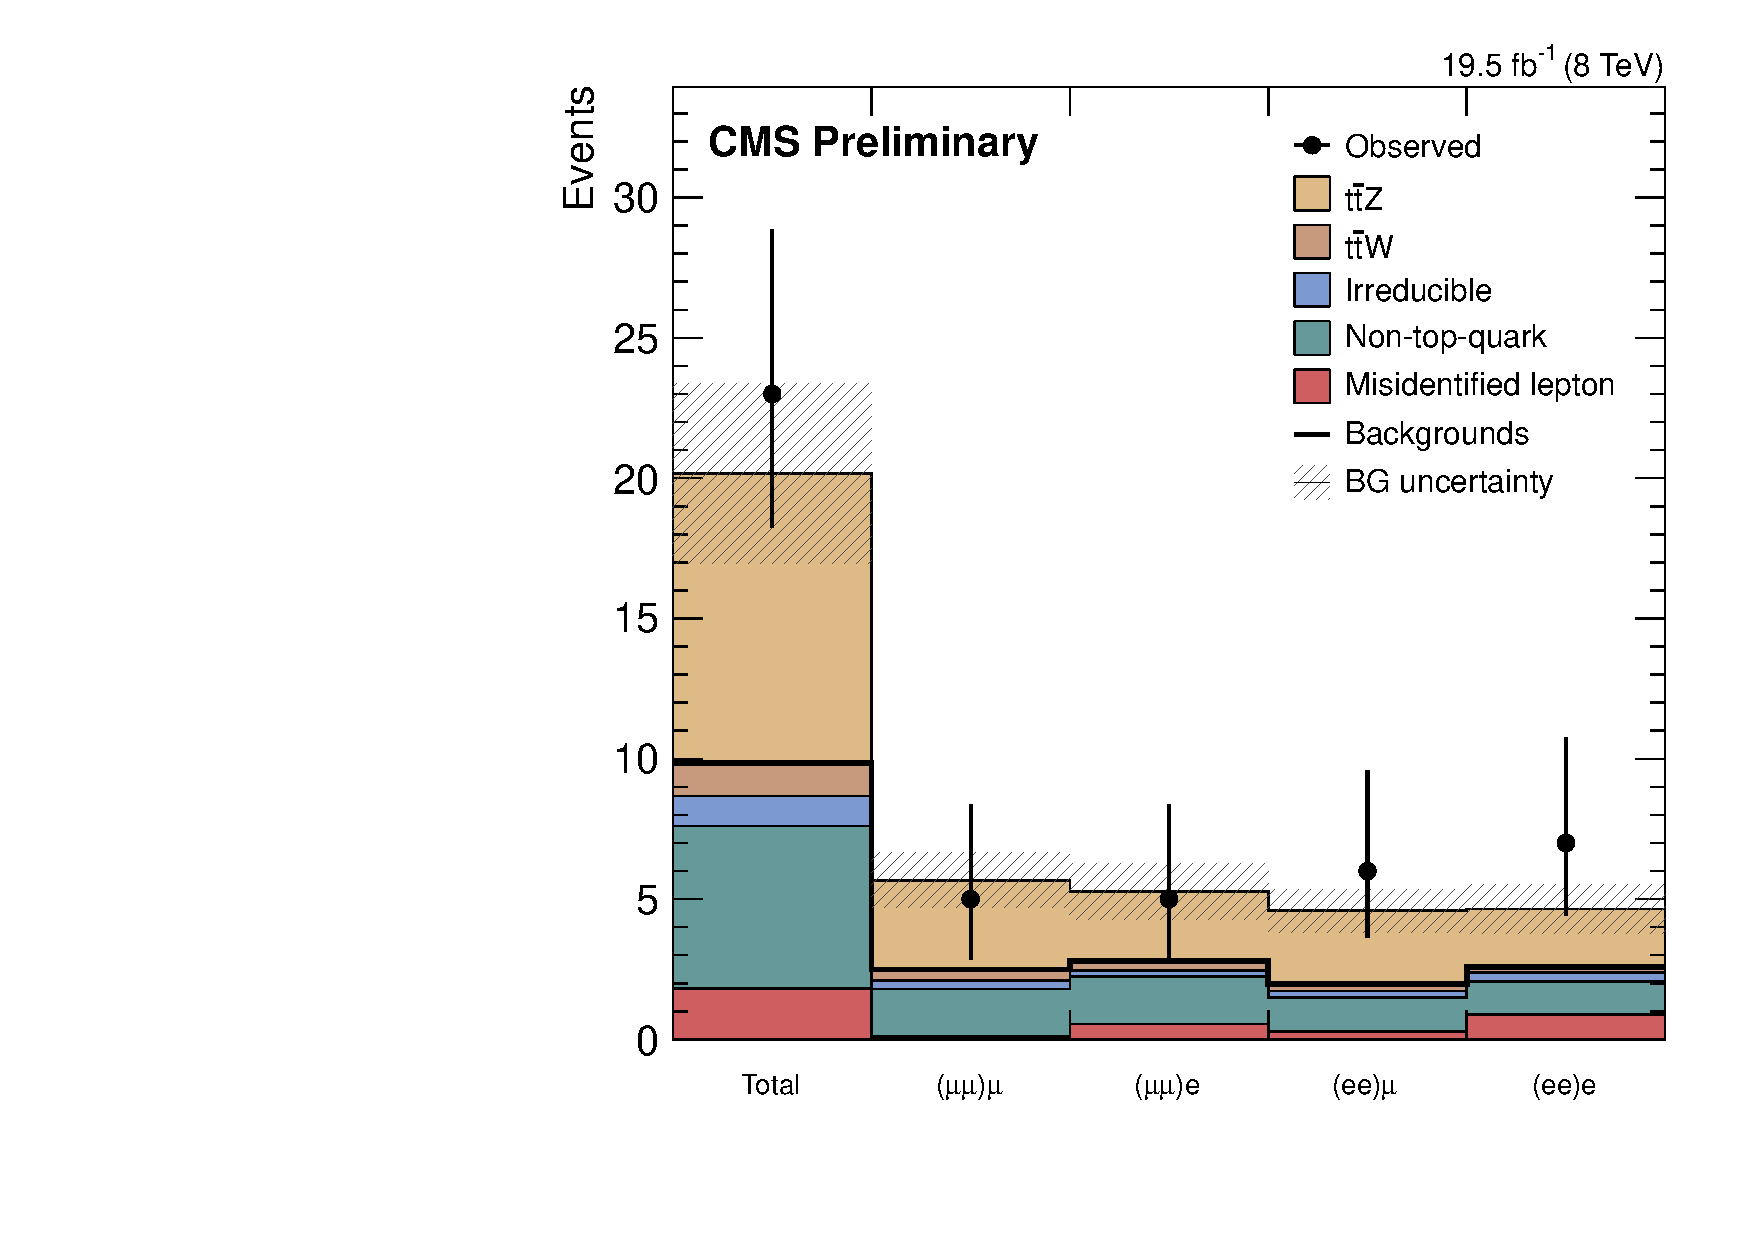
\includegraphics[width=0.7\linewidth]{Figs/Plots_PreSelections/hYields_3L2b.pdf}
\caption{\label{fig:hyields_3L2b}
Yields with break down by leptonic channel of data and predictions after tri-lepton plus two b-tag selections.
}
\end{center}
\end{figure}

\begin{figure}[h]
\begin{center}
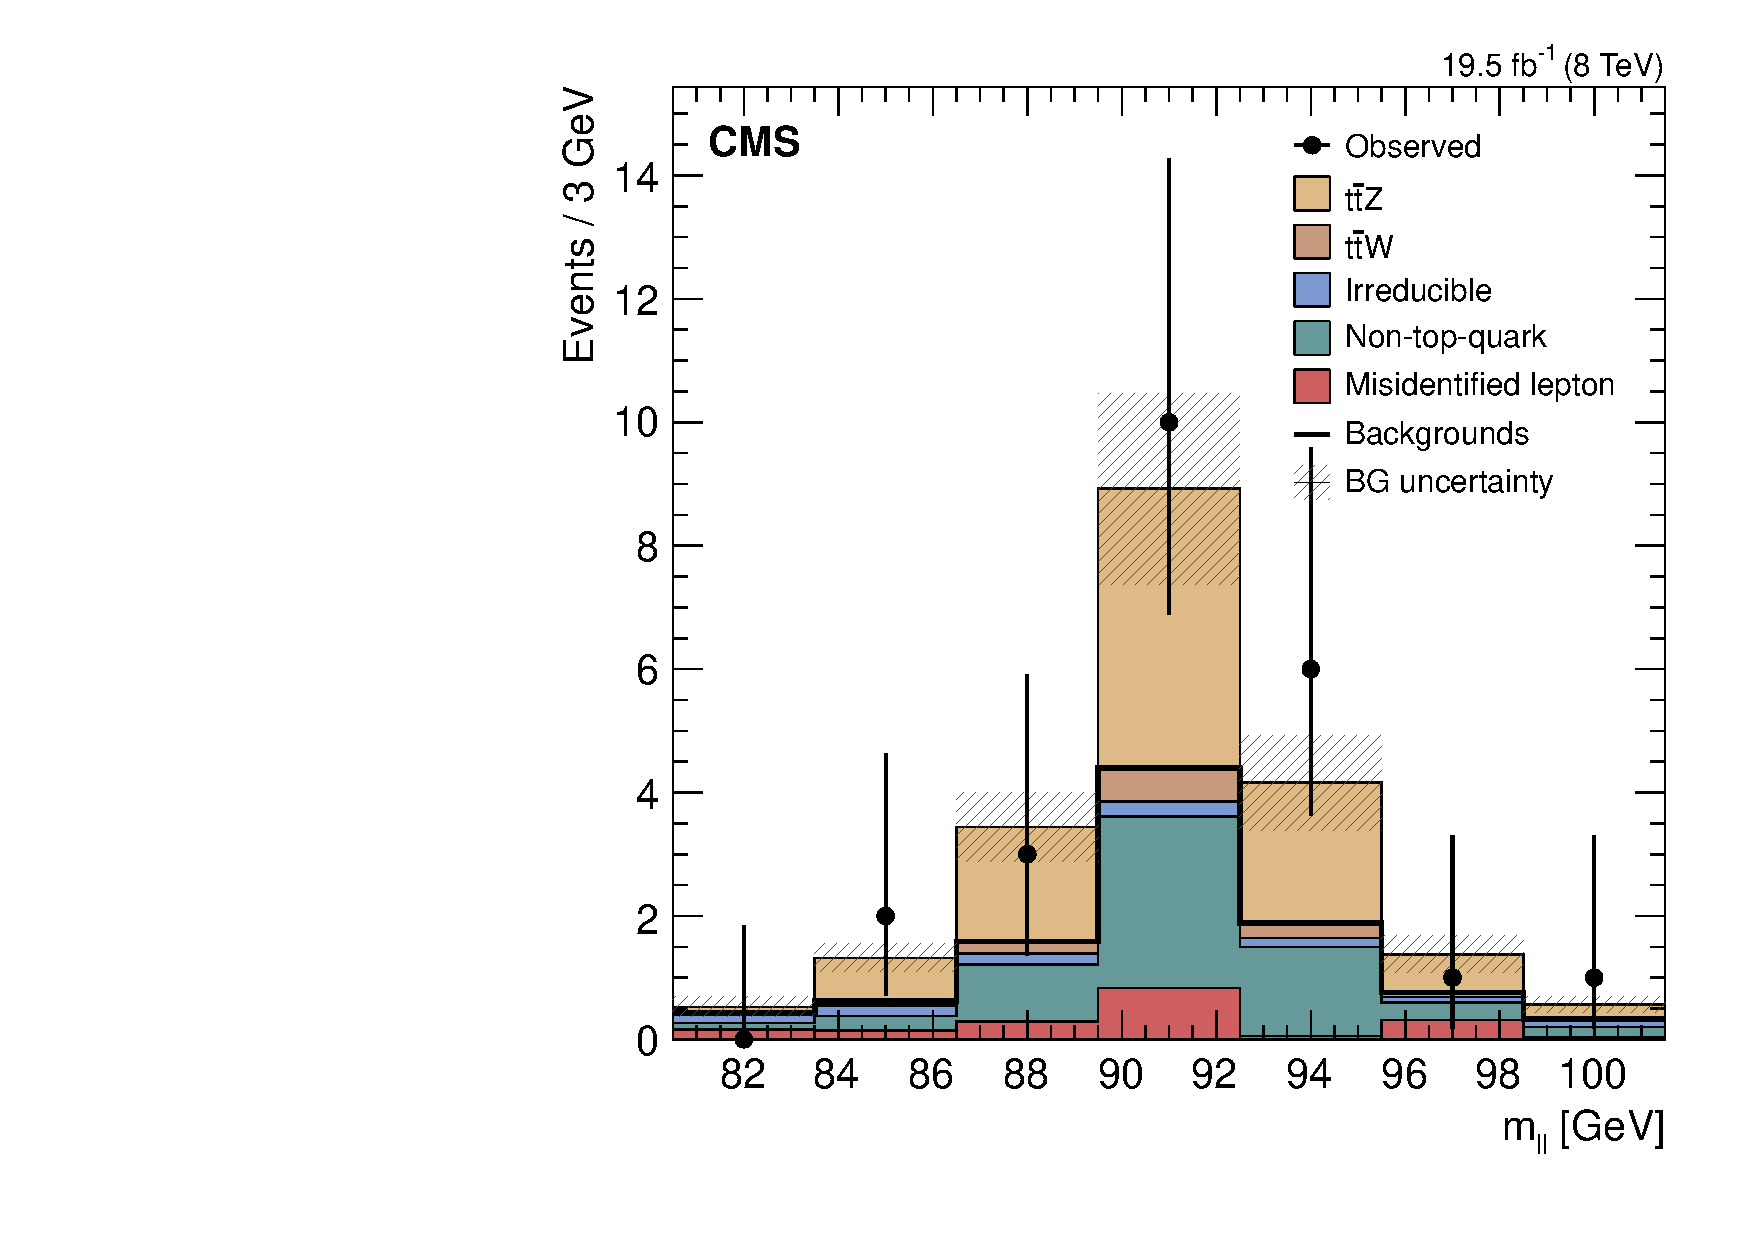
\includegraphics[width=0.48\linewidth]{Figs/Plots_PreSelections/hZMass_3L2b.pdf}
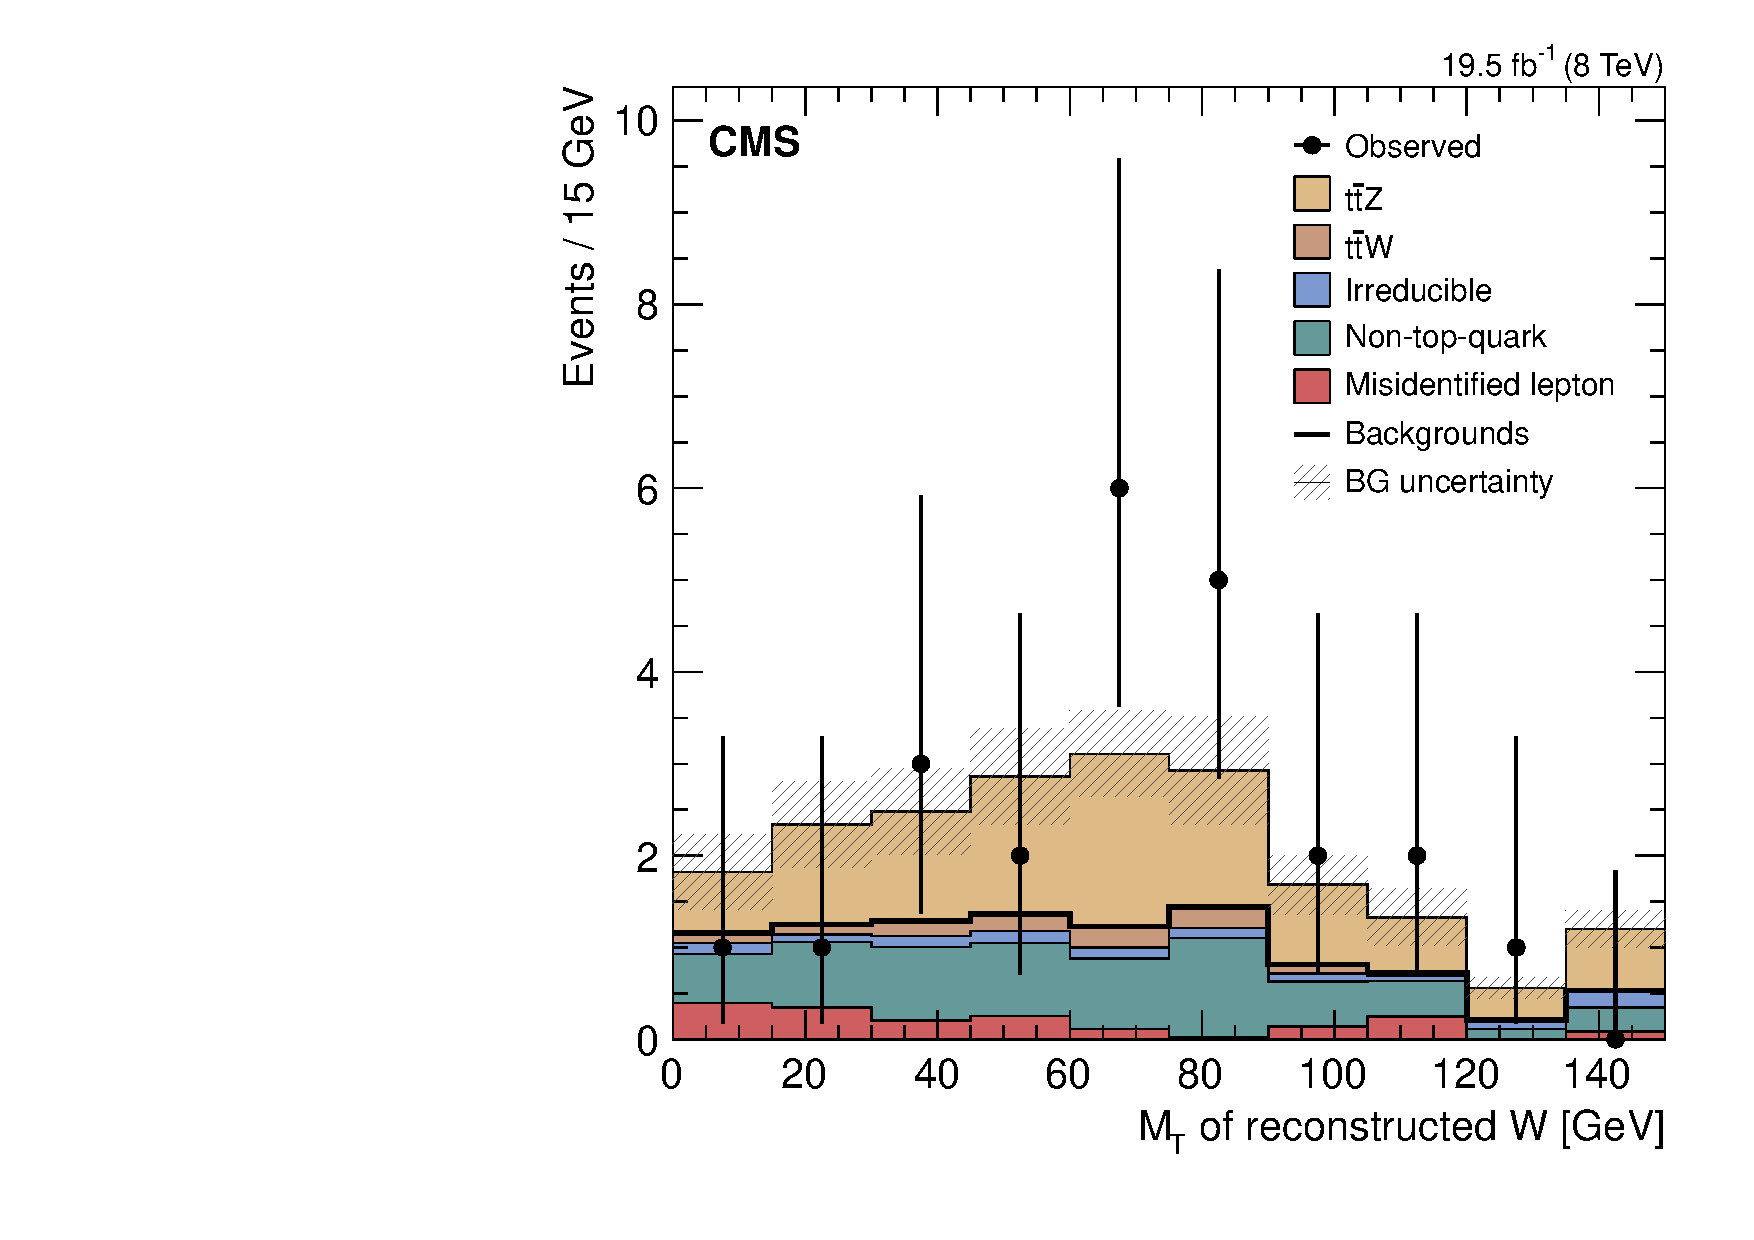
\includegraphics[width=0.48\linewidth]{Figs/Plots_PreSelections/hWMt_3L2b.pdf}
\caption{\label{fig:hmass_3L2b}
Reconstructed mass plots after tri-lepton plus two b-tag selections. Reconstructed Z Mass from lepton pair (Left). Reconstructed W \Mt \ (Right ).
}
\end{center}
\end{figure}



\begin{figure}[h]
\begin{center}
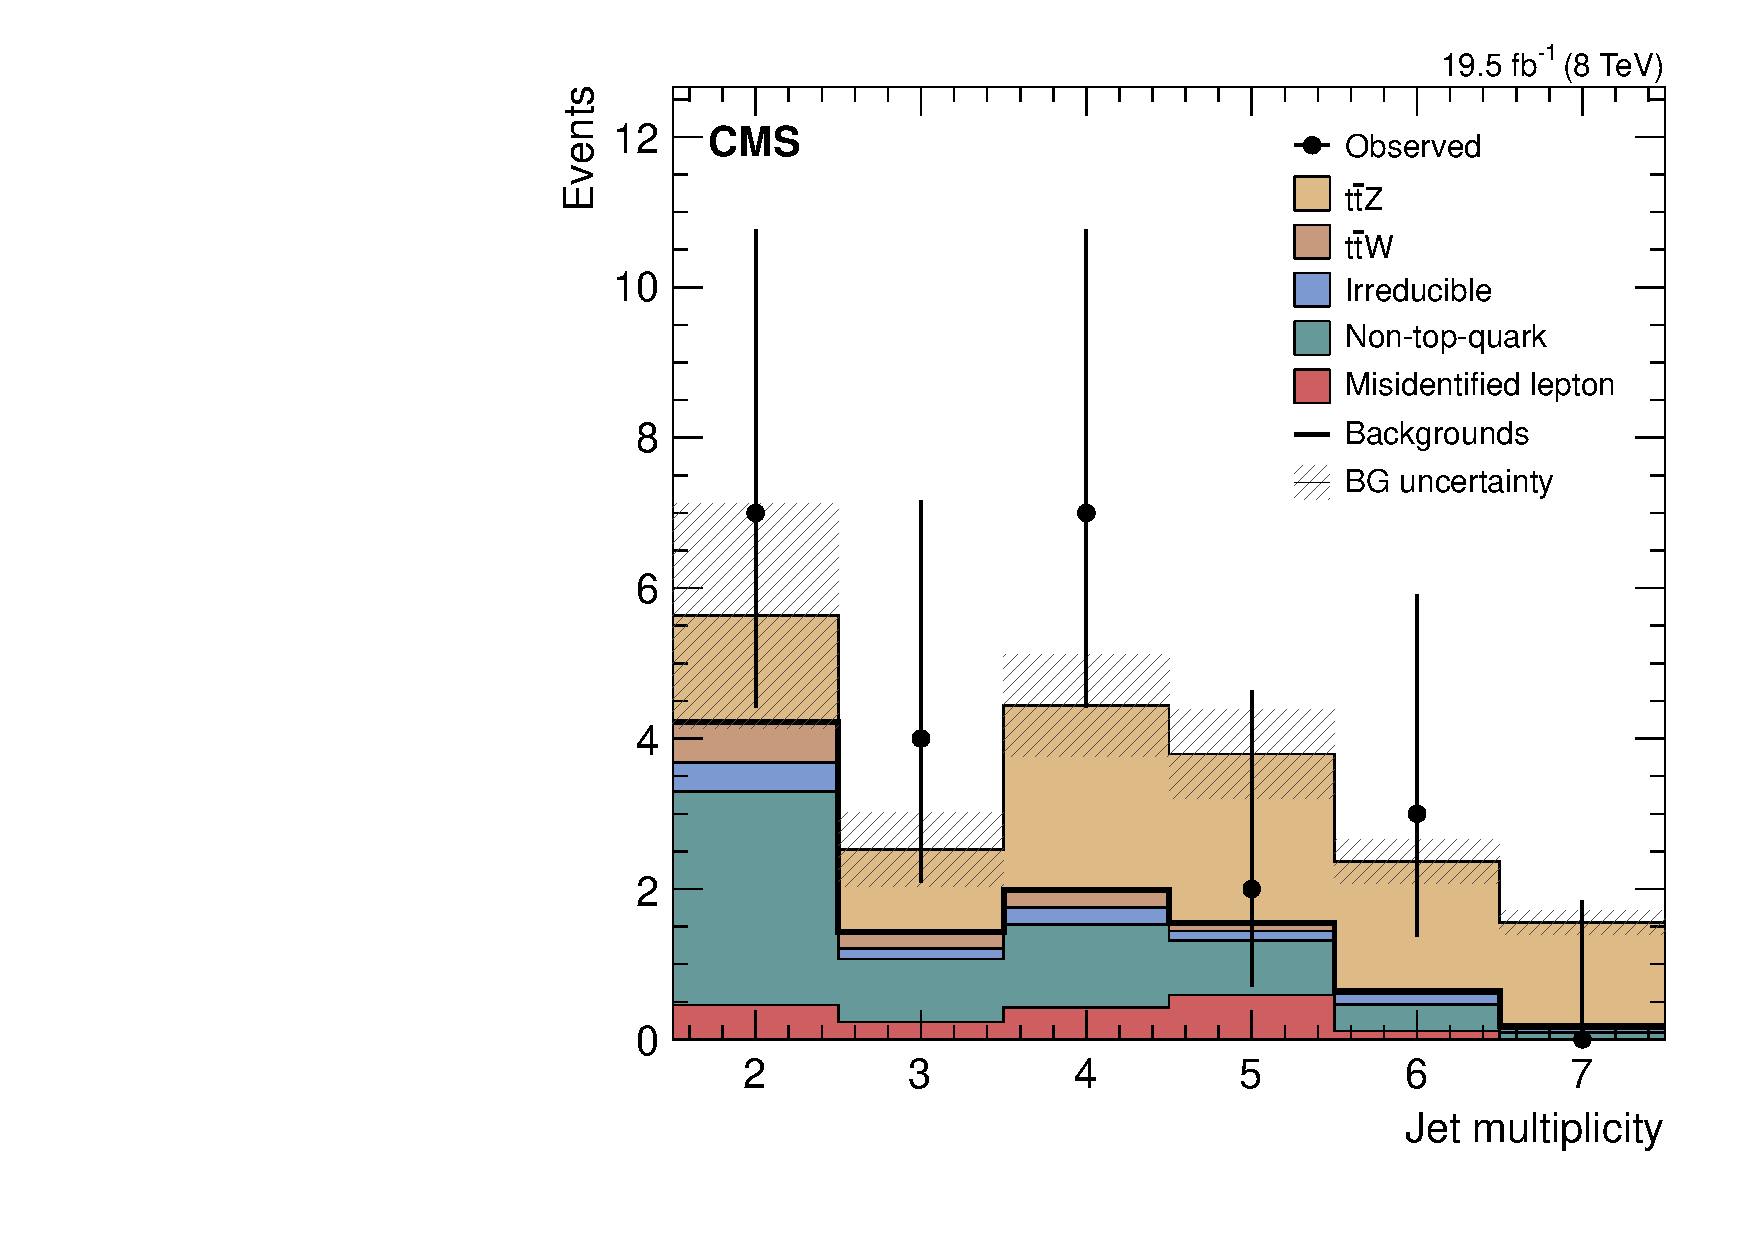
\includegraphics[width=0.48\linewidth]{Figs/Plots_PreSelections/hNJets_3L2b.pdf}
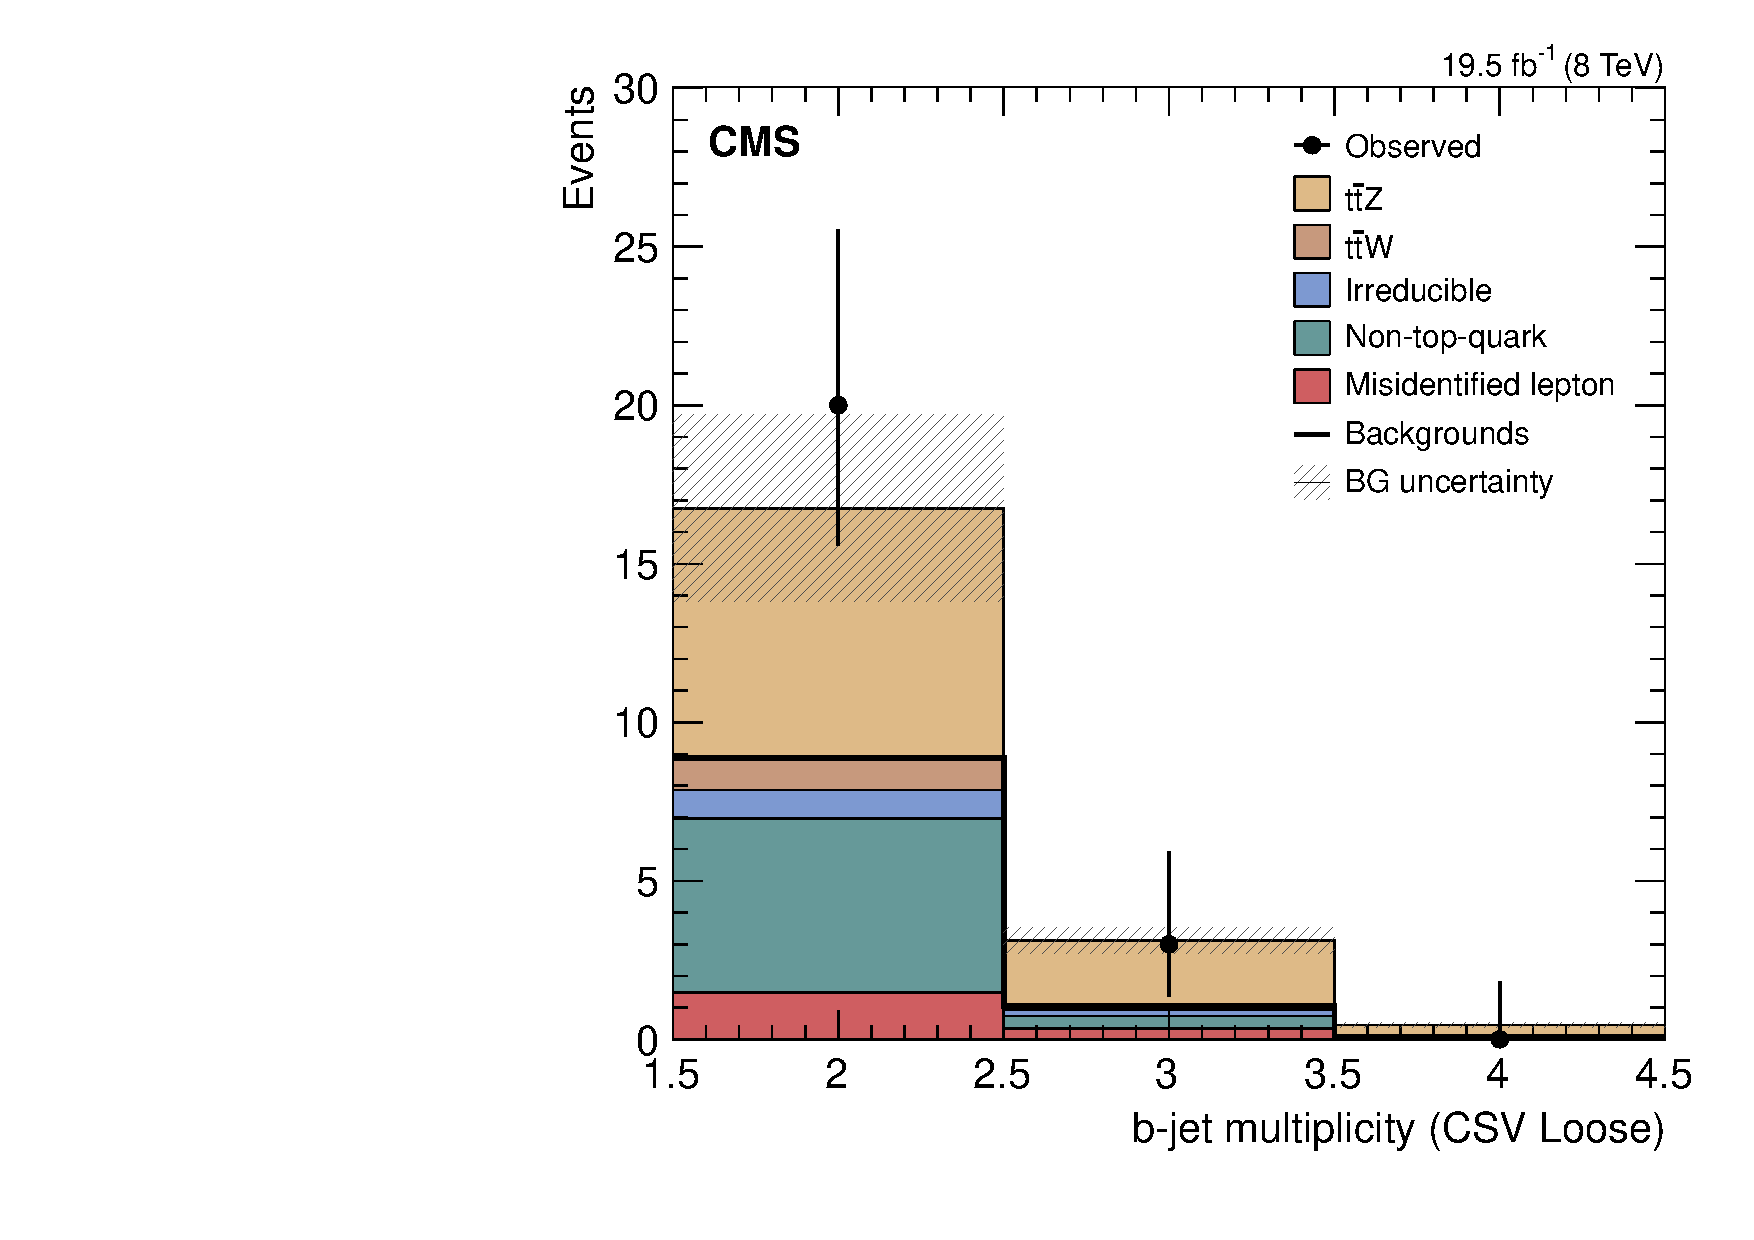
\includegraphics[width=0.48\linewidth]{Figs/Plots_PreSelections/hNLoose_3L2b.pdf}
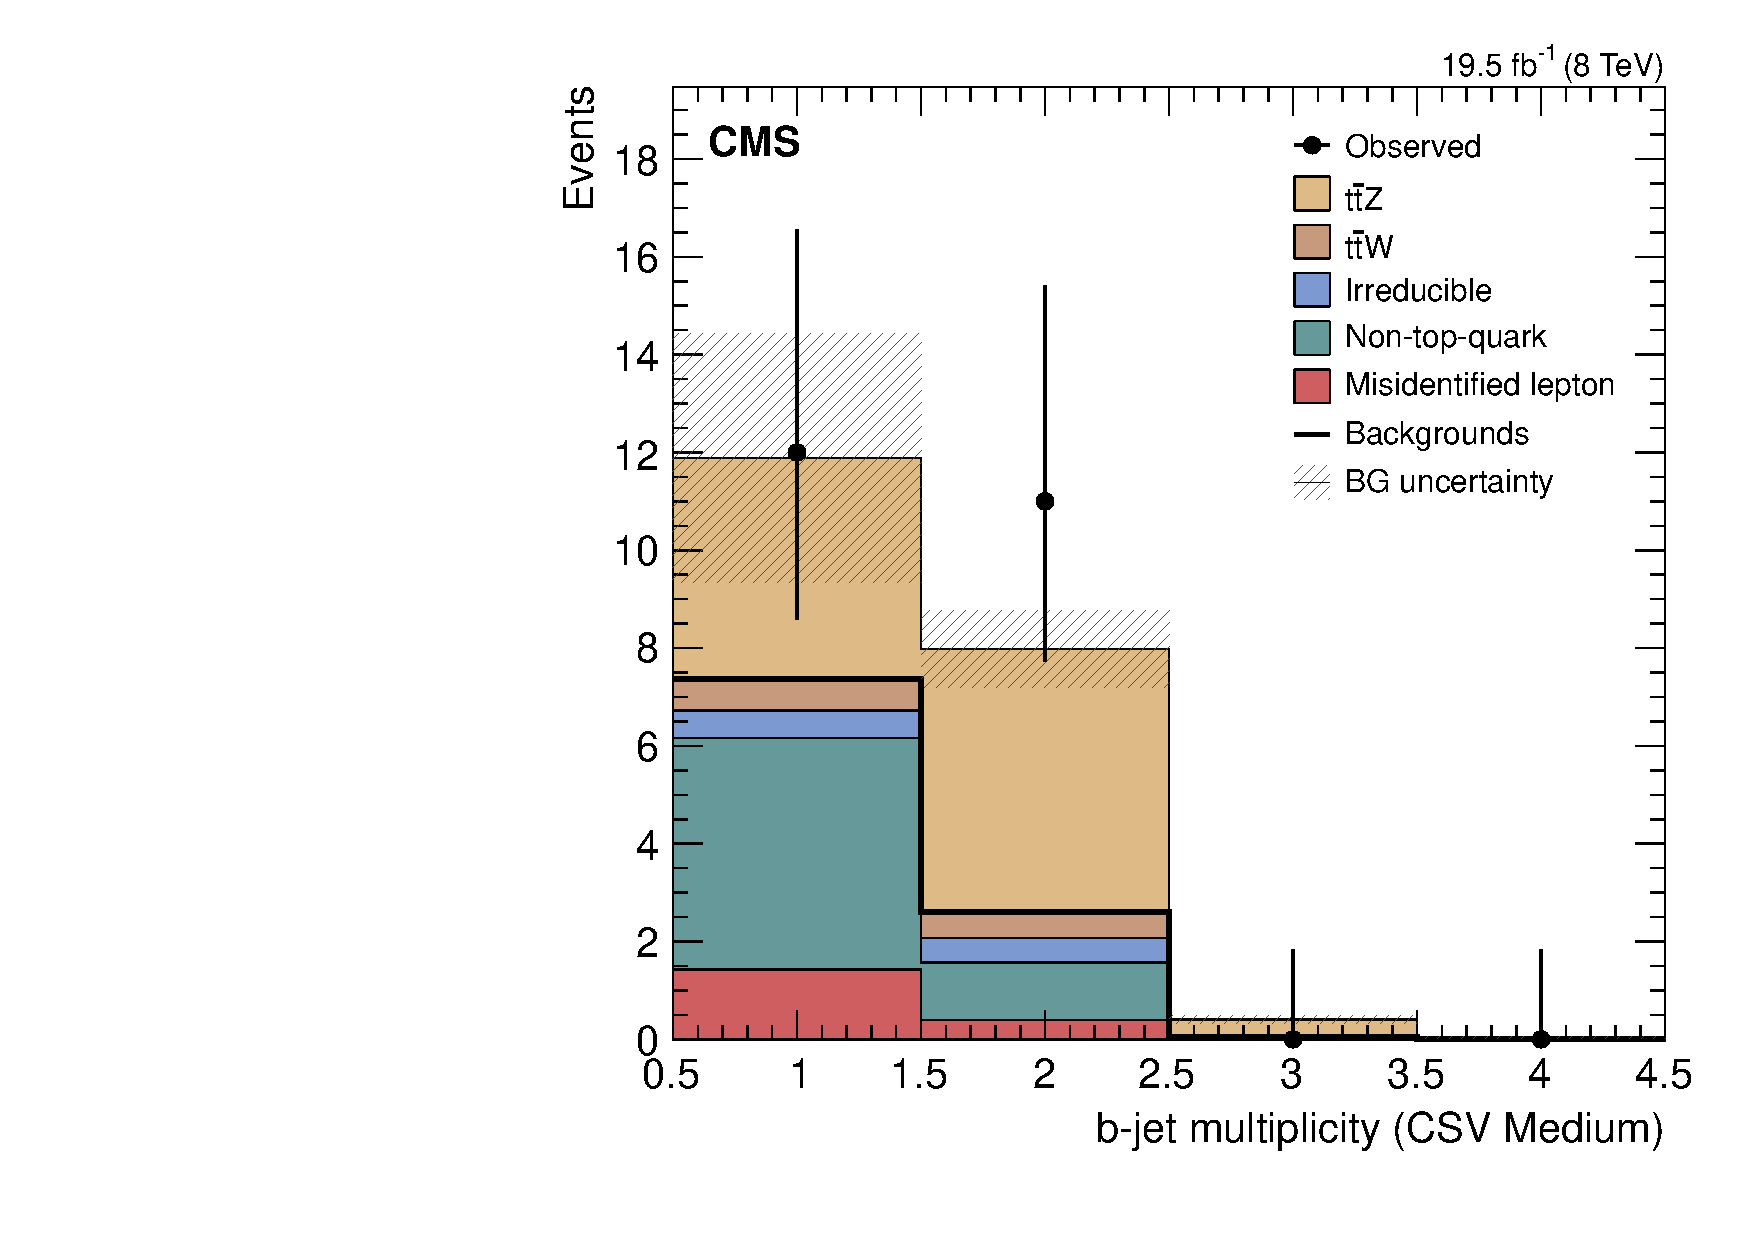
\includegraphics[width=0.48\linewidth]{Figs/Plots_PreSelections/hNMedium_3L2b.pdf}
\caption{\label{fig:jetmult_3L2b}
Jet Multiplicities. Left: Number of pfJets after tri-lepton plus two b-tag selections. Middle: Number of CSVL b-tags. Right: Number of CSVM b-tags.
}
\end{center}
\end{figure}



\begin{figure}[h]
\begin{center}
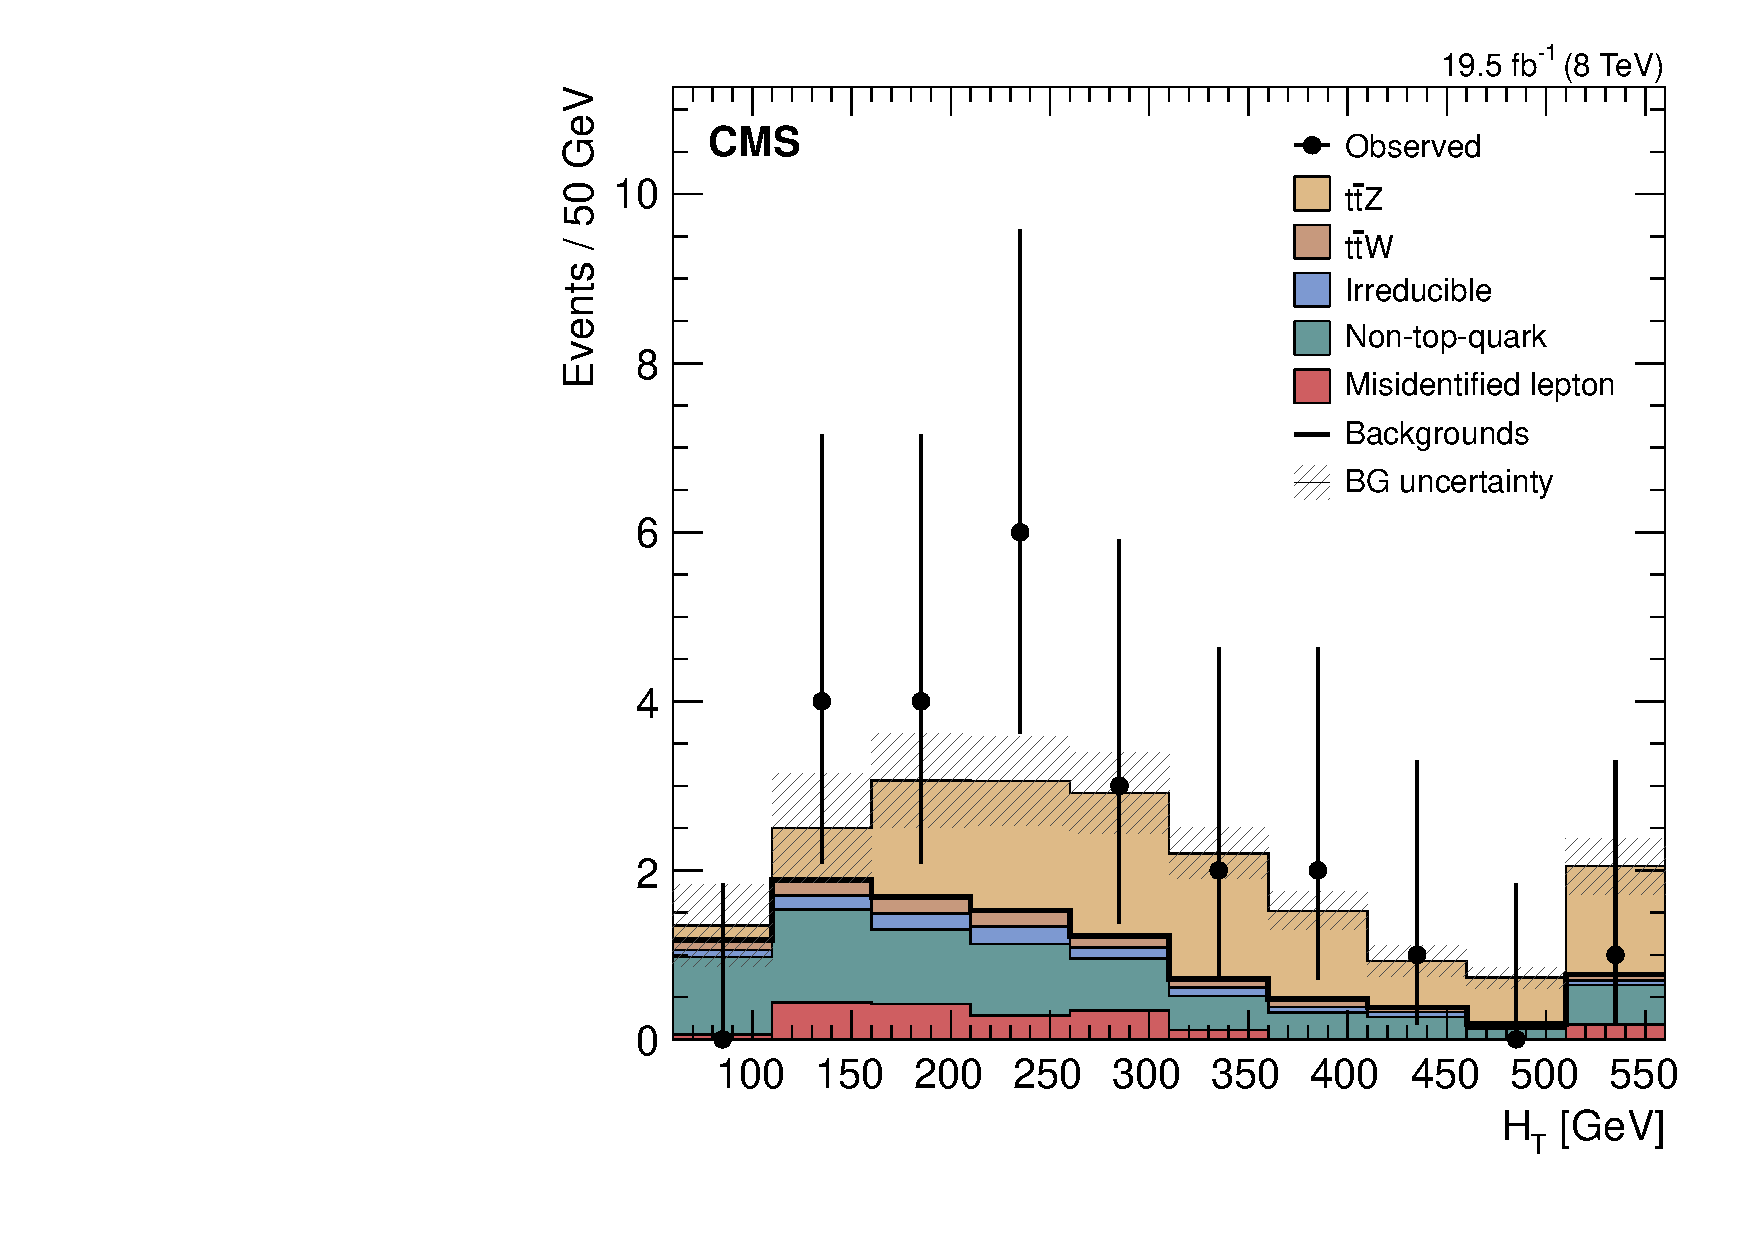
\includegraphics[width=0.48\linewidth]{Figs/Plots_PreSelections/hHt_3L2b.pdf}
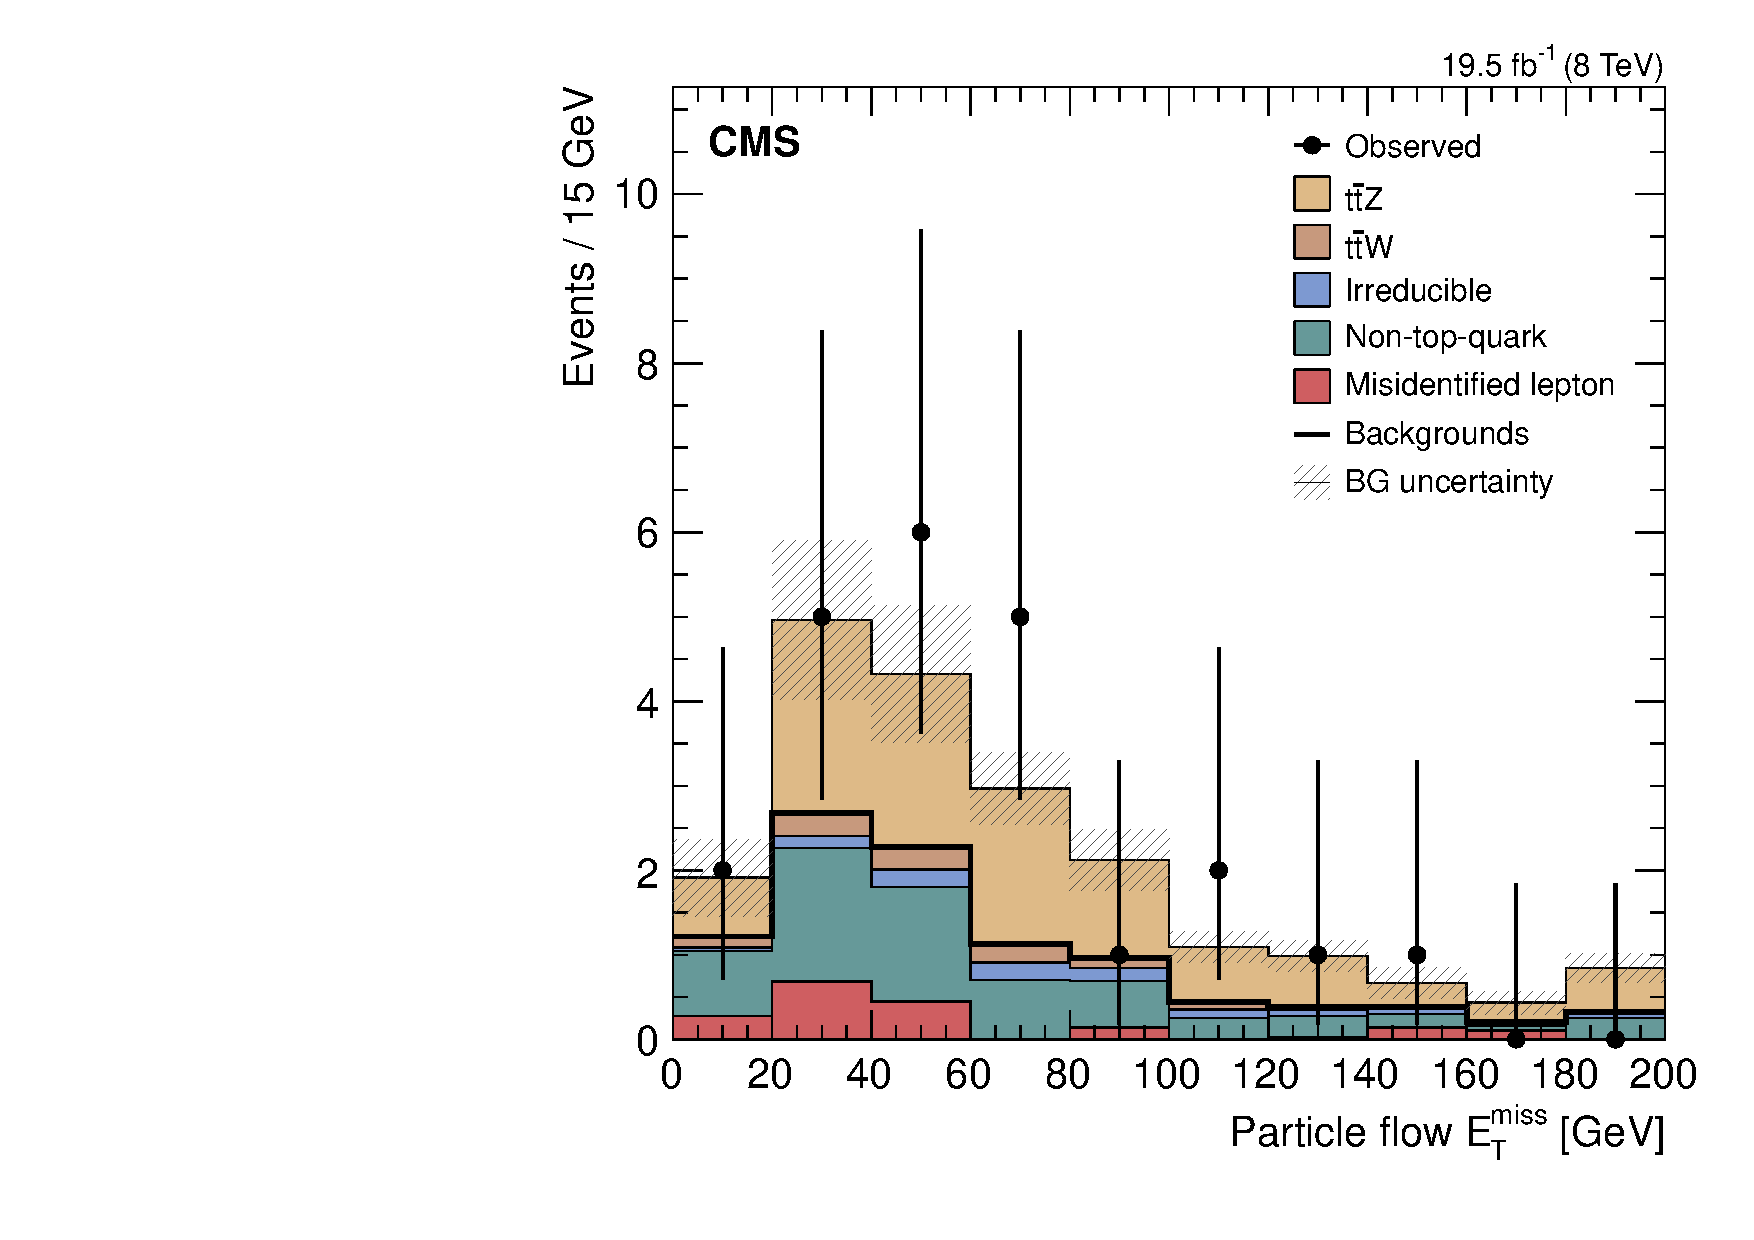
\includegraphics[width=0.48\linewidth]{Figs/Plots_PreSelections/hPFMet_3L2b.pdf}
\caption{\label{fig:hht_pfmet_3l}
Ht (Left) and pfMET(Right) after tri-lepton plus two b-tag selections. Agreement between measured data and predictions of signal and backgrounds are shown.
}
\end{center}
\end{figure}







         
	\section{Yields from Data After Full Selections}
	The yields in data and MC are summarized in Table~\ref{tab:yields} after applying the full analysis selections as listed in Sec~\ref{sec:EventSelections}. The MC is normalized to \intLumi of luminosity to match the data, and scaled by the lepton efficiency scale factors and b-tag discriminant re-weighting as described in Sections~\ref{sec:tag_and_probe} and~\ref{sec:btag_syst} respectively. The data yields are shown along side the MC yields to help demonstrate the relative contributions of the individual backgrounds. The data driven backgrounds were shown in a previous section and will be used in the next section to calculate the \ttZ \ signal. The irreducible backgrounds will be estimated from the yields in Table~\ref{tab:yields} using the line labeled $t\overline{t}$X/tbZ/VZZ. Given our lack of knowledge of cross sections for these processes and an inability to validate these MC samples against data, we assign a 50\% systematic.

\begin{sidewaystable}[ht!]
\caption{ \label{tab:yields} Data and pure MC yields after full analysis selections with \intLumi. Errors are statistical only. MC yields are shown to help understand the composition of the data yields.}
\begin{center}
\begin{tabular}{c|ccccc}\hline
&Yields (All)&Yields ($\mu\mu\mu$)&Yields ($\mu\mu$e)&Yields (ee$\mu$)&Yields (eee)\\
\hline \hline
W $\rightarrow \ell \nu$ & 0.00$\pm$0.89 & 0.00$\pm$0.89 & 0.00$\pm$0.89 & 0.00$\pm$0.89 & 0.00$\pm$0.89\\
VV $\rightarrow 2 \ell$ & 0.04$\pm$0.07 & 0.02$\pm$0.06 & 0.02$\pm$0.06 & 0.00$\pm$0.06 & 0.00$\pm$0.06\\
$t\overline{t}$ & 0.32$\pm$0.12 & 0.11$\pm$0.08 & 0.14$\pm$0.10 & 0.04$\pm$0.09 & 0.03$\pm$0.09\\
DY $\rightarrow 2 \ell$  & 0.00$\pm$0.60 & 0.00$\pm$0.60 & 0.00$\pm$0.60 & 0.00$\pm$0.60 & 0.00$\pm$0.60\\
VZ $\rightarrow 3\ell$ or $4\ell$ & 1.02$\pm$0.09 & 0.25$\pm$0.04 & 0.34$\pm$0.05 & 0.19$\pm$0.04 & 0.23$\pm$0.04\\
WWV & 0.13$\pm$0.03 & 0.03$\pm$0.01 & 0.02$\pm$0.01 & 0.05$\pm$0.02 & 0.03$\pm$0.01\\
\ttX/tbZ/VZZ & 0.98$\pm$0.08 & 0.32$\pm$0.05 & 0.20$\pm$0.04 & 0.24$\pm$0.05 & 0.22$\pm$0.04\\
\ttZ & 8.15$\pm$0.38 & 2.45$\pm$0.21 & 2.09$\pm$0.19 & 1.99$\pm$0.19 & 1.62$\pm$0.17\\
\hline \hline
Total Bkg MC (19.5 fb$^{-1}$) & 2.49$\pm$1.09 & 0.74$\pm$1.08 & 0.72$\pm$1.08 & 0.51$\pm$1.08 & 0.52$\pm$1.08\\
\hline
Total Sig+Bkg MC (19.5 fb$^{-1}$) & 10.64$\pm$1.15 & 3.19$\pm$1.10 & 2.81$\pm$1.10 & 2.50$\pm$1.10 & 2.14$\pm$1.09\\
\hline
Data (19.5 fb$^{-1}$) & 12.$\pm$3.46 & 3.$\pm$1.73 & 2.$\pm$1.41 & 4.$\pm$2.00 & 3.$\pm$1.73\\
\hline
\end{tabular}
\end{center}
\end{sidewaystable}

\clearpage

	\section{Measured Signal and Background Subtraction}
	\label{sec:signal}
Compiling the information in the preceding sections, an estimate can be made for the \ttZ \ signal in the measured data. The contribution due to di-lepton final states that pass the selection due to an additional ``fake" lepton in the event is described in Sec~\ref{sec:fake_estimation} and the contribution from tri-lepton events that pass the selection due to b-tagged jets that arise from gluon radiation is described in Sec~\ref{sec:brate_estimation}. Finally, the irreducible backgrounds which cannot be estimated by a data driven method are taken from the row labeled ``\ttX/tbZ/VZZ" in Table~\ref{tab:yields} where the ``X" is short hand for W, $\gamma$, or WW. Table~\ref{tab:signal_minus_bkg} summarizes the full yields in data after selections as well as the background estimates. Additionally a final estimate for the \ttZ \ to three lepton signal is shown.

\begin{table}[ht!]
\caption{ \label{tab:signal_minus_bkg} Data and pure MC yields after full analysis selections with \intLumi. Predictions for each background contribution are shown.}
\begin{center}
\begin{tabular}{c|c}\hline
 & Measurement\\
\hline \hline
Data (19.5 fb $^{-1}$)                         & $12. $ \\
%\hdashline
Bkg from Non-Prompt Leptons                   &  $- 1.13 \pm 0.51_{st} \pm 0.57_{sy}$ \\
Bkg from b-tags From Radiation                &  $- 2.27 \pm 0.51_{st} \pm 1.14_{sy}$ \\
Bkg from Irreducible                          &  $- 0.98 \pm 0.08_{st} \pm 0.49_{sy}$ \\
%\hdashline
Total Background Prediction                   &  $-4.38 \pm 0.73_{bkg st} \pm 1.37_{bkg sy}$ \\
\hline
Predicted Signal                              &  $7.62 \pm 3.46_{data st} \pm 0.73_{bkg st} \pm 1.37_{bkg sy}$ \\	
\hline
\end{tabular}
\end{center}
\end{table}



	
	\subsection{Method for Reconstructing a Top Mass}
	The selections chosen allow the identification of all of the constituent components of the top which decays to final state quarks. A good test for the accuracy and purity of the selection is to recreate a top mass. Determining which  particles actually came from the top is difficult. With more total events in the final selection to choose from, a more complicated but somewhat accurate algorithm could be chosen. With the lower number of events passing the selections in this document, a simple algorithm must be chosen to identify the jets from the hadronic top. There are few events, the algorithm must choose jets for each one, yet be simple enough not to sculpt the distribution. We following steps are taken:
\begin{enumerate}
\item Choose three jets, one of which has a CSVL or better b-tag that minimizes three jet system $\Delta R$ defined as
\begin{equation}
\Delta R_{j1,j2,b1} = \sqrt{ \left(\Delta R_{j1, ``top"} \right) ^2 + \left(\Delta R_{j2, ``top"} \right) ^2 + \left(\Delta R_{b1, ``top"} \right) ^2 }
\end{equation}
where ``top'' is the composite object created by summing the 4-vectors of the three jets.
\item Choose the highest pt b-jet out of the remaining b-tagged jets that are not part of the three jet system in step 1. This b-jet is considered to be from the leptonic top.
\end{enumerate}

Fig~\ref{fig:htopmass_3l2j2b} shows the hadronic top mass, hadronic W mass, and invariant mass of the b-jet and lepton from the leptonic top (with the neutrino unaccounted for for obvious reasons).


\begin{figure}[h]
\begin{center}
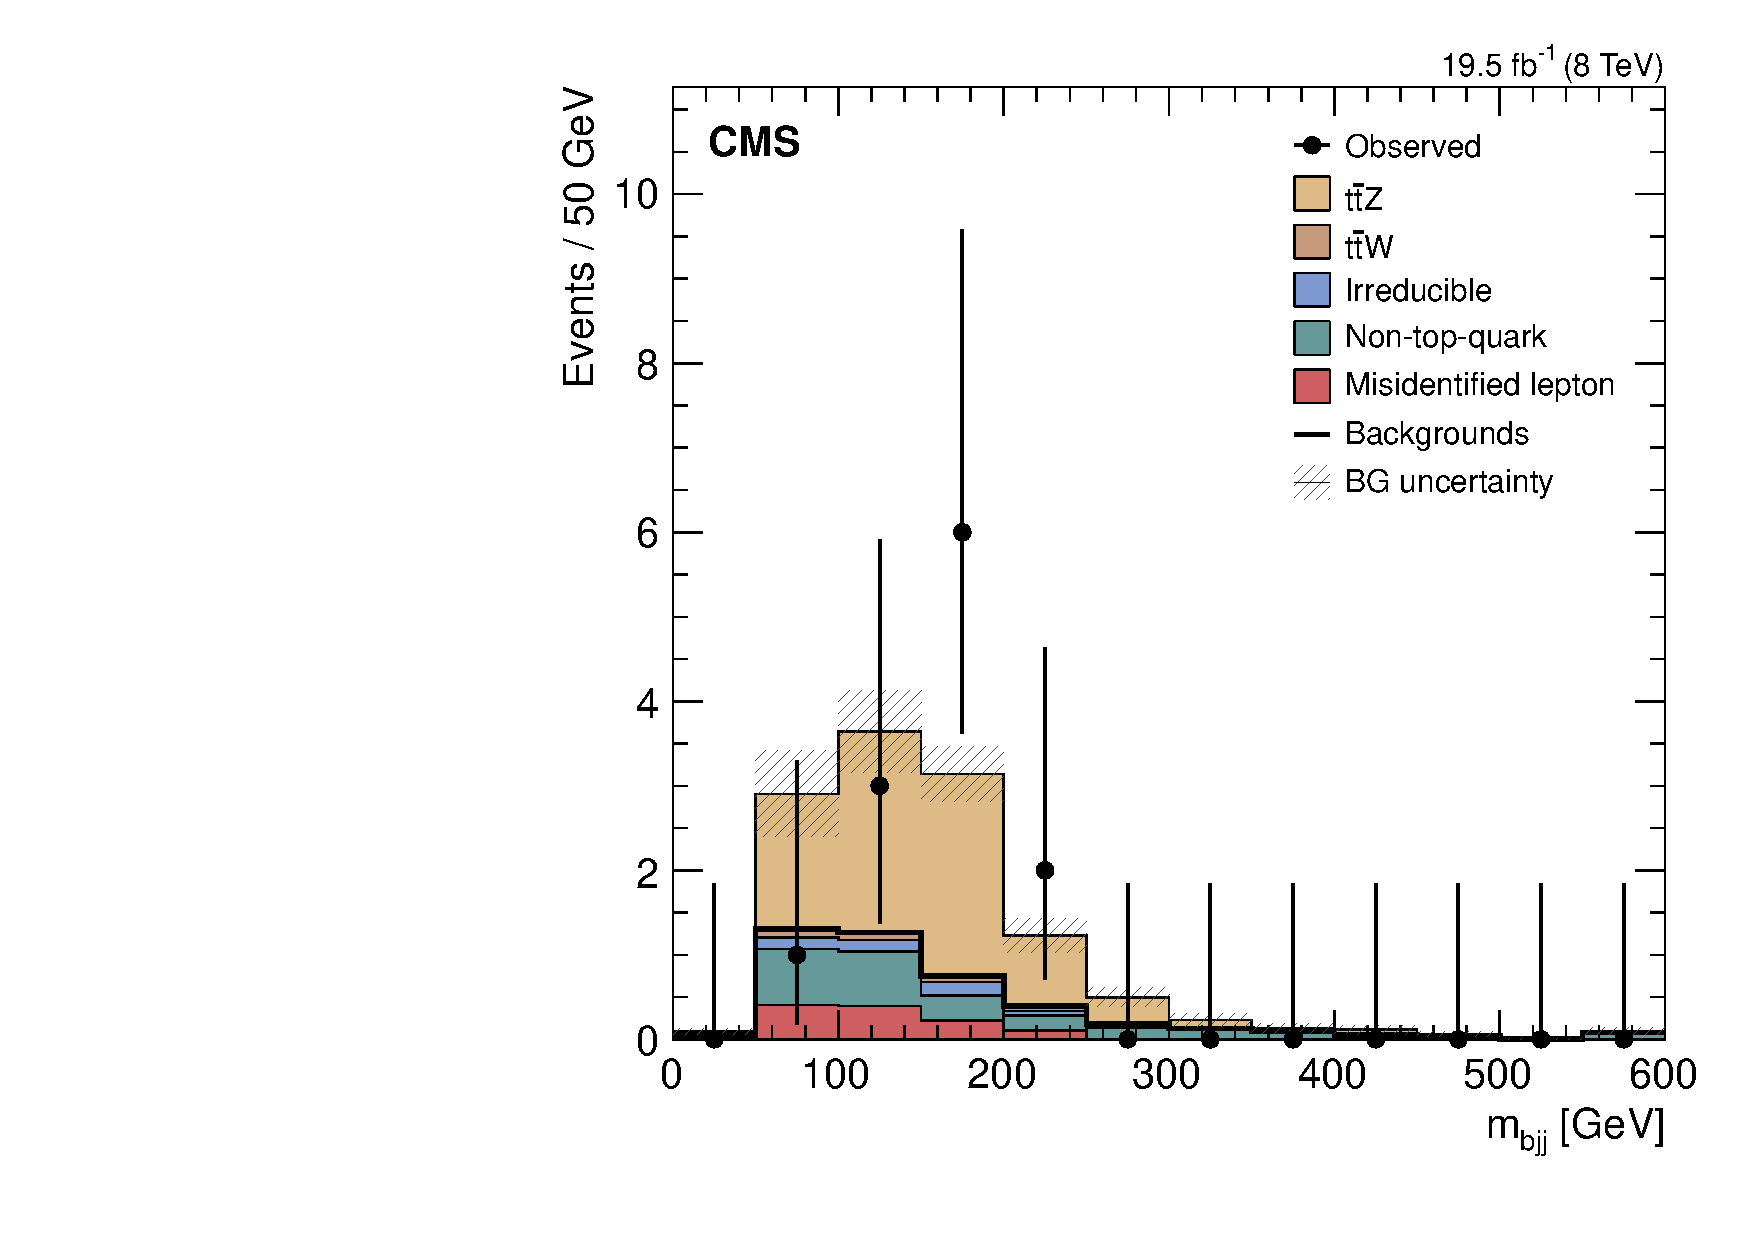
\includegraphics[width=0.48\linewidth]{Figs/Plots_Final_Selections/hTopMass_3L2J2b.pdf}
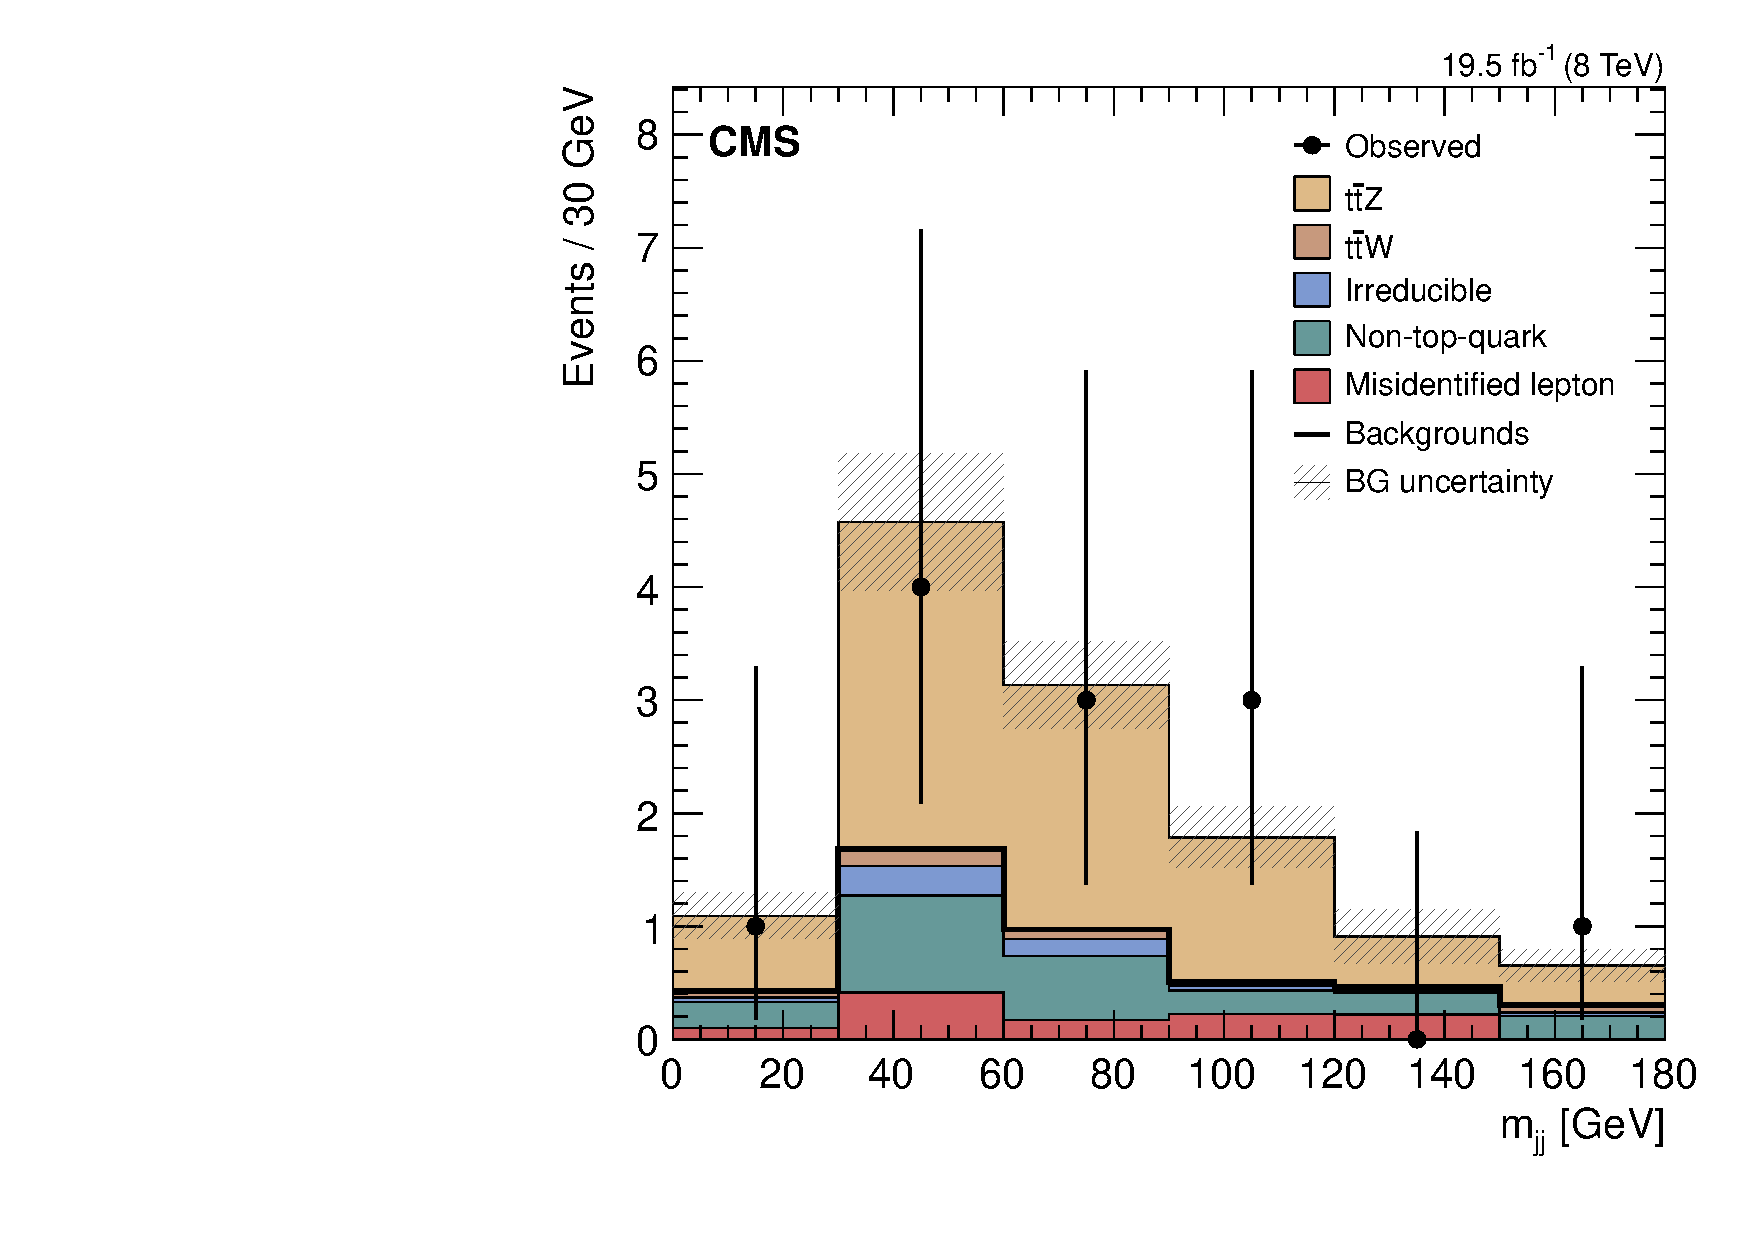
\includegraphics[width=0.48\linewidth]{Figs/Plots_Final_Selections/hTopWMass_3L2J2b.pdf}
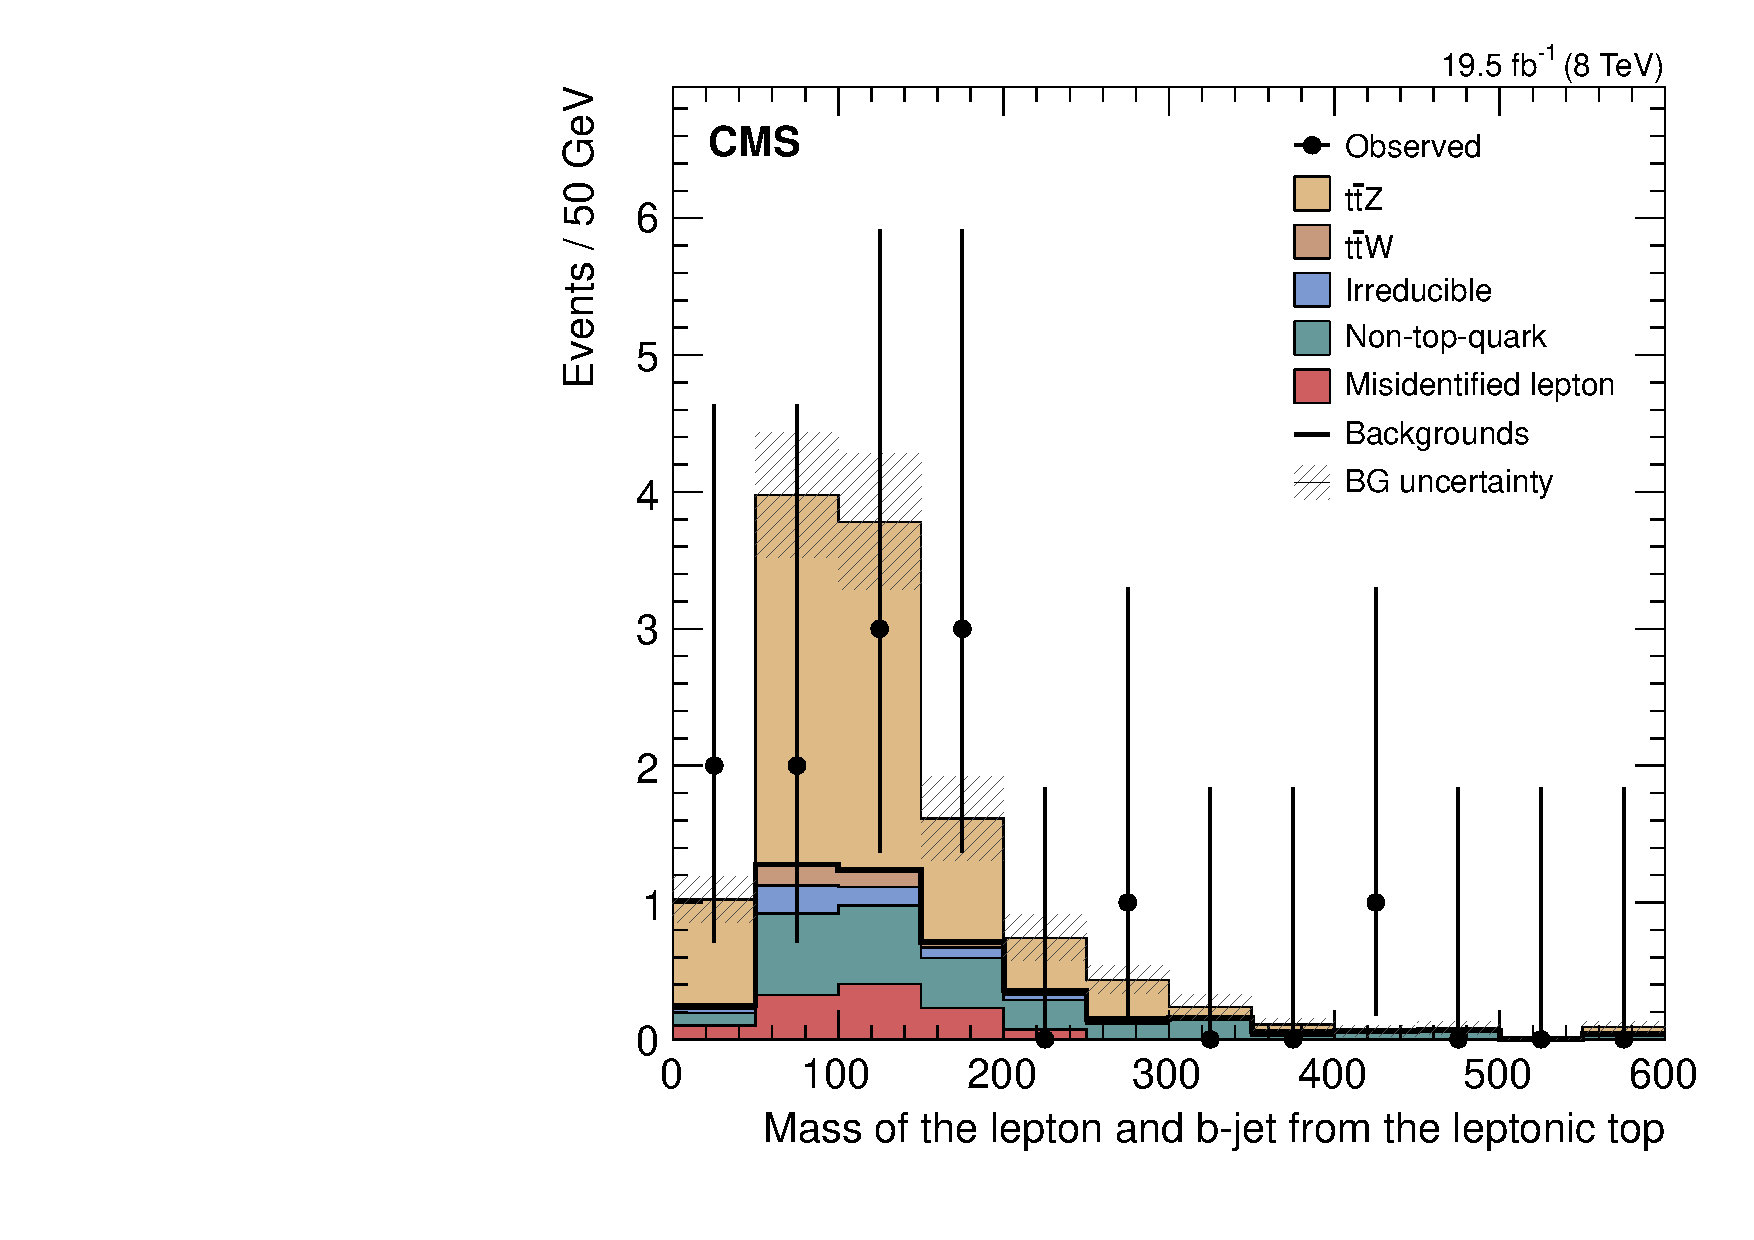
\includegraphics[width=0.48\linewidth]{Figs/Plots_Final_Selections/hTopbLMass_3L2J2b.pdf}
\caption{\label{fig:htopmass_3l2j2b}
Reconstructed mass of the hadronic top is shown after all selections have been applied (Top Left). Reconstructed mass of the hadronic W is shown after all selections have been applied(Top Right). Invariant mass of the W lepton with the b-jet from the leptonic top is shown (Bottom).
}
\end{center}
\end{figure}
	
	
	
	
	
	
	
	\subsection{Distributions with Full Selections}	
	
	The full analysis selection is described in Sec~\ref{sec:EventSelections}. This includes leptonic selections for reconstructing a Z from two leptons and requiring a third lepton that could be from a W. It also includes requiring four or more jets with two of them being b-tagged (one CSVL and one CSVM). After selection, the \ttZ \ contribution as predicted in MC is strong and the backgrounds have been reduced to a manageable level. In the following plots, data driven predictions are again used for normalization of backgrounds while MC is used for the shape (except in the case of the irreducible backgrounds where MC is used for shape and normalization). Although being lower in statistics, there is reasonable agreement between data and predictions (shape and size). Relevant plots are shown below. Fig~\ref{fig:hmass_3l2j2b} shows the reconstructed masses of the Z and the leptonic W (using \Mt) %while FIgure ~\ref{fig:htopmass_3l2j2b} shows the top (using the W \Mt \ for the W's contribution). 
These plots are used to demonstrate a degree of certainty that the correct events are being identified. %since the various underlying bosons and quarks can be reconstructed. \\

\begin{figure}[h]
\begin{center}
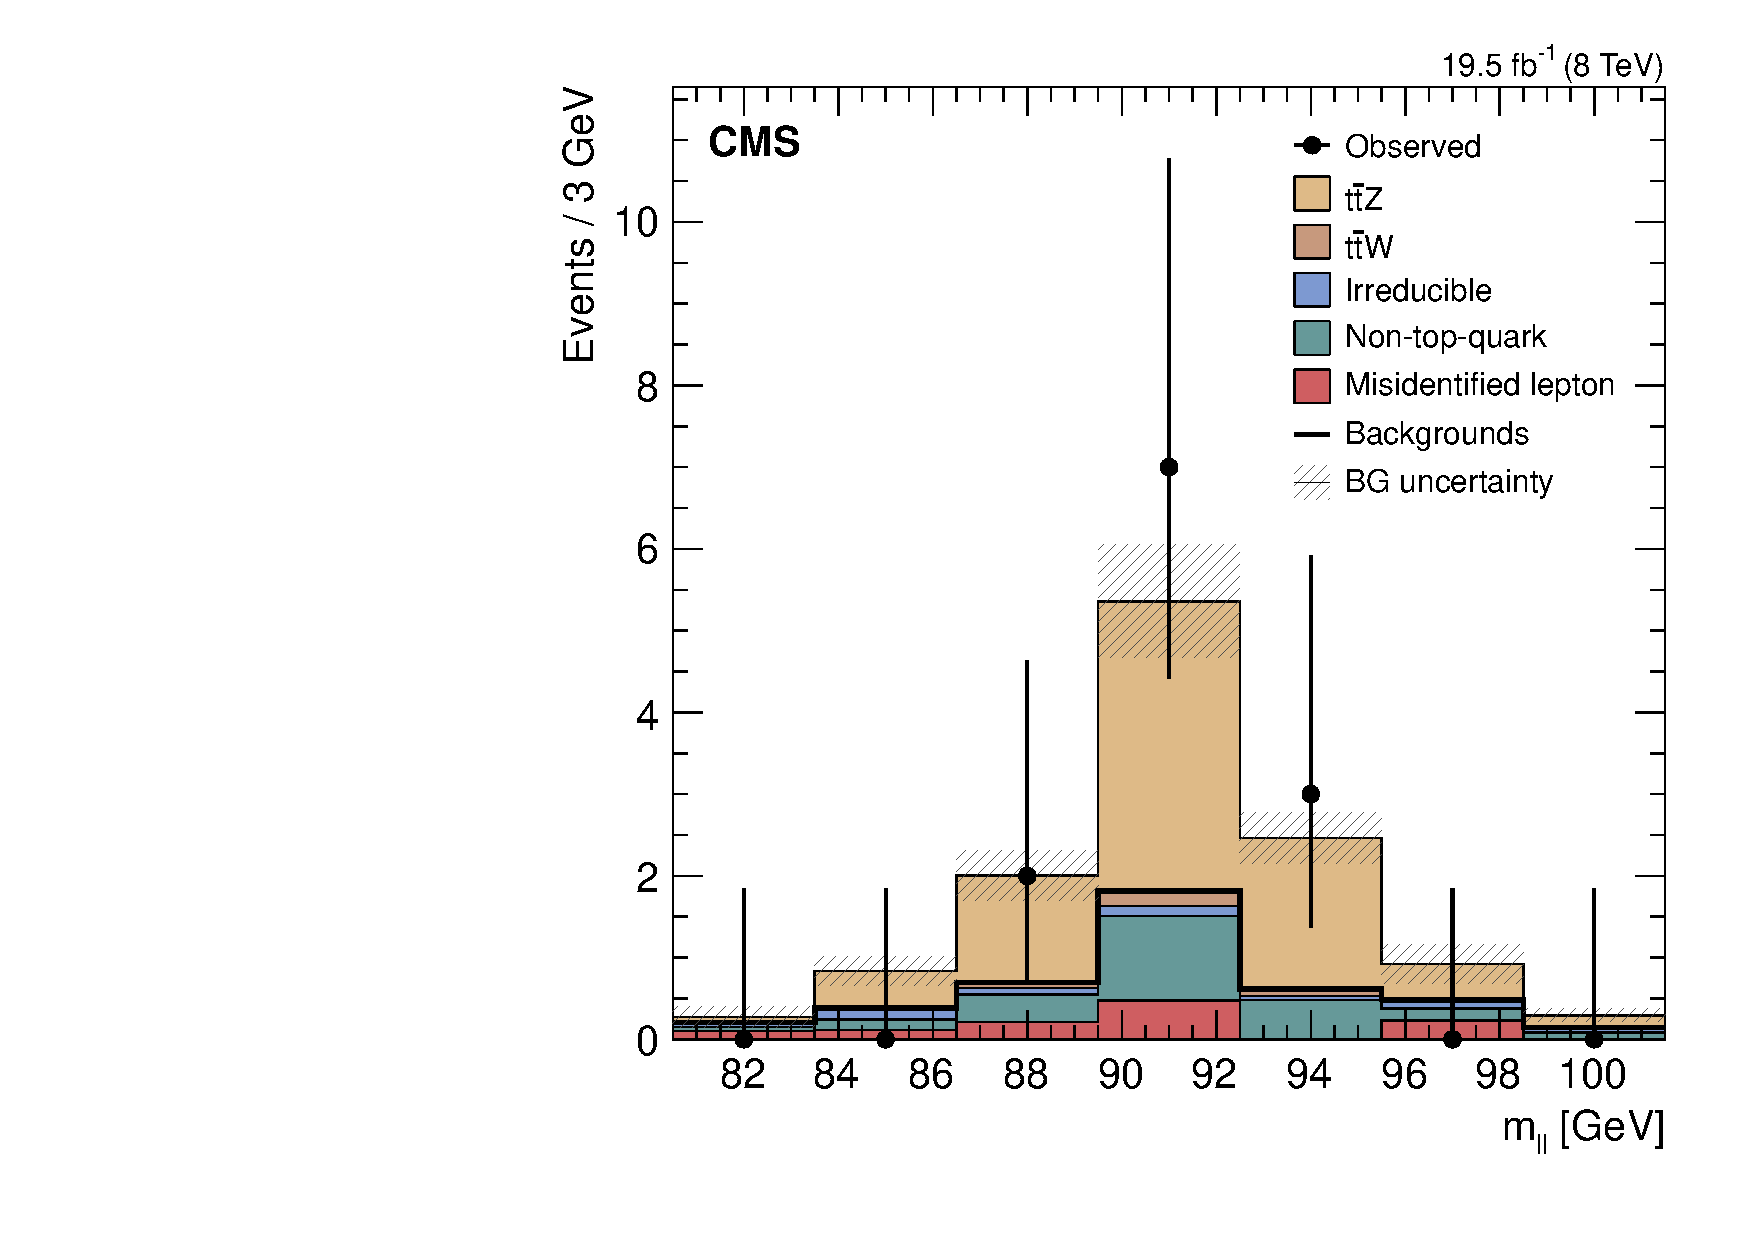
\includegraphics[width=0.48\linewidth]{Figs/Plots_Final_Selections/hZMass_3L2J2b.pdf}
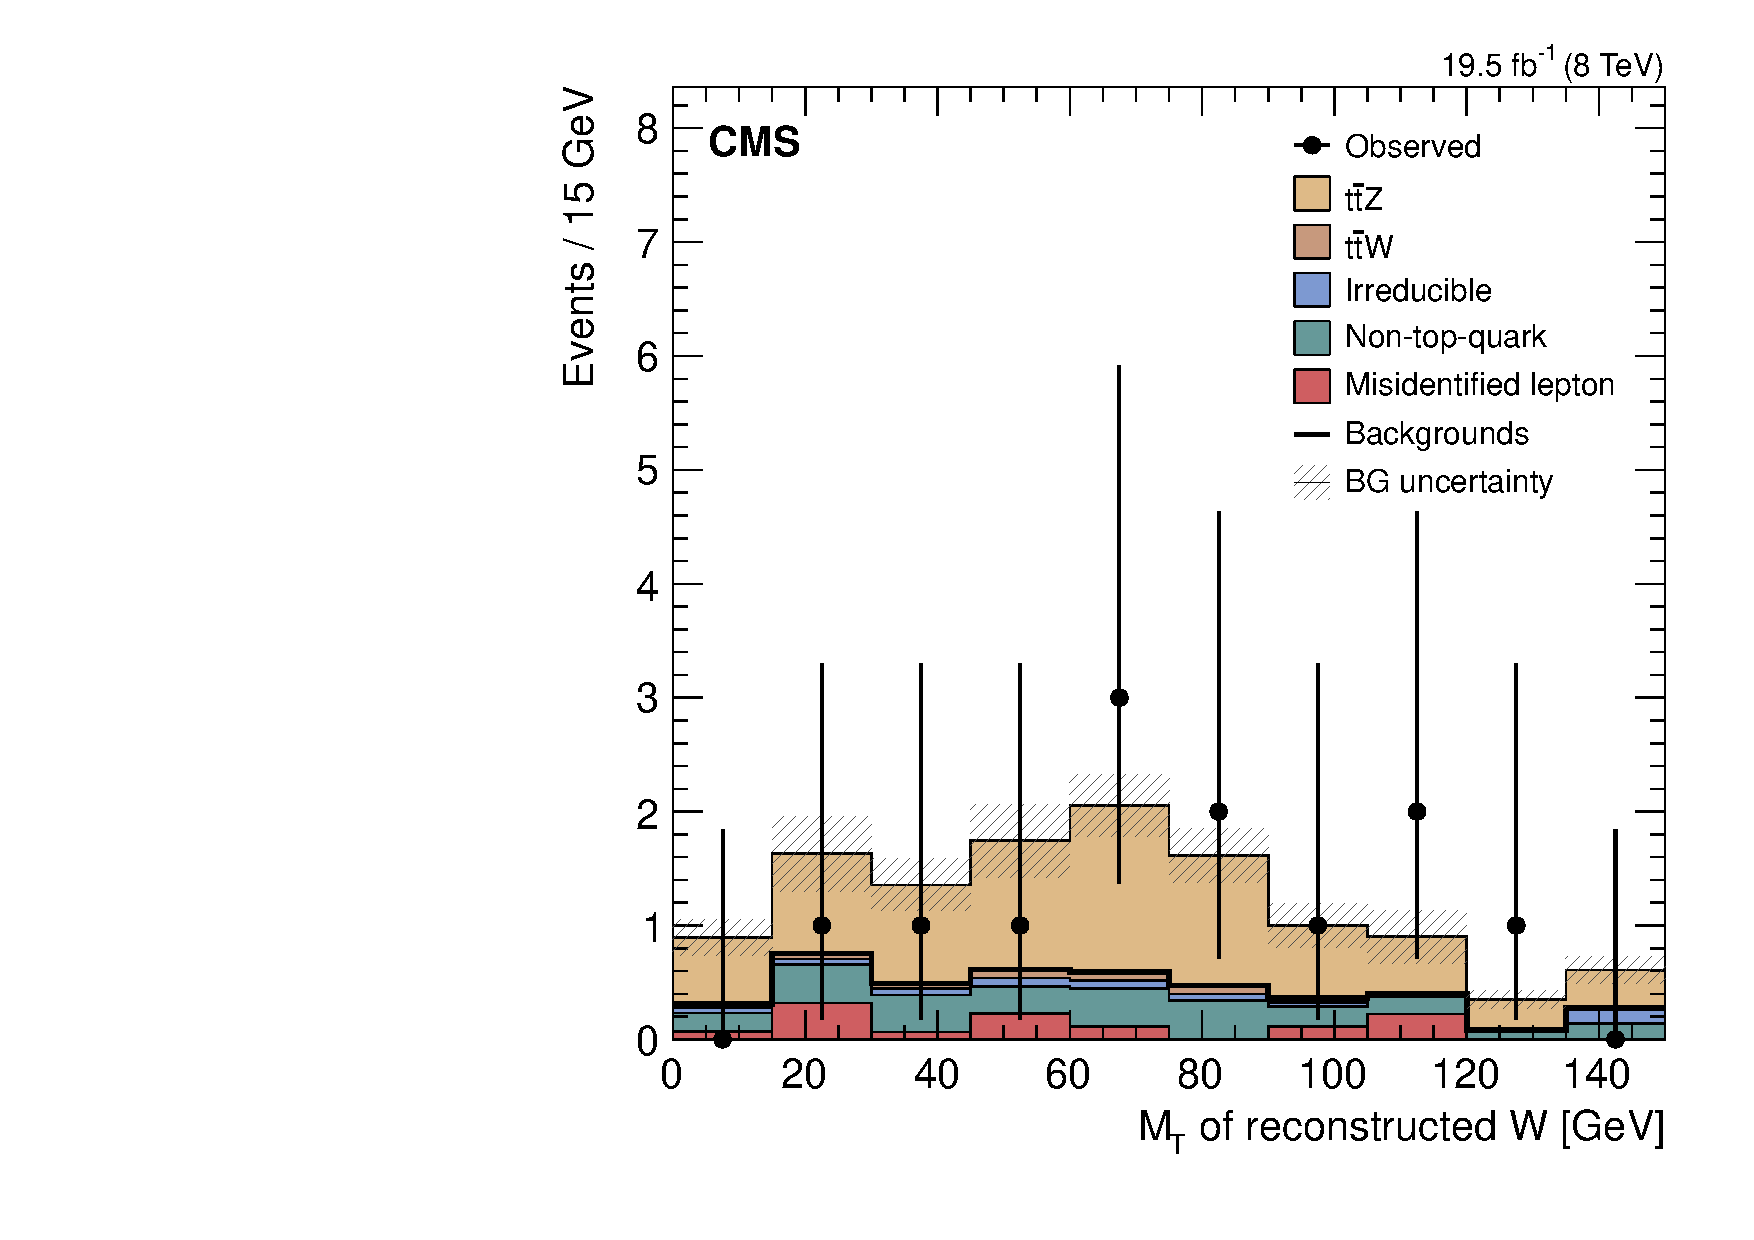
\includegraphics[width=0.48\linewidth]{Figs/Plots_Final_Selections/hWMt_3L2J2b.pdf}
\caption{\label{fig:hmass_3l2j2b}
Reconstructed mass of Z (Left) and \Mt of the W (Right) are shown after all selections have been applied.
}
\end{center}
\end{figure}


Figs~\ref{fig:hpfMET_3l2j2b} and~\ref{fig:hHt_3l2j2b} show two more defining characteristics. Both the pfMET and \HT \ are important shapes caused by the neutrino produced in the leptonic W decay and the jets produced in the top and hadronic W decay (respectively). Since these variables are not used in the current selections, they are plotted to show extra confirmation of the yields.

\begin{figure}[h]
\begin{center}
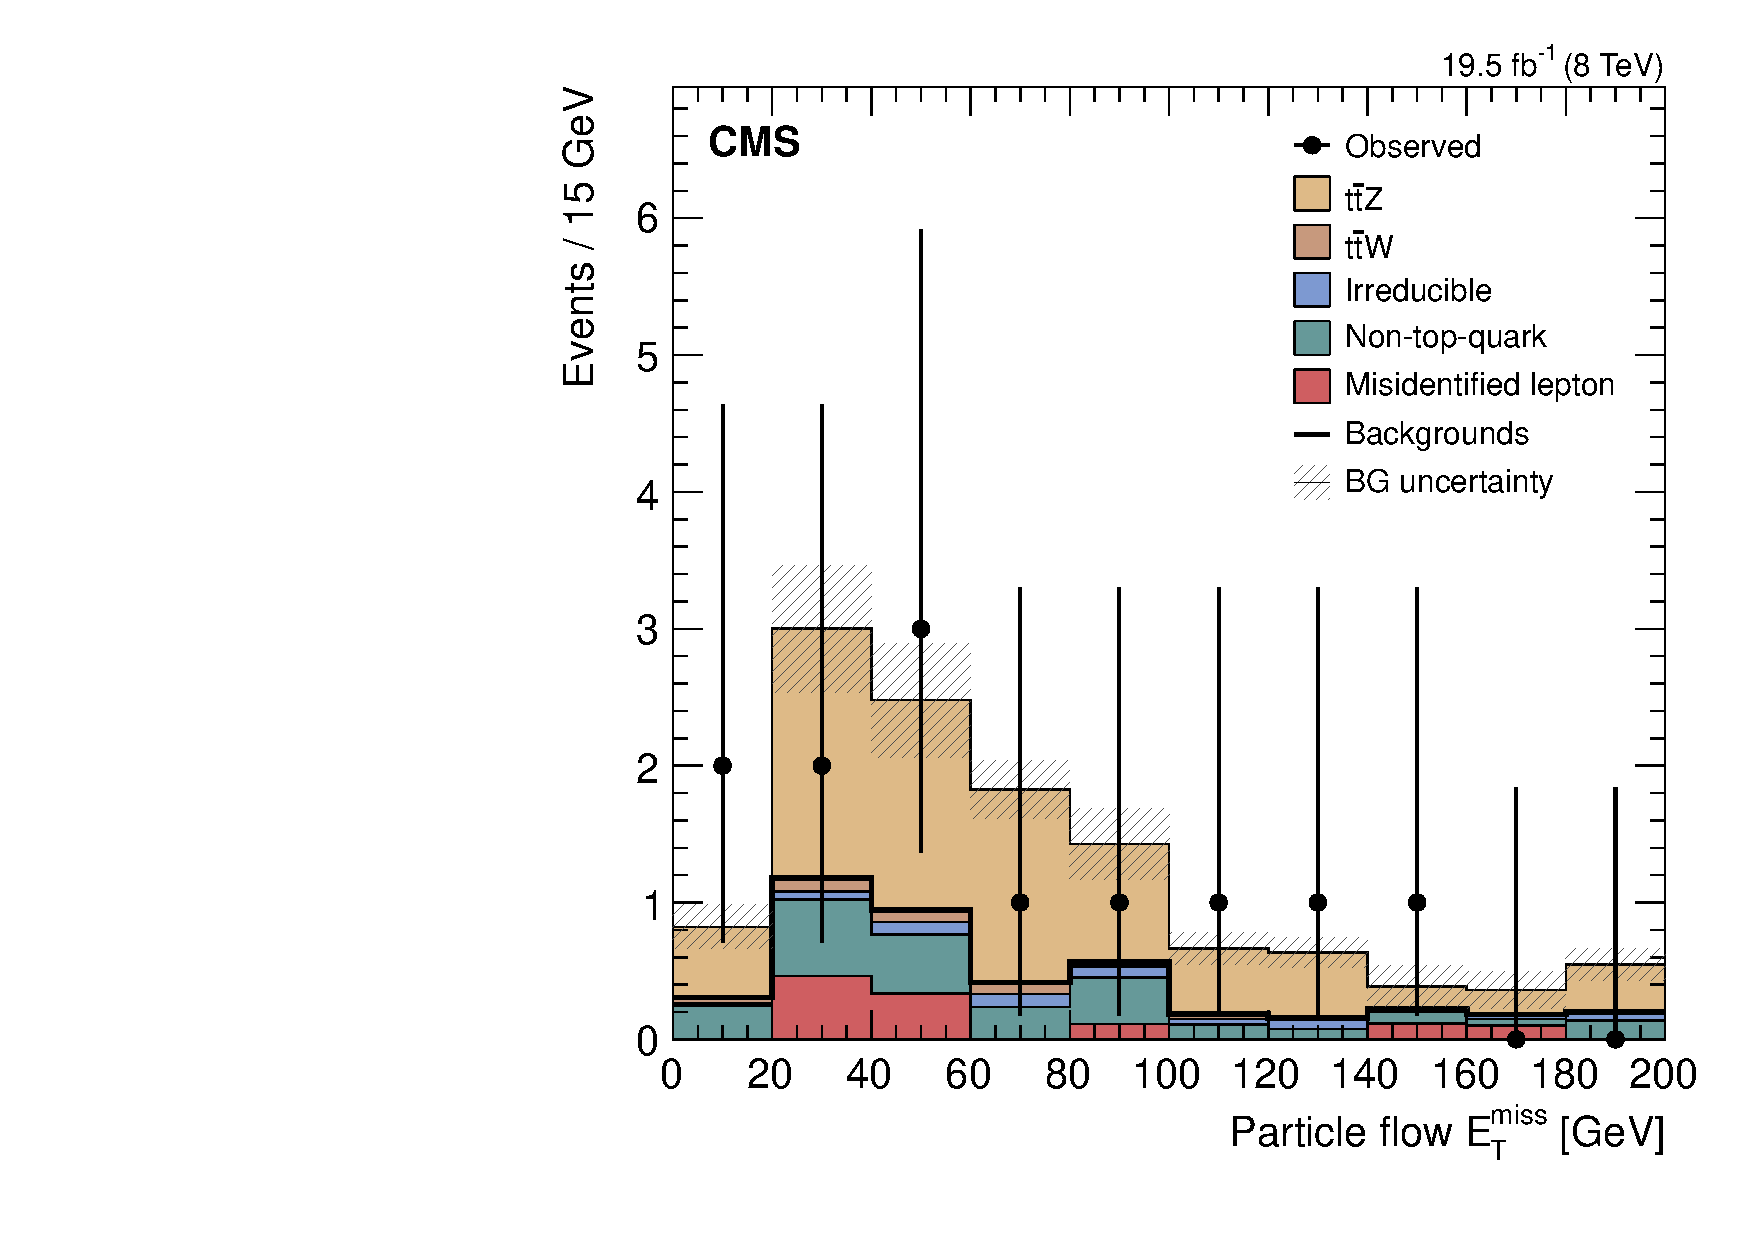
\includegraphics[width=0.6\linewidth]{Figs/Plots_Final_Selections/hpfMET_3L2J2b.pdf}
\caption{\label{fig:hpfMET_3l2j2b}
pfMET of the events after full analysis selections have been applied. This shows general agreement between measured data and predicted signal and backgrounds. 
}
\end{center}
\end{figure} 

\begin{figure}[h]
\begin{center}
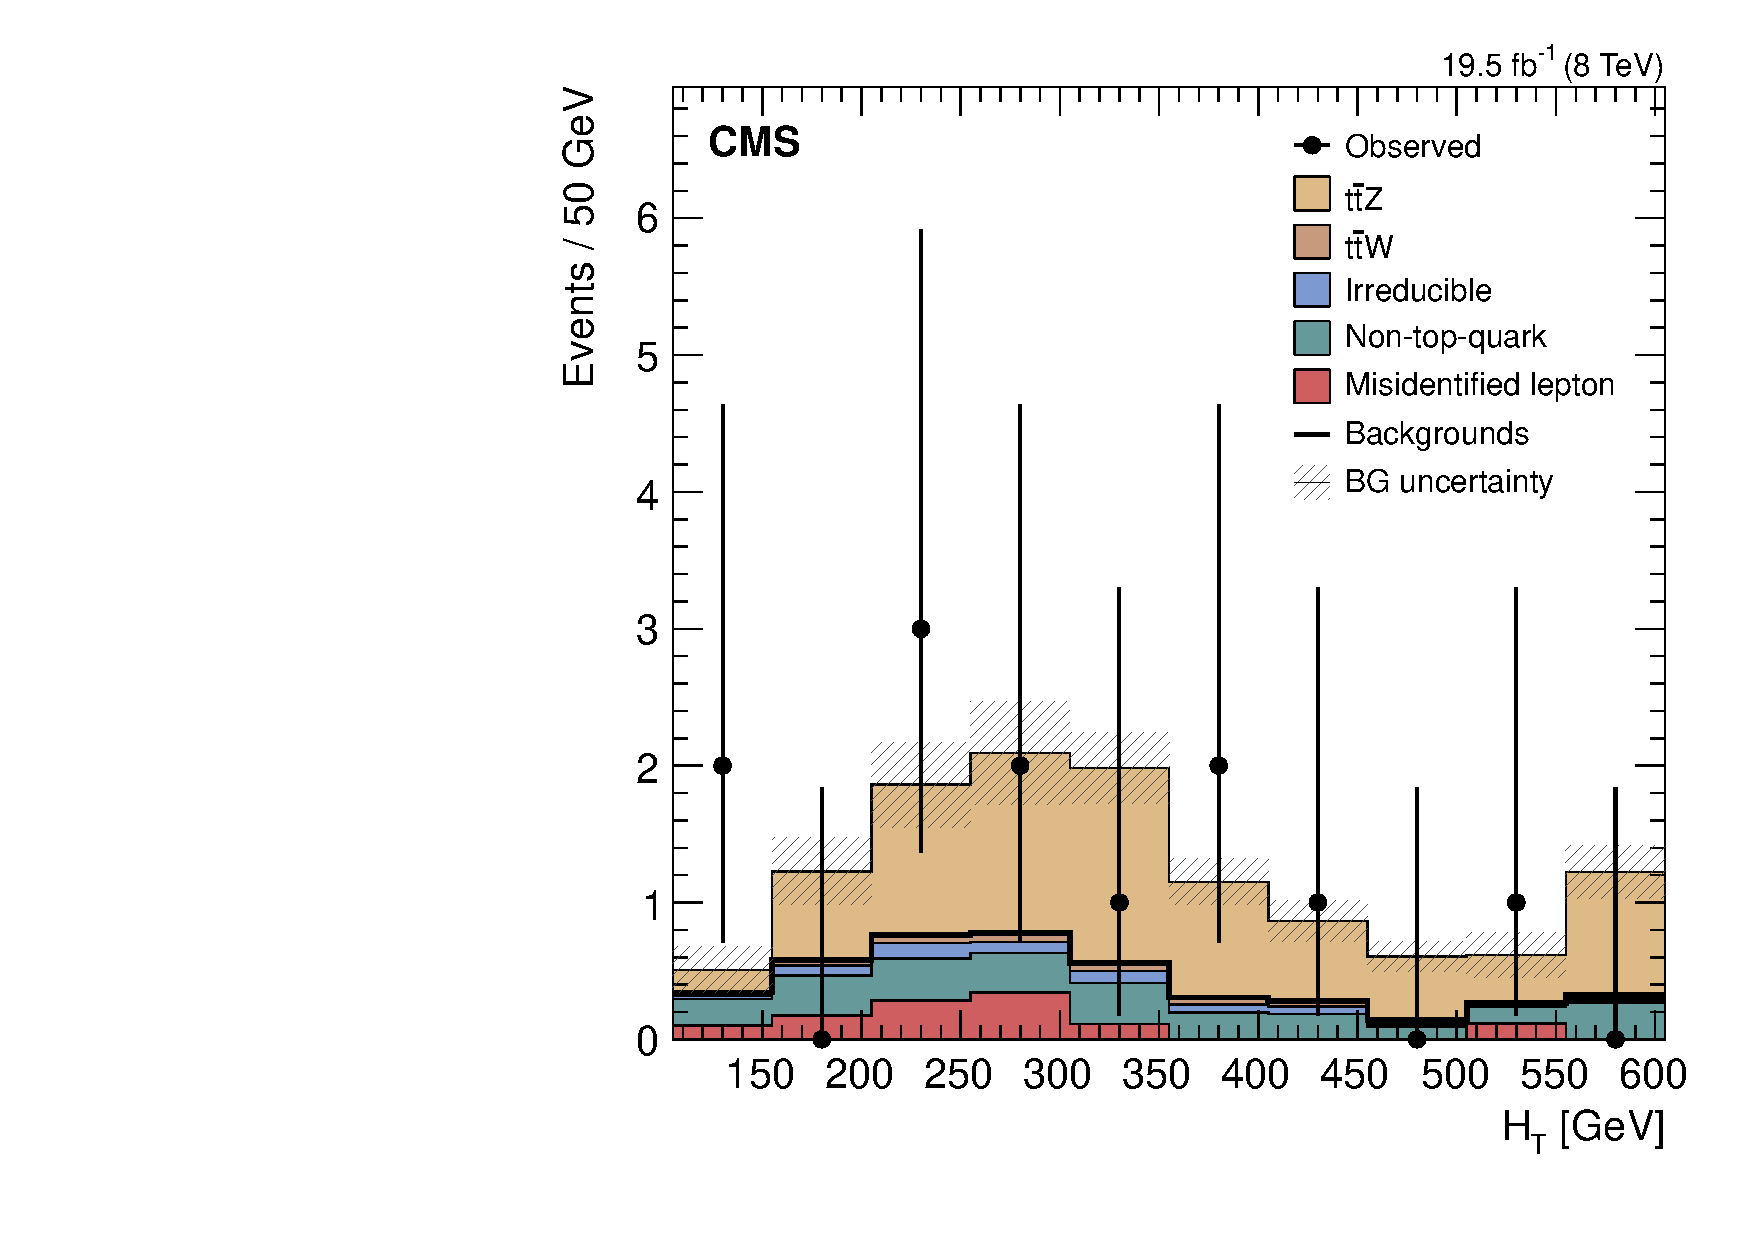
\includegraphics[width=0.7\linewidth]{Figs/Plots_Final_Selections/hHt_3L2J2b.pdf}
\caption{\label{fig:hHt_3l2j2b}
\HT \ of the events after full analysis selections have been applied. This shows general agreement between measured data and predicted signal and backgrounds. 
}
\end{center}
\end{figure} 















	
	
	\section{Cross Section Calculation and Significance}
	The \ttZ \ signal is estimated in Section ~\ref{sec:signal} to be $7.62 \pm 3.46_{data\ st} \pm 0.73_{bkg\ st} \pm 1.37_{bkg\ sy}$. For the luminosity of the full dataset, we use the quoted luminosity of \intLumiwError~\cite{lumi12up}. Finally, we calculate the Branching Ratio (B) multiplied by the Acceptance of selections (A) multiplied by the Efficiency of selections ($\epsilon$) all at once. To do this, we divide the number of \ttZ \ events in MC (using the sample listed in Table ~\ref{tab:IrreducibleMCSamples}) that pass selections by the total number of \ttZ \ events in MC. This gives a BR $\times$ Acc $\times \epsilon$ of $0.0021 \pm 4.0\% _{st} \pm 10.5\% _{sy}$.\\

The full cross section is given by 
%\begin{equation}
%\begin{split}
%        %  \begin{align*}
%         \sigma &= \frac{Yields - Bkg}{\mathcal{L} \times BR \times Acc \times \epsilon}\\
%                      &=  186 \pm 85_{data\ st} \pm 18_{bkg\ st} \pm 33_{bkg\ sy} \pm 7_{BR*Acc*\epsilon\ st} \pm 20_{BR*Acc*\epsilon\ sy} \pm 5_{lumi\ sy}\ fb\\
%                      &= 186 \pm 107\ \text{fb}
%        %  \end{align*}
%        \end{split}
%\end{equation}

\begin{align}
         \sigma &= \frac{Yields - Bkg}{\mathcal{L} \times B \times A\times \epsilon}\\
                      &=  186 \pm 85_{data\ st} \pm 18_{bkg\ st} \pm 33_{bkg\ sy}\pm 7_{B*A*\epsilon\ st} \pm 20_{B*A*\epsilon\ sy} \pm 5_{lumi\ sy}\ \text{fb}\\
                      &= 186 \pm 107\ \text{fb}
\end{align}
          
          
 Additionally, the LandS software is used to perform this calculation with a bit more rigor (see~\cite{higgscomb}). Data cards are prepared from the information contained in this note. Backgrounds are assumed to be log normal with uncorrelated errors. Data driven backgrounds use the statistical and systematic uncertainties that were derived with the methods. Monte Carlo only backgrounds use the uncertainties derived in Sec~\ref{ch:eff_and_unc}. With this preparation, the signal strength (Table~\ref{tab:significance}) and ratio to theory cross section (Table~\ref{tab:landsout}) are found (where again the NLO theory cross section for \ttZ \ production is 205 fb). The final cross section measurement is $\sigma=194 _{-89} ^{+105}$ \ fb and the Ratio to Theory = $0.94 _{-0.43} ^{+0.51}$.\\
 
 
 
\begin{table}[ht!]
\caption{ \label{tab:significance} Expected and measured significance of the signal are shown. Measured significance is in agreement with the expected value.}
\begin{center}
\begin{tabular}{c|c}\hline
	& Significance	 \\ \hline
Expected	& 2.45	 \\
Measured	& 2.33	 \\
\hline
\end{tabular}
\end{center}
\end{table}
 
\begin{table}[ht!]
\caption{ \label{tab:landsout} Measured cross section as calculated by LandS. LandS uses bayesian statistics treating the backgrounds as log normal priors to calculate the cross section.}
\begin{center}
\begin{tabular}{c|cc}\hline
	& r        & Cross Section	 \\ \hline
	&  & \\
\ttZ	& $0.94 _{-0.43} ^{+0.51}$ & 	$194 _{-89} ^{+105}$ fb\\
& & \\
\hline
\end{tabular}
\end{center}
\end{table}
 
 
 
 
 
 
 
 \clearpage
 
 
 \section{Combined Cross Section and Significance}
 The measurement presented in this document relies on measuring the rate of production of the \ttZ process which decays into a try-lepton signature. Other final state signatures could be chosen and different techniques employed to measure the cross section of the \ttZ process in other final decay states. The advantage is that the various final states are statistically independent and thus can be combined for a reduced uncertainty on the measurement. Such a combination was performed using the results in this document as well as those determined in conjunction with Rutgers University and ETH Zurich. The combination is described in~\cite{ttV_combination}. In this combination, the cross section for the production of \ttbar~V is measured as well where V stands for both W and Z bosons. This makes the measurement a generate production of \ttbar in association with vector bosons.\\
 
 The \ttW was measured in several two lepton channels in order to maximize significance from the charge imbalance of the production. \ttZ to four leptons is measured in more than one channel to also maximize the contribution of more significant regions. This produces 9 channels in total.
 
 
 
 To maximize the sensitivity, the nine \ttW and \ttZ channels are combined. A profile likelihood scan is used to evaluate the cross-section central values and corresponding uncertainties. The same statistical procedure used in the discovery of the Higgs boson and combination of the various channels to measure the Higgs was used and 
is described in detail in Ref~\cite{higgscomb}. Table~\ref{tab:combination} summarizes the independent measurements of the various channels.

\begin{table}[!h]
%\tiny
\begin{center}
\caption{\label{tab:combination} Results of the extraction of cross sections, from single and combined channels. 
                                 The significance is expressed in terms of standard deviations.}
\begin{tabular}{c|c|c|c}
\hline
\hline
Channels used & Process &  Cross section & Significance  \\
\hline
2$\ell$ &  \ttW & $170 ^{+90}_{-80} \textrm{(stat.)} ^{+70}_{-70} \textrm{(syst.)}$  fb & 1.6 \\
3$\ell$+4$\ell$ &  \ttZ & $200 ^{+80}_{-70} \textrm{(stat.)} ^{+40}_{-30} \textrm{(syst.)}$ fb & 3.1 \\
2$\ell$+3$\ell$+4$\ell$ & \ttW $+$ \ttZ & $380 ^{+100}_{-90} \textrm{(stat.)} ^{+80}_{-70} \textrm{(syst.)}$ fb & 3.7 \\
%2L+3L+4L & $180 ^{+175}_{-168} \textrm{(total)}$ fb & --- & $218 ^{+159}_{-118} \textrm{(total)}$  fb & --- & --- & --- \\
\hline
\hline
\end{tabular}
\end{center}
\end{table}

\begin{table}[!h]
%\tiny
\begin{center}
\caption{\label{tab:fit2d} Results for the two dimensional fit of the \ttW and \ttZ cross sections. Errors contain both statistical and systematic uncertainties.}
\begin{tabular}{c|c|c}
\hline
\hline
Channels used & \ttW  cross section &  \ttZ{} cross section \\
\hline

2$\ell$+3$\ell$+4$\ell$ & $170 ^{+110}_{-100} \textrm{(total)}$ fb & $200 ^{+90}_{-90} \textrm{(total)}$ fb  \\

\hline
\hline
\end{tabular}
\end{center}
\end{table}



In order to combine the \ttZ channels, a one-dimensional fit is performed on all of the channels. A one-dimensional fit is also performed on the \ttW channels. This fit maximizes the contributions from the most significant channels. From the same-sign dilepton channels, the extracted \ttW cross section is measured to be  $170 ^{+90}_{-80} \textrm{(stat.)} ^{+70}_{-70} \textrm{(syst.)}$~fb, with a significance of $1.6$ standard deviations. The three and four lepton channels combined to a measured \ttZ cross section of 
$200 ^{+80}_{-70} \textrm{(stat.)} ^{+40}_{-30} \textrm{(syst.)}$~fb, with a significance of $3.1$ standard deviations. 

Because each measurement depends on the value of the other process (e.g. \ttZ relies on the \ttW cross section in it's measurement), the cross section of the second process is constrained to the theoretical SM value with a systematic uncertainty of 50\%.

To gauge the impact of using the constrained value, it is varied. The measured \ttW cross section varies by approximately 10\% 
when the theoretical \ttZ cross section is altered up to 1.5 times its nominal theoretical value.  
Performing the same procedure with the \ttW theoretical value, the variation of the measured \ttZ cross section 
is less than 2\%. 

\begin{figure}[!h]
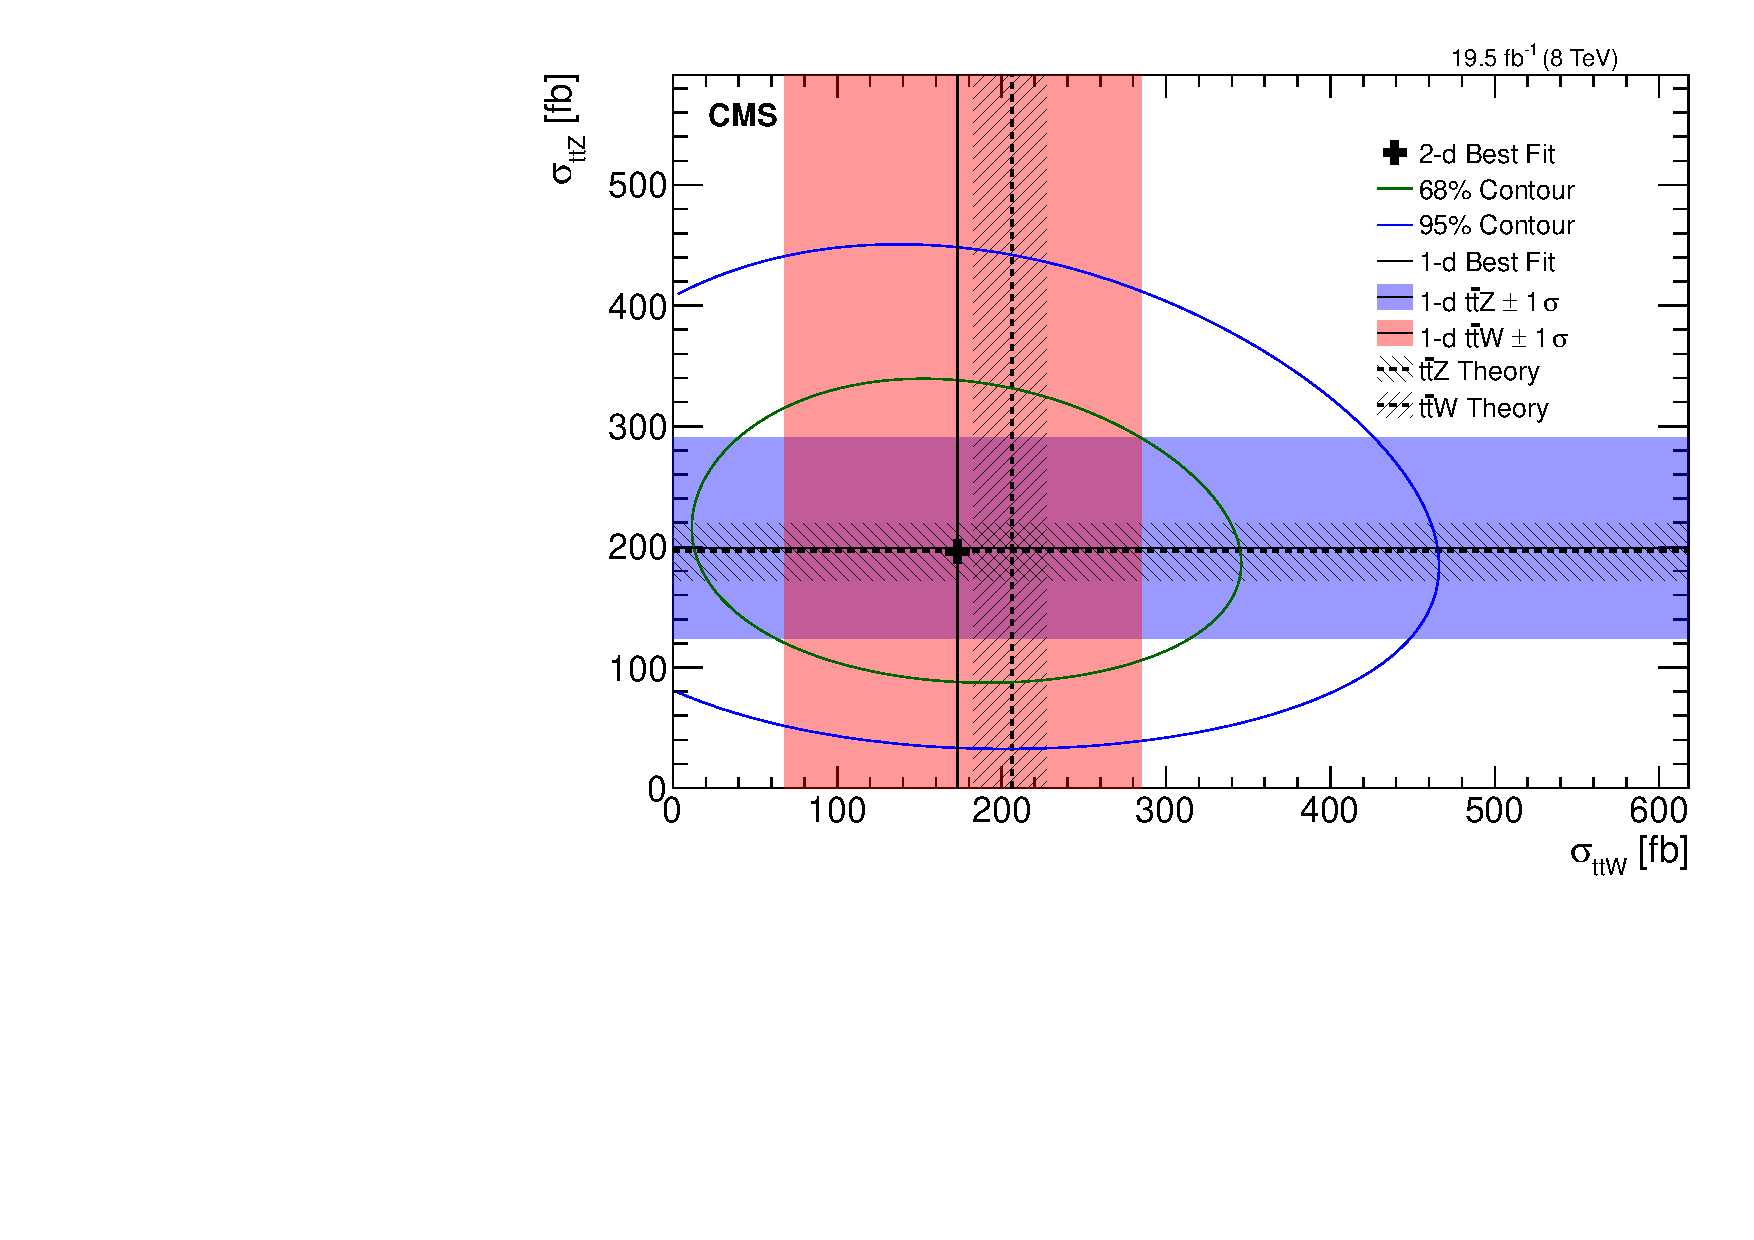
\includegraphics[width=0.97\linewidth]{fit_2d.pdf}
\caption{\label{fig:combination_2d} The result of the two-dimensional best fit for \ttW and \ttZ{} cross sections 
%($\textbf{+}$ symbol) 
(cross symbol) 
is shown along with its 68 and 95\% confidence level contours. The result of this fit is superimposed with the 
separate \ttW and \ttZ{} cross section measurements, and the corresponding 1$\sigma$ bands, obtained 
from the dilepton, and the trilepton/four-lepton channels, respectively. The figure also shows the 
predictions from theory and the corresponding uncertainties.}
\end{figure}

A more sophisticated approach can be taken to allow both measurements to feed back into each other and remove the reliance on the theoretical cross sections. A simultaneous fit is performed on the two processes using all of the channels. The two-dimensional fit is represented graphically in Fig~\ref{fig:combination_2d} and Table~\ref{tab:fit2d} summarizes the cross sections numerically. Within uncertainties the 2 one-dimensional fits and the 1 two-dimensional fit produce the same measurement for the \ttZ and \ttW cross sections.



%
Finally, a one-dimensional fit of all channels is performed to extract a combined cross section 
$\sigma_{\ttbar\textrm{V}} = 380 ^{+100}_{-90} \textrm{(stat.)} ^{+80}_{-70} \textrm{(syst.)}$~fb 
%, where V stands for W or Z, 
with a significance of 3.7 standard deviations. 
%

 
   

% --------------------------------------------------------------------------- %
% --------------------------------------------------------------------------- %
\chapter{Summary and Conclusions}
\label {ch:conclusion}
% --------------------------------------------------------------------------- %
% --------------------------------------------------------------------------- %

This dissertation presents the measurement of the cross section of associated production of top anti-top pairs with Z bosons at $\sqrt{s} = 8 \TeV$. The measurement is an inclusive search performed in a tri-lepton final state. In \intLumi of data, the cross section for \ttZ \ production is measured as $\sigma=194 _{-89} ^{+105}$ \ fb with a significance of 2.33. Finally, the ratio of measured to theoretical cross section is $0.94_{-0.43} ^{+0.51}$.\\

Additionally the results of a combination of this work with the work of other groups has been shown and reports a \ttZ cross section of 
$200 ^{+80}_{-70} \textrm{(stat.)} ^{+40}_{-30} \textrm{(syst.)}$~fb, with a significance of $3.1$ standard deviations. The combined cross section of \ttZ and \ttW (\ttV) is reported as $\sigma_{\ttV} = 380 ^{+100}_{-90} \textrm{(stat.)} ^{+80}_{-70} \textrm{(syst.)}$~fb.\\

\ttZ production will continue to be an important topic as the CMS Experiment looks towards future runs of the LHC at 13 and 14 \TeV center-of-mass energy collisions. The work done here helps to experimentally constrain and measure the \ttZ production cross section which, aside from the indepentent achievement of measuring a SM phenomenon, will help to guide MC simulations used for estimating backgrounds and desiging background subtraction techniques for New Physics searches. \ttZ searches at higher energy and with more integrated luminosity measured in the future, will prove invaluable to help measure the weak coupling interactions of the top quark as one of the main diagrams contributing to \ttZ production involves direct coupling of the Z boson to the top quark.\\ 


\bibliographystyle{lucas.bst}
\bibliography{include/refs}

\appendix


\end{document}
